\documentclass[12pt,a4paper,openany,final,twoside,longbibliography,hidelinks]{book}
\usepackage{acronym}
\usepackage[english]{babel}
\usepackage[utf8]{inputenc}
\usepackage[T1]{fontenc}
\usepackage{amsmath}
\usepackage{mathtools}
\usepackage{amsfonts}
\usepackage{amssymb}
\usepackage{bbold}
\usepackage{esdiff}
\usepackage[]{graphicx}
\usepackage[sort&compress,numbers]{natbib}
\bibliographystyle{unsrtnat}
% \bibliographystyle{aipnum4-2}
\usepackage{doi}
\renewcommand*{\bibfont}{\interlinepenalty 10000\relax}
\usepackage[defaultlines=2,all]{nowidow}
\usepackage{siunitx}
\sisetup{range-phrase=--}
\sisetup{range-units=single}
 
\usepackage[dvipsnames]{xcolor}
\usepackage{bm}
\usepackage{float}
\usepackage{verbatim}
\usepackage{afterpage}
\usepackage{microtype}
\usepackage[labelfont=bf]{caption}
\captionsetup[table]{position=above}
\usepackage{subfigure} 
\usepackage[onehalfspacing]{setspace}
\usepackage{blindtext} 
\numberwithin{equation}{section}
\usepackage{etoolbox}
\graphicspath{{./images/}}
\usepackage[]{geometry}
\usepackage[nottoc,notlof]{tocbibind}
\usepackage[ddmmyyyy]{datetime}
\renewcommand{\dateseparator}{.}
\usepackage{feynmf}
\usepackage{fancyhdr} 

\pagestyle{fancy}
\renewcommand{\chaptermark}[1]{\markboth{\thechapter.\space#1}{}} 

\fancypagestyle{schluss}{
    \fancyhead{}
    \fancyfoot[EL]{\thepage} 
    \fancyfoot[OR]{\thepage}
    \renewcommand{\headrulewidth}{0pt}}\graphicspath{{./images/}}
    
\fancyhf{}  % Kopf- und Fußzeile leeren 
\makeatletter
\let\ps@plain\ps@fancy
\makeatother

\fancypagestyle{myfancy}{
\newcommand{\lmod}{\fontfamily{lmodern}\fontsize{9}{11}\selectfont}
\fancyhead[EL,OL]{\lmod \nouppercase{\scshape\leftmark}} 
\fancyhead[ER,OR]{\lmod \nouppercase{\scshape\rightmark}} 
\fancyfoot[EL]{\lmod\thepage} 
\fancyfoot[OR]{\lmod\thepage}} 
\renewcommand{\chaptermark}[1]{\markboth{\thechapter.\space#1}{}} 


\fancypagestyle{schluss}{
    \fancyhead{}
    \fancyfoot[EL]{\thepage} 
    \fancyfoot[OR]{\thepage}
    \renewcommand{\headrulewidth}{0pt}}
\fancyhf{} 




\newcommand{\sg}[1]{\textcolor{blue}{#1}}
\newcommand{\ui}[1]{\textcolor{Green}{#1}}

\DeclareMathOperator{\Tr}{Tr}
\newcommand{\red}[1]{\textcolor{red}{#1}}
\newcommand{\wert}[3]{\SI[separate-uncertainty=true]{#1(#2)}{#3}}
\newcommand{\abs}[1]{\ensuremath{\left\vert#1\right\vert}}
\newcommand{\ket}[1]{\ensuremath{\left\vert #1\right>}}
\newcommand{\bra}[1]{\ensuremath{\left<#1\right\vert}}
\newcommand{\kasten}[1]{\mbox{\color{#1}$\blacksquare$}}
\newcommand{\rgbbox}[1]{\mbox{\color[RGB]{#1}$\blacksquare$}}
\newcommand{\hexbox}[1]{\mbox{\color[HTML]{#1}$\blacksquare$}}
\newcommand{\dint}[1]{\ensuremath{\mathop{\mathrm{d}#1}}}
\newcommand{\vect}[1]{\mathbf{#1}}


\usepackage{lmodern}
\makeatletter
\patchcmd{\BR@backref}{\newblock}{\newblock(\mbox{on thesis page}~}{}{}
\patchcmd{\BR@backref}{\par}{)\par}{}{}
\makeatother




\begin{document}

\pagenumbering{gobble}

\begin{titlepage}
    \begin{center}
	{\scshape\Large Dissertation\\}
	\vspace{.1cm}
	\rule[1pt]{\textwidth}{1.5pt}
    \LARGE{\textbf{Automated optimization of sensitivity in a search for boosted VBF Higgs pair production in the $b\overline{b}b\overline{b}$ quark final state with the ATLAS detector
	}}
    \rule[11pt]{\textwidth}{1.5pt}
	
    {\normalsize\textbf{For the attainment of the academic degree doctor rerum naturalium (Dr. rer. nat.) in the subject: Physics}} 
    \vspace{1cm}

    \Large{\textbf{M.Sc. Frederic Renner\\}}
	Berlin, \today\\
    \vspace{1cm}
    \large
	Faculty of Mathematics and Natural Sciences of the Humboldt University of Berlin\\
    \vspace{1cm}

	1st Supervisor: Dr. Clara Elisabeth Leitgeb\\
	2nd Supervisor: Prof. Dr. Cigdem Issever
	\vspace{01cm}


	\newpage 
	(Only after the disputation for publication in the university library according to § 15	of the doctoral regulations enter the names and the date):\\
	\raggedright
	Reviewers: \\
	1st: \\
	2nd: \\
	3rd: \\
	
	Date of the oral examination: 
\end{center}
\end{titlepage}

\newpage 
\quad
\thispagestyle{empty}

\newpage 
\thispagestyle{empty}
\begin{center}
    \textbf{Abstract}
\end{center}
%\vspace{.5cm}
\noindent I am an abstract.

\newpage
\quad
\thispagestyle{empty}

\setcounter{tocdepth}{1}
\tableofcontents

% \newpage
% \thispagestyle{empty}
% \listoffigures


\newpage
\quad
% \thispagestyle{empty}



\newpage 
\thispagestyle{empty}
\quad  

\newpage
\thispagestyle{empty}
\pagestyle{myfancy}
\pagenumbering{arabic}


%-------------------------------------------------------------


% \chapter{Introduction}


https://arxiv.org/pdf/2207.00043.pdf

mehr gründe warum physik versteckt in top und higgs präziosions messungen... 
% \part{Overview}
\chapter{The Standard Model of Particle Physics}\label{ch:sm}
\noindent The \ac{sm} of Particle Physics is the current theory that describes three of the four fundamental forces, namely the electromagnetic, strong, and weak forces, with the exception of gravity. Over the last decades it has been probed with remarkable precision. However, as discussed later in this chapter, there are still observational phenomena that lie beyond its scope.

The \ac{sm} is described by a lorentz-invariant \ac{qft} that is renormalizable and invariant under local gauge transformations. This means that within the non-abelian gauge group
\begin{equation}
    G = SU(3)_C \otimes SU(2)_L \otimes U(1)_Y,
\end{equation}
the equations of motions remain invariant. $SU(3)_C$ is the special unitary group of rank 3 representing the color symmetry within \ac{qcd}, the \ac{qft} describing the strong interactions. $SU(2)_L \otimes U(1)_Y$ exhibits the unification of the weak and electromagnetic interaction into the \ac{ew} force with symmetries for $SU(2)_L$ left-chiral particle doublets and the unitary group $U(1)_Y$ for particles carrying weak hypercharge $Y$.

The following describes the particles of the \ac{sm} and gives a brief overview of the \ac{qft}'s used to describe aforementioned forces. The content of this chapter draws inspiration primarily from \citep{hollik2010quantum,griffiths2020introduction,thomson2013modern,zee2010quantum,halzen1984introductory}. Natural units are assumed everywhere $(\hbar=c=1)$.


\section{Particles of the Standard Model}

All currently known elementary particles are included in the \ac{sm} and can be organized as depicted in figure \ref{fig:sm}. This includes 12 fermions, that are particles of half-integer spin, 12 vector bosons with spin 1, and the Higgs boson, a scalar particle with spin 0.


\begin{figure}
    \centering
    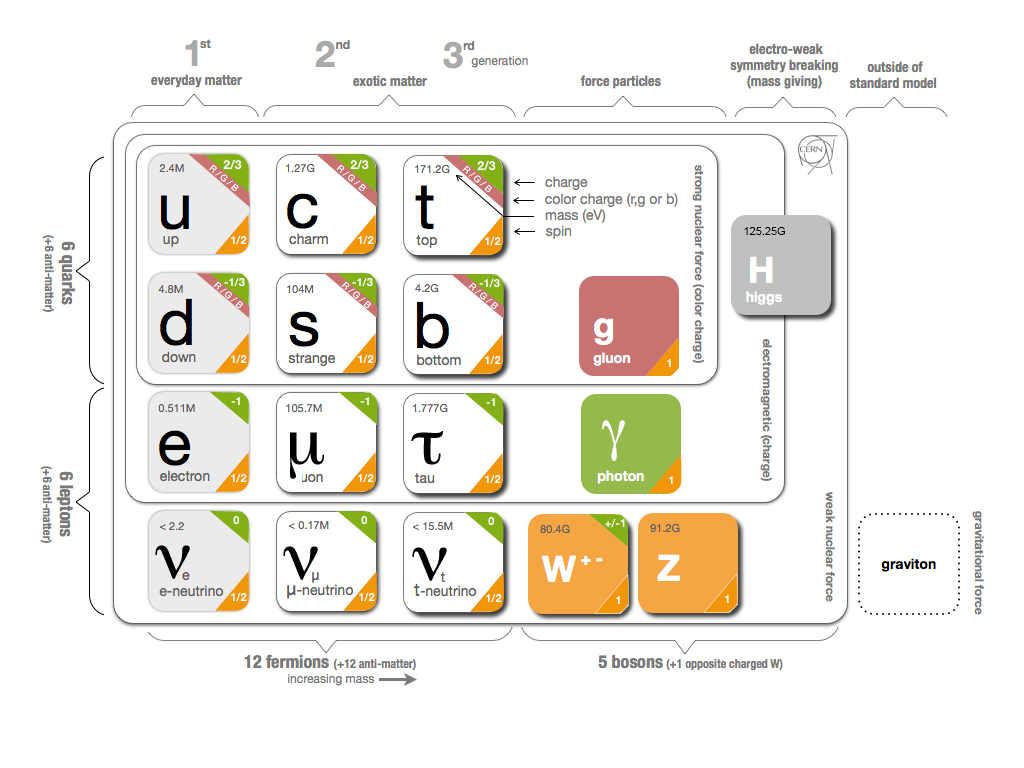
\includegraphics[width=1\textwidth]{SMinfographic_image_}
    \caption[]{Particles in the SM. Adopted from \citep{smpar}. The Higgs Boson mass is corrected to the current value \citep{particle2022review}. }
    \label{fig:sm}
\end{figure}


The fermions can be categorized into three generations each consisting of a charged lepton, a neutral neutrino and two quarks. Except for their masses, particles of different generations have the same quantum numbers. Ordinary matter consists only of particles from the first generation. Moreover each particle has an associated anti-particle with all the quantum numbers inversed.

Quarks possess both electroweak and color charges, causing them to interact with each other via weak, electromagnetic, and strong forces. Each generation consists of an up-type quark (up, charm and top quark) with an electric charge in units of the electron charge of \mbox{Q = + 2/3$e$} and a down-type quark (down, strange and bottom quark) with \mbox{Q = -1/3$e$}. Due to color confinement, quarks can only be observed as composite particles called hadrons, a principle of \ac{qcd} discussed in section \ref{sec:qcd}. Prominent hadrons include mesons (two quarks, e.g., pion) and baryons (three quarks, e.g., proton).

Leptons, which do not carry a color charge, include the electron $e$, muon $\mu$, tau $\tau$, and their associated neutrinos $\nu_e$, $\nu_\mu$, and $\nu_\tau$. Neutrinos have very small masses compared to other particles and are considered massless within the theoretical framework of the \ac{sm}. Neutrinos do not carry an electric charge and interact solely via the weak force, while charged leptons ($e$, $\mu$, $\tau$) with charge $Q=-1$ also interact electromagnetically.

Fermions interact with fields via bosons specific to each force. The strong force is mediated by eight massless gluons $g$, while the electroweak theory includes four massless bosons $W_1,W_2,W_3,B$.

The scalar Higgs particle plays a unique role in the \ac{sm}, breaking the electroweak interaction into weak and electromagnetic interactions through the Higgs mechanism. This process, detailed in section \ref{sec:higgs_mechanism}, explains the observed masses of weak interaction mediators $W^{\pm}$ and $Z$ and also provides an interpretation of the origins of mass for fermions.

If not specified otherwise the following discussions always includes the anti-particles when referred to a species or a particular particle.

\section{Elements of Quantum Field Theory}\label{sec:qft}
Elementary particles can be created, transformed, and annihilated in various forms of particle interactions. These phenomena can be understood through special relativity and quantum mechanics. Special relativity relates energy with mass, allowing energy to manifest as massive particles and vice versa. Quantum mechanics, through the uncertainty principle, states that energy can fluctuate significantly over short time scales.

However, special relativity lacks a quantum mechanical description, and in non-relativistic quantum mechanics, the particle number is conserved. \ac{qft} was developed to provide a solution to this dilemma and to incorporate observations from both fields into a unified theory.

For a field description, some quantity $\phi(x,y,z,t)=\phi(x)$ is assigned to some region in spacetime $x$. Similar to the Lagrangian formalism in classical mechanics, here a Lagrangian density in spacetime governs the dynamics of the system $\mathcal{L}(\phi_1,\dots,\phi_n) =T-V$. Fields which appear in the \ac{sm} and their associated Lagrangians are summarized in table \ref{tab:fields}.
{\renewcommand{\arraystretch}{1.7} %<- modify value to suit your needs
\begin{table}
    \begin{center}
        \begin{tabular}{c|c|c}
            particle           & field type      & Lagrangian                                                                                                   \\ \hline
            spin-0 (scalar)    & scalar $\phi$   & $\mathcal{L}_\mathrm{Klein-Gordon}=\frac{1}{2} (\partial_\mu \phi )(\partial^\mu \phi)-\frac{m^2}{2}\phi^2 $ \\
            spin-1/2 (fermion) & spinor $\psi$   & $\mathcal{L}_\mathrm{Dirac}= \overline{\psi}(i \gamma^\mu \partial_\mu - m )\psi$                            \\
            spin-1 (boson)     & vector  $A_\mu$ & $\mathcal{L}_\mathrm{Proca}= -\frac{1}{4}F_{\mu\nu}F^{\mu\nu} +\frac{m^2}{2} A_\mu A^\mu$                    \\ [.7ex]
        \end{tabular}
        \caption{Quantum fields relevant for the \ac{sm}. With $F_{\mu\nu}=\partial_\mu A_\nu - \partial_\nu A_\mu$ the electromagnetic field strength tensor.}
        \label{tab:fields}
    \end{center}
\end{table}
}
% Via the generalized Euler-Lagrange equations of \ac{qft} 
% \begin{equation}
%     \partial_\mu \left(\frac{\partial\mathcal{L}}{\partial(\partial_\mu\phi_i)}\right)=\frac{\partial\mathcal{L}}{\partial \phi_i}.
% \end{equation}
% the according equations of motion associated with the fields can be obtained.

In \ac{qft} the conventional strategy to describe particle dynamics is to use a perturbation ansatz $\mathcal{L}=\mathcal{L}_0+\mathcal{L}_1$ where one knows the solution of $\mathcal{L}_0$ and adds a small perturbation $\mathcal{L}_1$ so that $\mathcal{L}$ can be solved \citep{zee2010quantum}. Here the free field/kinetic part of the Lagrangian is \mbox{$\mathcal{L}_0=\frac{1}{2}[(\partial_\mu \phi)^2 - m^2\phi^2] $} and a small perturbation/potential term $\mathcal{L}_1=V(\phi)$ is added as some polyominal in $\phi$ that governs the interactions of particles. A term $J(x)\phi(x)$ needs to be added to excite the field or create/destroy particles so that the ansatz reads
\begin{equation}
    \mathcal{L}=\frac{1}{2}[(\partial_\mu \phi)^2 - m^2\phi^2]
    -V(\phi) + J(x)\phi(x).
\end{equation}
In the path integral formulation of \ac{qft} the problem can be reduced to integrals of the form \mbox{$\int D\phi e^{i\int d^4x \mathcal{L}(\phi(\bm{x},t))}$}. Where $\int D\phi$ is the integral over all possible paths of the field. Usually the perturbation $V(\phi)$ is just one anharmonic term with $\lambda\phi^4$ with coupling strength $\lambda$ and is expanded in $e$ to make the integral solvable
\begin{equation}
    e^{-V(\phi)}=e^{-\lambda\phi^4}=1-\lambda\phi^4+\frac{1}{2}\lambda^2\phi^8+\dots
\end{equation}
This only works if $\lambda$ is small. With this the Lagrangian can be solved and the result is a probability also called the amplitude usually denoted with $\mathcal{M}$. Via this one can derive the Feynman rules and calculate cross-sections to a desired order of expansion.

The forces and Lagrangians occurring in the \ac{sm} are discussed in the following sections on \ac{qed} \ref{sec:qed}, \ac{qcd} \ref{sec:qcd} and the \ac{ew} theory \ref{sec:ew}. For these the principle of local gauge invariance plays a key role and is inspired by gauge invariance from classical electrodynamics.

\section{Quantum Electrodynamics}\label{sec:qed}
The \ac{qft}-description of the electromagnetic interaction \ac{qed} can be derived from the free fermion field given by the Dirac equation
\begin{equation}
    \mathcal{L}_\mathrm{Dirac} = \overline{\psi}(i \gamma^\mu \partial_\mu - m )\psi.
    \label{eq:dirac}
\end{equation}
This Lagrangian is invariant, i.e. the equations of motion remain unchanged, under a change of a global phase $\alpha$
\begin{equation}
    \psi(x) \rightarrow  e^{-i \alpha}\psi(x).
\end{equation}
The requirement that this transformation also holds locally means that $\alpha$ now additionally depends on the point $x$ in spacetime $\alpha \rightarrow \alpha(x)$. Since this gives another term because of the derivative, the Lagrangian can be made invariant again by introducing a vector field $A_\mu$ with a coupling of the size of the electron charge $e$ and replacing the derivative $\partial_\mu$ by the covariant derivative $D_\mu$
\begin{equation}
    \partial_\mu \rightarrow D_\mu = \partial_\mu + ie A_\mu.
    \label{eq:cov_diff}
\end{equation}
Thus, the new Lagrangian
\begin{equation}
    \mathcal{L} = \overline{\psi}(i \gamma^\mu D_\mu - m )\psi
    =
    \underbrace{\overline{\psi}(i \gamma^\mu \partial_\mu - m )\psi}_{\mathcal{L}_\mathrm{Dirac} }
    +
    \underbrace{ e\overline{\psi} \gamma^\mu {\psi}A_\mu}_{\mathcal{L}_\mathrm{int}}
\end{equation}
becomes invariant under the local gauge transformations
\begin{align}
    \psi(x)  & \rightarrow  e^{-i \alpha(x)}\psi(x),                      \\
    A_\mu(x) & \xrightarrow{} A_\mu(x) -\frac{1}{e}\partial_\mu\alpha(x),
\end{align}
forming the electromagnetic $U(1)_{EM}$ gauge group.
% The particular scheme of these replacements is also called the minimal substitution rule. 
This Lagrangian describes two fermions interacting with a vector field $A_\mu$ - the photon - represented by the fundamental interaction vertex of \ac{qed} in figure \ref{fig:qed_fundamental}.
\begin{figure}
    \centering
    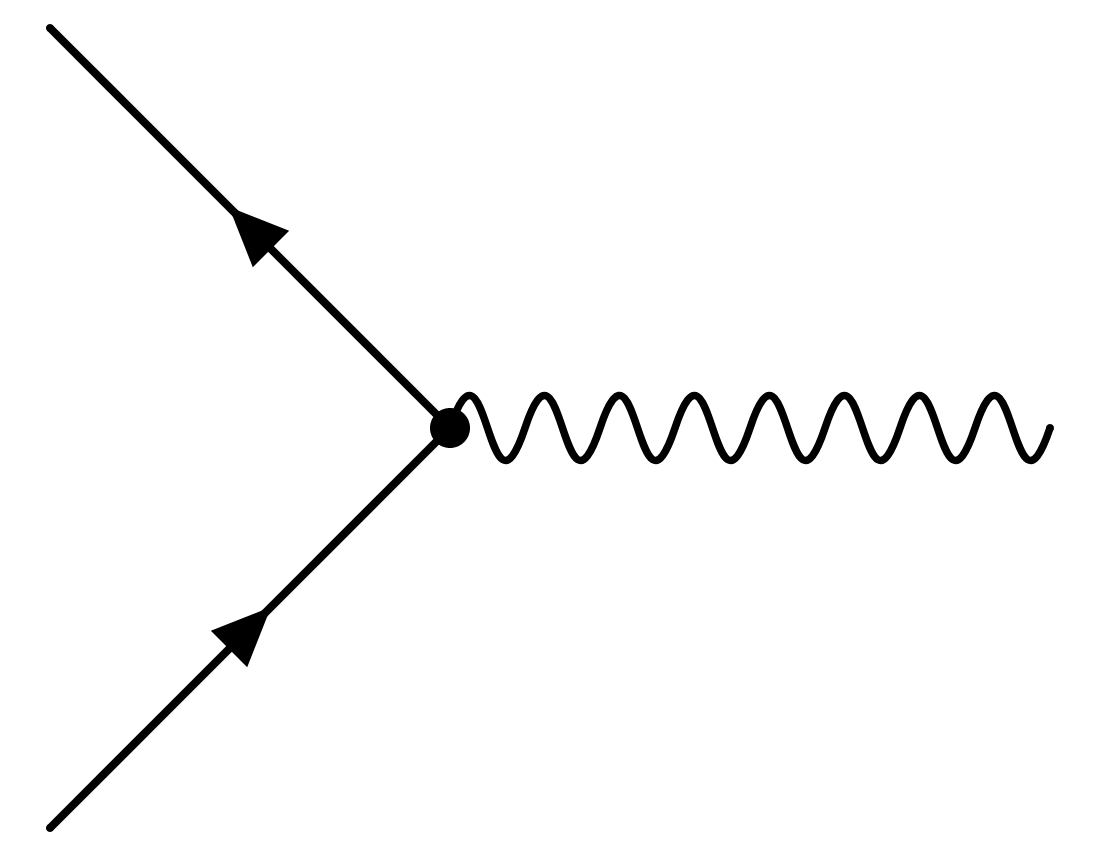
\includegraphics[width=0.27\textwidth]{qed_fundamental}
    \caption[]{The Fundamental interaction vertex of \ac{qed}. Two fermions interacting with a massless photon.}
    \label{fig:qed_fundamental}
\end{figure}
The dyanmics for the photon can be added with the spin-1 Proca Lagrangian from table \ref{tab:fields}. The $F_{\mu\nu}$ term is local gauge invariant whereas $A_\mu A^\mu$ is not, since it picks up a second derivative for $\alpha$ and therefore is required to be massless. The full \ac{qed} lagrangian then reads
\begin{equation}
    \mathcal{L}_\mathrm{QED}
    =
    \underbrace{\overline{\psi}(i \gamma^\mu \partial_\mu - m )\psi}_{\mathcal{L}_\mathrm{Dirac} }
    +
    \underbrace{ e\overline{\psi} \gamma^\mu {\psi}A_\mu}_{\mathcal{L}_\mathrm{int}}
    -
    \underbrace{\frac{1}{4}F_{\mu\nu}F^{\mu\nu}}_{\mathcal{L}_\mathrm{Maxwell} }.
    \label{eq:l_qed}
\end{equation}
That this symmetry holds locally for all unitary $1\times1$ matrices $U(1)$ might seem extravagant, but the formalism is extendable to higher orders as for the \ac{ew} theory and \ac{qcd} case. The gauge group is abelian as any $1\times1$ matrix also commutes with itself. As a result there are no self-interaction terms like $A_\mu A^\mu$ for photons. This means photons only interact with charged particles and not with each other.

\section{Quantum Chromodynamics}\label{sec:qcd}

In a manner similar to how \ac{qed} is derived in section \ref{sec:qed}, the theory of strong interactions, known as \ac{qcd}, is formulated as a non-abelian gauge theory based on the symmetry group $SU(3)$. This group is characterized by the $3\times 3$ Gell-Mann matrices $\lambda_a$ where $a\in\{1,\ldots,8\}$. The fundamental charge in this theory is color, and each quark is represented as a triplet of the three color fermion fields $\Psi_k=(\psi_r,\psi_g,\psi_b)^T$ for all quark flavors $k$. Local gauge invariance of the Lagrangian
\begin{equation}
    \mathcal{L} =
    \sum_k
    \begin{pmatrix}
        \overline{\psi}_r & \overline{\psi}_g & \overline{\psi}_b
    \end{pmatrix}
    (i \gamma^\mu \partial_\mu - m_k )
    \begin{pmatrix}
        \psi_r \\
        \psi_g \\
        \psi_b
    \end{pmatrix}
    =
    \sum_k
    \overline{\Psi}_k(i \gamma^\mu \partial_\mu - m_k )\Psi_k,
    \label{eq:dirac}
\end{equation}
requires the spinors to be invariant under the transformation
\begin{equation}
    \Psi_k(x) \rightarrow e^{i \alpha_a(x) \lambda_a/2} \Psi_k(x),\qquad \alpha\in\mathbb{R},\quad a\in\{1,\mathellipsis,8\},
\end{equation}
with $\alpha_a(x)$ a local phase and the index $a$ for the 8 gluons. It is noted here that summation over equal indices $\alpha_a(x) \lambda_a=\sum_a \alpha_a(x) \lambda_a$ is assumed. As in \ac{qed} a covariant derivative is introduced
\begin{equation}
    D_\mu = \partial_\mu - i g_s \frac{\lambda_a}{2}G_\mu^a,
\end{equation}
involving the eight gluon vector fields $G_\mu^a$ and the coupling strength $g_s$, which is related to the strong coupling constant as
\begin{equation}
    \alpha_s=\frac{g_s^2}{4\pi}.
\end{equation}
With the gluon field strength tensor
\begin{equation}
    G^a_{\mu\nu}=\partial_\mu G_\nu^a-\partial_\nu G_\mu^a+g_s f^a_{\beta\gamma}G^\beta_\mu G_\nu^\gamma, \qquad \text{with } [\lambda_a,\lambda_b]= i f_{ab}^c \lambda_c,
\end{equation}
the gauge invariant \ac{qcd} Lagrangian is
\begin{align}
    {\mathcal {L}}_{\text{QCD}} & =\sum_k\overline{\Psi}_k\left( i \gamma^\mu D_\mu-m_k\right)\Psi_k-{\frac {1}{4}}G_{\mu \nu }^{a}G^{a\mu \nu} \\
                                & =\sum_k
    \underbrace{{\overline{\Psi}_k}\left(i\gamma^\mu \partial_\mu-m_k\right)\Psi_k}_{\mathcal{L}_\text{Kin}}
    \;+ \;
    \underbrace{g_s{\overline{\Psi}_k}\gamma ^{\mu }\frac{ \lambda_a}{2} \Psi_k G_\mu^a}_{\mathcal{L}_\text{Int}}
    \;-\;
    \underbrace{\frac{1}{4}G_{\mu \nu }^{a}G^{a\mu \nu}}_{\mathcal{L}_\text{Self}} .
    \label{eq:l_qcd}
\end{align}
This Lagrangian consists of a kinetic term for each quark, an interaction term of the quarks with the gluons and gluon-gluon interactions resulting in vertices shown in figure \ref{fig:qcd_vertices}. These interactions become apparent when $G^a_{\mu\nu}$ is squared, leading to cubic and quartic terms for the fields.

\begin{figure}[H]
    \centering
    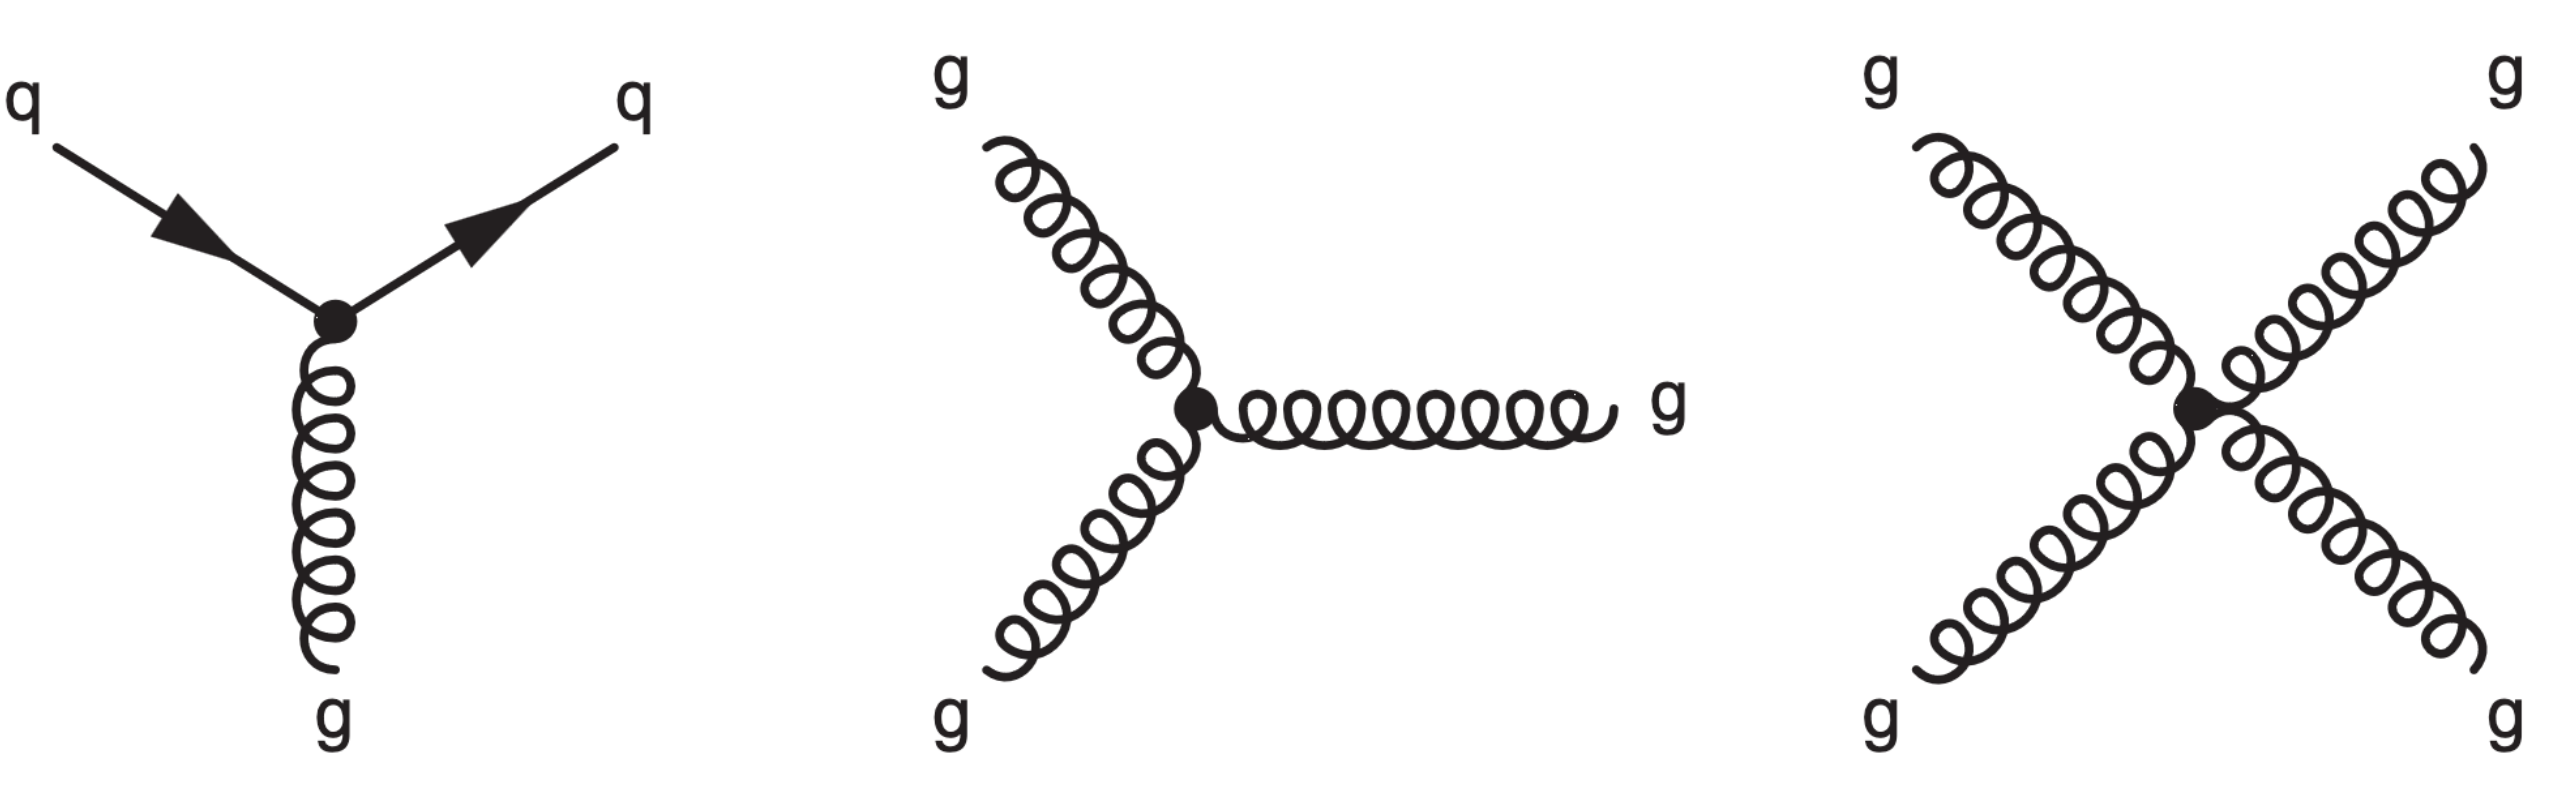
\includegraphics[width=0.8\textwidth]{gluon_gluon_interactions}
    \caption[]{(left) Quarks interacting with a gluon. (middle) triplet and (right) quartic self coupling of gluons. Adopted from \citep{thomson2013modern}.}
    \label{fig:qcd_vertices}
\end{figure}

A unique aspect of \ac{qcd} is color confinement, which states that quarks cannot be observed as free particles; they are always confined within hadrons. This principle arises from the nature of the strong force, which becomes stronger as quarks are pulled apart, a concept further discussed in \ref{sec:renormalization}. Attempts to dissociate hadrons into their quark constituents fails because the formation of quark-antiquark pairs is energetically favoured over separation. This leads to the creation of new hadrons instead of isolated quarks, ensuring that observable particles are always color-neutral.


\section{Electroweak Unification}\label{sec:ew}
The weak force can be incorporated into a gauge-invariant formalism by using a $SU(2)$ symmetry. This is further combined with the electromagnetic force to derive a unified framework for both forces, known as the electroweak interaction, which is described by the symmetry group $SU(2)_L \otimes U(1)_Y$. In this framework, the weak force interacts exclusively with left-handed chiral states of particles, such as for a left-handed fermion $\psi_L$ as expanded on below. Fermions can be grouped by their characteristics into left handed doublets
\begin{equation}
    \begin{pmatrix}
        \nu_e \\ e
    \end{pmatrix}_L, \;
    \begin{pmatrix}
        \nu_\mu \\ \mu
    \end{pmatrix}_L, \;
    \begin{pmatrix}
        \nu_\tau \\ \tau
    \end{pmatrix}_L, \;
    \begin{pmatrix}
        u \\ d
    \end{pmatrix}_L, \;
    \begin{pmatrix}
        c \\ s
    \end{pmatrix}_L, \;
    \begin{pmatrix}
        t \\ b
    \end{pmatrix}_L, \;
    \label{eq:weak_doublets}
\end{equation}
with weak isospin $I=1/2$ that has as third component $I_3=\pm1/2$ for the upper and lower doublet particle respectively. In contrast right handed singlets have $I=0$
\begin{equation}
    e_R    ,\quad \mu_R ,\quad    \tau_R ,\quad    u_R,\quad d_R ,\quad    c_R ,\quad s_R ,\quad    t_R ,\quad b_R.
    \label{eq:weak_singlets}
\end{equation}
The relation between the electric charge of the particle $Q$, $I_3$ and its weak hypercharge $Y$ is governed by the Gell-Mann-Nishijima formula
\begin{equation}
    Q=I_3+Y/2.
    \label{eq:gellmann_nishijima_formula}
\end{equation}
The electroweak Lagrangian is then composed of four basic terms
\begin{equation}
    \mathcal{L}_\mathrm{EW} = \mathcal{L}_\mathrm{fermions}+\mathcal{L}_\mathrm{gauge}+\mathcal{L}_\mathrm{Higgs}+\mathcal{L}_\mathrm{Yukawa}.
    \label{eq:L_EW}
\end{equation}
Following the same steps as for \ac{qcd} and \ac{qed} the Lagrangian can be rendered gauge invariant by introducing a covariant derivative and gauge fields that are dictated by the group symmetry.

$SU(2)$ is generated through the three Pauli matrices $\bm{\sigma}$ requiring three vector gauge fields $W^a_\mu$, $a=\{1,2,3\}$ whereas the $U(1)$ symmetry of the vector gauge field $B_\mu$ is generated by the weak hypercharge $Y$ so the Lagrangian needs to be invariant under the transformation
\begin{align}
    \psi_{L} & \rightarrow e^{i \alpha_a(x) \sigma_a/2}e^{ iY/2} \psi_{L},\qquad & a\in\{1,\mathellipsis,3\} ,\quad \alpha\in\mathbb{R} & \label{eq:gauge_transformation_left}
    \\
    \psi_{R} & \rightarrow e^{ i\beta(x) Y/2} \psi_{R},\qquad                    & \beta\in\mathbb{R}                                   & \label{eq:gauge_transformation_right}
\end{align}
% At this stage the new vector fields are still massless and give the fermionic and gauge parts of the Lagrangian and will be explained below. The masses for the fermions and bosons can be incorporated via the Higgs mechanism that is described in section \ref{sec:higgs_mechanism} yielding the Higgs and Yukawa parts of the Lagrangian.


\subsubsection*{Fermion term}
To distinguish left-handed and right-handed particle states, the corresponding spinors can be written as
\begin{equation}
    \psi_L=\frac{1-\gamma^5}{2}\psi, \quad \psi_R=\frac{1+\gamma^5}{2}\psi,
\end{equation}
where the fifth gamma matrix is defined in terms of the other four gamma matrices as $\gamma^5 = i \gamma^0 \gamma^1 \gamma^2 \gamma^3$. The concept of helicity, which is the projection of a particle's spin along its momentum direction, is useful in understanding these states. However, $\psi_{L}$ and $\psi_{R}$ are not helicity eigenstates but rather select the spinor $\psi$ with the corresponding helicity and vanishes otherwise:
\begin{equation}
    \frac{1}{2}(1 \pm \gamma^5)\psi =
    \begin{cases}
        0    & \text{if } \psi \text{ has helicity } \mp1, \\
        \psi & \text{if } \psi \text{ has helicity } \pm1.
    \end{cases}\label{eq:left_handed_state}
\end{equation}
The aforementioned doublets and singlets are then represented by
\begin{equation}
    \psi_L^j=
    \begin{pmatrix}
        \psi_{L+}^j \\ \psi_{L-}^j
    \end{pmatrix},
    \quad \psi_{R\xi}^k,
\end{equation}
with $j$ running over the doublets from equation \ref{eq:weak_doublets}, $k$ over the singlets from equation \ref{eq:weak_singlets} and $\xi=+$ for u-type fermions and $\xi=-$ for d-type fermions.
The covariant derivative is
\begin{align}
    D_\mu^L & =\partial_\mu- i g_2 \frac{{\sigma}_a}{2}W_\mu^a+i g_1\frac{Y}{2}B_\mu, \label{eq:cov_diff_L} \\
    D_\mu^R & =\partial_\mu+ i g_1\frac{Y}{2}B_\mu,
\end{align}
with coupling $g_2$ and $g_1$ to the vector fields and $\sigma_a$ for the corresponding Pauli matrix, so that the fermionic part of the Lagrangian becomes
\begin{equation}
    \mathcal {L}_\text{fermions} = \sum_j\overline{\psi}^j_L i \gamma^\mu D_\mu^L\psi_L^j+\sum_{j,\xi}\overline{\psi}^j_{R\xi} i \gamma^\mu D_\mu^R\psi_{R\xi}^j.
    \label{eq:L_fermion}
\end{equation}

\subsubsection*{Gauge term}
The gauge field self interaction terms are
\begin{align}
    W_{\mu\nu}^a & =\partial_\mu W_\nu^a-\partial_\nu W_\mu^a+g_2\epsilon_{abc}W_\mu^b W_\nu^c, \\
    B_{\mu\nu}   & =\partial_\mu B_\nu-\partial_\nu B_\mu,
\end{align}
with $g_2$ the weak coupling constant and $\epsilon_{abc}$ the totally asymmetric Levi-Civita tensor yielding the gauge field part of the Lagrangian
\begin{equation}
    \mathcal {L}_\text{gauge} = -\frac{1}{4} W_{\mu\nu}^a W^{\mu\nu,a} - \frac{1}{4}B_{\mu\nu}B^{\mu\nu}.
\end{equation}
So far the \ac{ew} Lagrangian made of the fermions and gauge part describes massless fermions and gauge fields $W^a_\mu$. Up to this point, naive mass terms for the fields listed in table \ref{tab:fields} have been deliberately omitted as they would break gauge invariance. The introduction of masses will be addressed through the Higgs mechanism and Yukawa couplings in the subsequent sections.

% A Proca mass term $\frac{1}{2} m^2 B_\mu B^\mu$ is not invariant as discussed in section \ref{sec:qed}. For a Dirac term like $-m\overline{\psi}\psi$ this can be seen by rewriting it in terms of the left-handed and right-handed fields by inserting a 1 for e.g. the electron and exploiting the transformation of chiral states as of equation \ref{eq:left_handed_state}
% \begin{equation}
%     -m\overline{e}e =
%     -m\overline{e} \left[\frac{1}{2}(1-y^5)+\frac{1}{2}(1+y^5)\right]e
%     =-m(\overline{e}_R e_L+\overline{e}_L e_R).
%     \label{eq:yukawa_mass_term}
% \end{equation}
% $\overline{e}_R$ is a $SU(2)$ singlet and $e_L$ is one component of a $SU(2)$ doublet and therefore such a term is not gauge invariant. 


\section{Higgs Mechanism}\label{sec:higgs_mechanism}

% \red{
%     The scalar Higgs particle has a unique role in the Standard model. A locally gauge invariant \ac{qft} requires massless mediators, which the $W^{\pm},Z$ are not. When unifying the weak force and the electromagnetic force into the electroweak force a new field - the Higgs field - incorporates mass to these mediators by leaving the \ac{qft} gauge invariant. This will be discussed in detail in section \ref{sec:higgs_mechanism}. The Higgs field can also explain the masses of all fermions as the coupling to each fermion is proportional to its mass. This essentially means that the heavier the particle, the stronger its interaction is with the Higgs field.
% }
In the previous sections it was shown that the principle of local gauge invariance applied to the free Dirac Lagrangian can generate all the dynamics for a given interaction. However, this assumes that the accompanying gauge boson vector fields are massless, which is not the case for the weak interactions. The Higgs mechanism adds a field to the Lagrangian that provides mass terms for the vector bosons and fermions while preserving the principle of local gauge invariance. A way to implement this for a $U(1)$ symmetry is to consider two scalar fields $\phi_1$ and $\phi_2$ and combine them into a complex scalar field
\begin{equation}
    \phi (x)=\frac{1}{\sqrt{2}}(\phi_1(x)+i\phi_2(x)).
\end{equation}
A Lagrangian with a kinetic term $T(\phi)$ and a potential $V(\phi)$ with parameters $\mu$ and $\lambda$ can then be written as
\begin{equation}
    \mathcal{L}=T(\phi)-V(\phi)=
    \left[\left(\partial_\mu\phi\right)^* (\partial^\mu\phi)\right]
    -\left[
        -\mu^2(\phi^*\phi)+\lambda(\phi^*\phi)^2
        \right].
\end{equation}
This Lagrangian can be made local gauge invariant under a $U(1)$ symmetry by following the transformation steps used in \ac{qed} from section \ref{sec:qed} by replacing the derivative with the covariant derivative with some vector field $B_\mu$ and coupling $g$
\begin{equation}
    \partial_\mu \rightarrow D_\mu = \partial_\mu + ig B_\mu.
\end{equation}
The transformations for the scalar and gauge fields are given as
\begin{align}
    \phi(x)  & \rightarrow  e^{i g\alpha(x)}\phi(x), \label{eq:scalar_local_gauge} \\
    B_\mu(x) & \xrightarrow{} B_\mu(x) -\partial_\mu\alpha(x).
\end{align}
The lowest energy state of a \ac{qft} is the vacuum state and therefore its eigenvalue is also called \ac{vev}. Here it is the one that minimizes the potential $V(\phi)$
\begin{equation}
    v =
    \begin{cases}
        0                                                     & \lambda>0, \mu^2<0  \\
        \sqrt{\phi_1^2+\phi_2^2}=\sqrt{\frac{\mu^2}{\lambda}} & \lambda>0, \mu^2>0,
    \end{cases}
\end{equation}
and is either 0 or forms an infinite set of minima as illustrated in figure \ref{fig:higgs_potential} by the dashed circle.
\begin{figure}
    \centering
    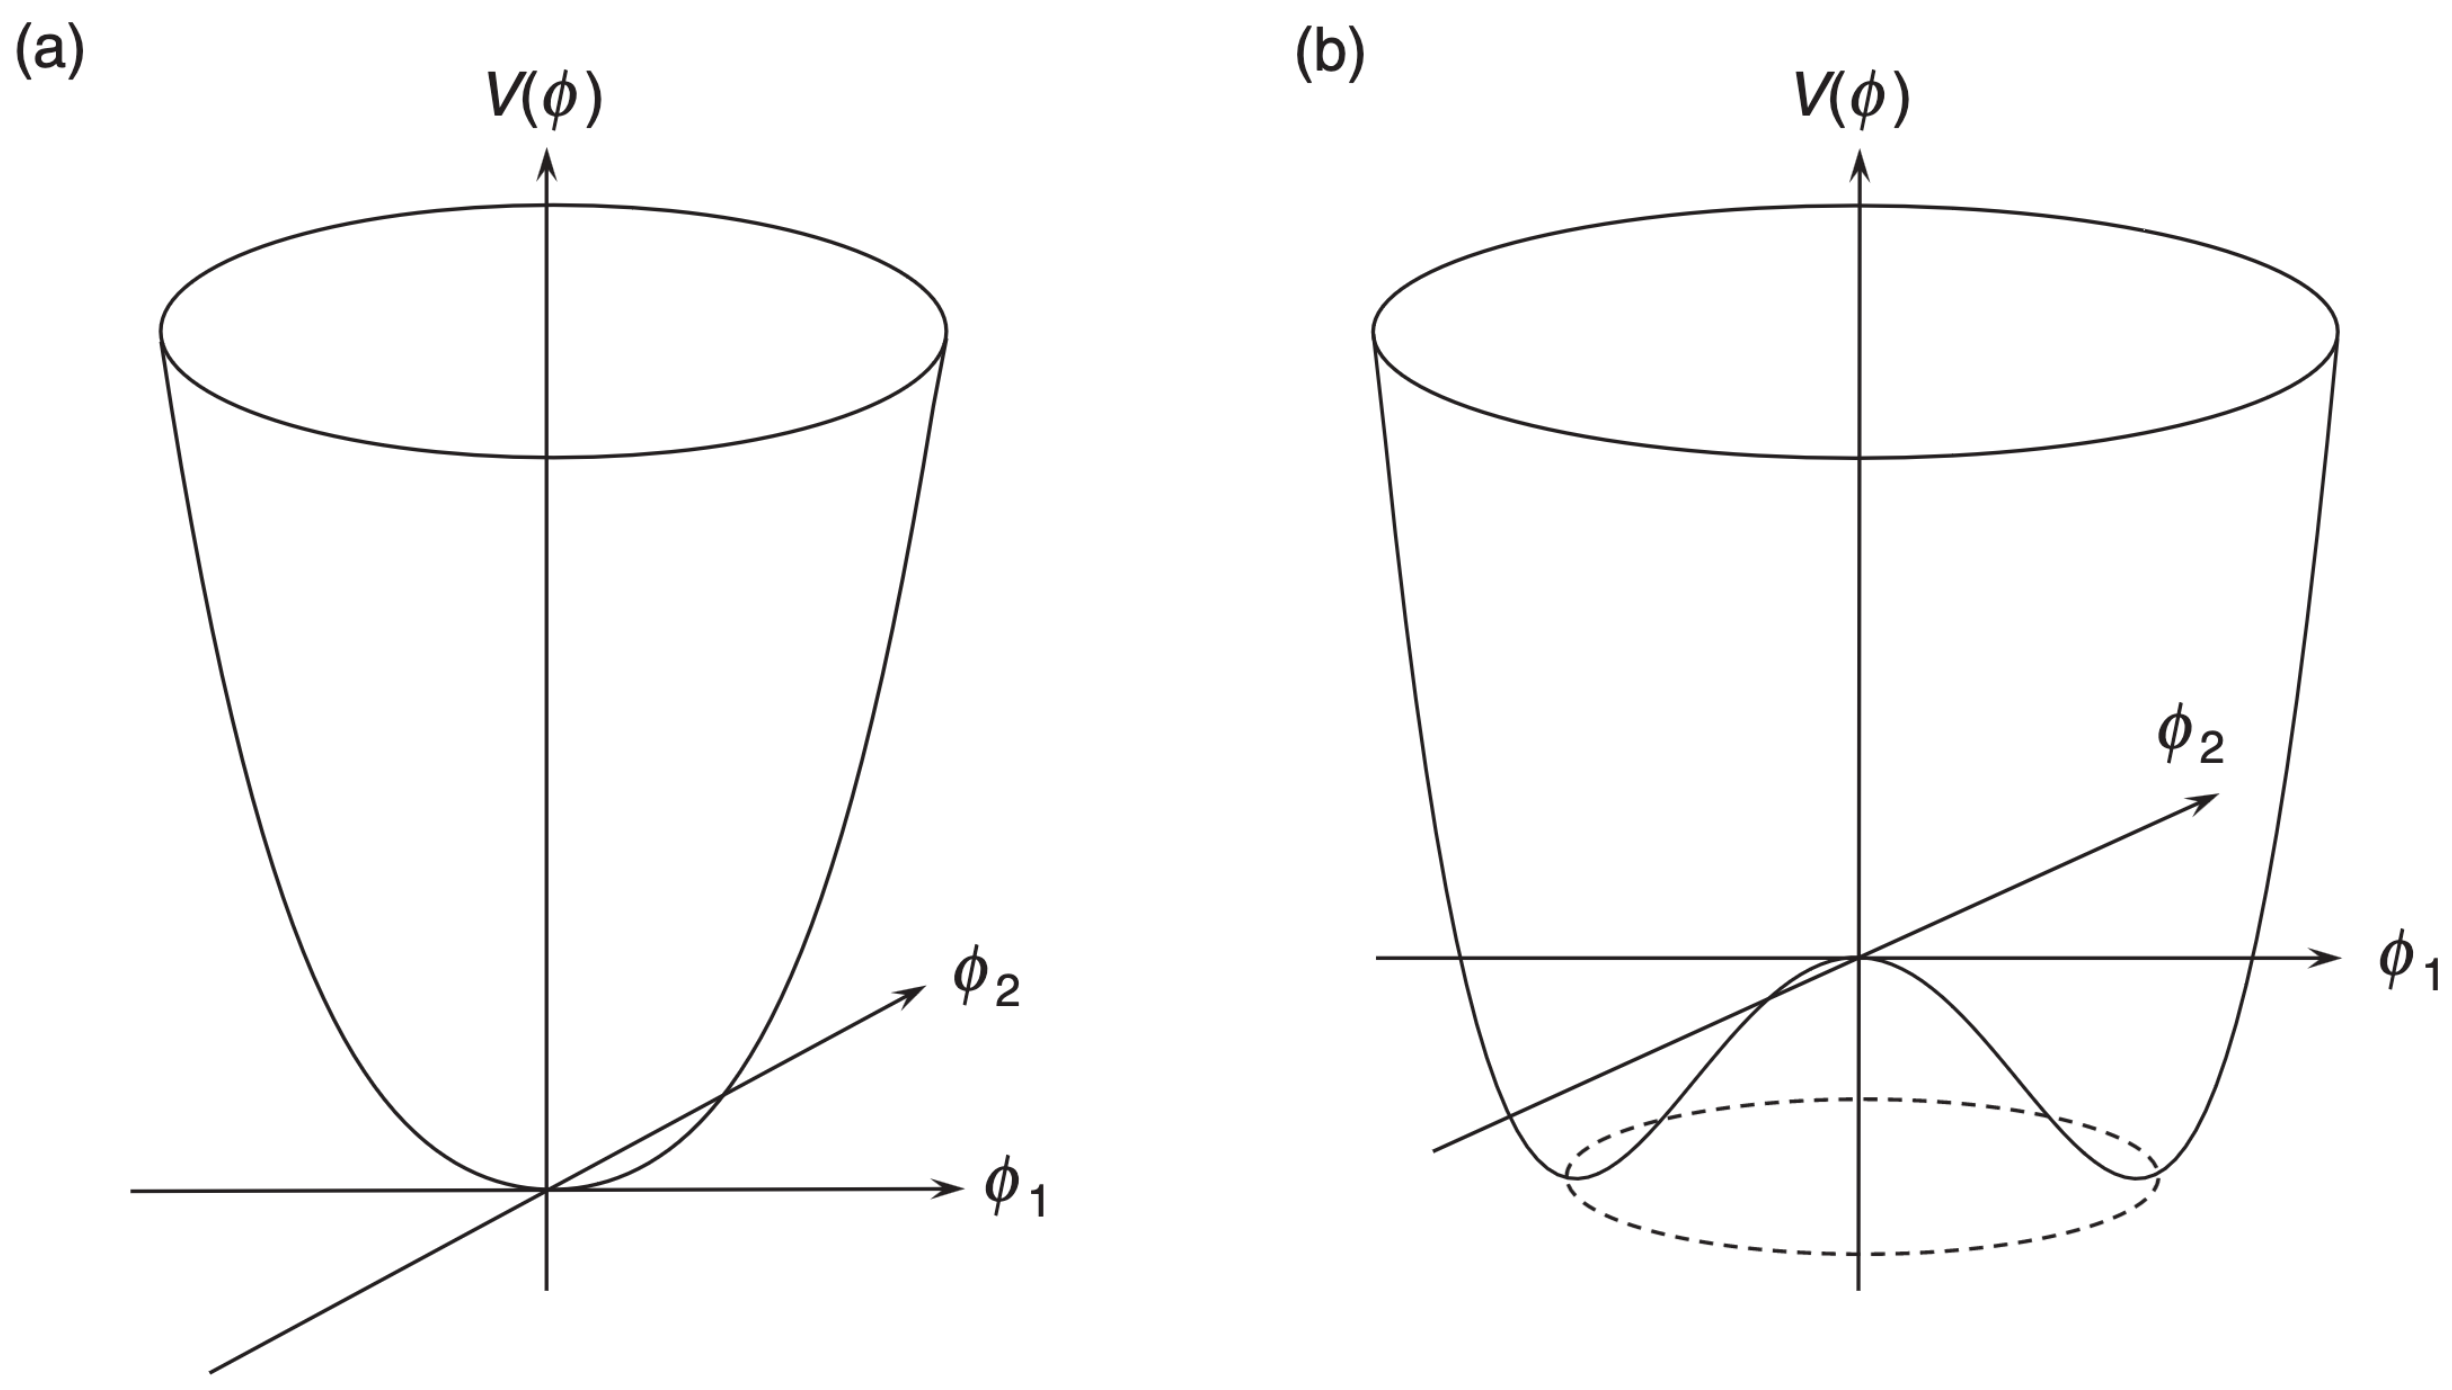
\includegraphics[width=.8\textwidth]{higgs_potential}
    \caption[]{Potential $V(\phi)$: (\textbf{a}) for $\lambda>0$ and $\mu^2<0$ and (\textbf{b}) for values $\lambda>0$ and $\mu^2>0$. Adopted from \citep{thomson2013modern}.}
    \label{fig:higgs_potential}
\end{figure}

The \ac{qft} perturbation ansatz from section \ref{sec:qft} starts from perturbations around the ground state. Thus for the ansatz to work with the $\mu^2>0$ case new field variables $\eta(x)$ and $\xi(x)$ can be introduced so the perturbation calculus can be applied about the ground state
\begin{equation}
    \phi_1(x)=v+\eta(x),\quad \phi_2(x)=\xi(x).
\end{equation}
The physical vacuum state spontaneously breaks the symmetry of the Lagrangian. Furthermore the physical predictions of the Lagrangian do not depend on the choice of the gauge and can be chosen in a way that it eliminates the field $\xi (x)$. In particular, if $\alpha(x)=-\xi(x)/(gv)$, the transformation from equation \ref{eq:scalar_local_gauge} can be made unitary ($UU^\dagger=1$) when expressed to first order in the field variables. Moreover $\eta(x)$ can then be reinterpreted as a Higgs field $h(x)$
\begin{equation}
    \phi(x)  \rightarrow  e^{i g\alpha(x)}\frac{1}{\sqrt{2}}(v+\eta(x)+i\xi(x))
    \approx
    \frac{1}{\sqrt{2}}e^{-i \frac{\xi(x)}{v}}[v+\eta(x)]e^{i\frac{\xi(x)}{v}}
    =
    \frac{1}{\sqrt{2}}(v+h(x)).
\end{equation}
The full local gauge invariant Lagrangian for a $U(1)$ complex scalar field then reads except for constants
\begin{align}
    \mathcal{L}= &
    \underbrace{\frac{1}{2}(\partial_\mu h)(\partial^\mu h)-\lambda v^2 h^2}_{\text{massive h scalar}}
    -
    \underbrace{\frac{1}{4}F_{\mu\nu}F^{\mu\nu} -\frac{1}{2}g^2v^2 B_\mu B^\mu}_{\text{massive boson}}
    \nonumber
    \\
                 & + \underbrace{g^2vB_\mu B^\mu h+\frac{1}{2}g^2 B_\mu B^\mu h^2}_{\text{h,B interactions}}
    -
    \underbrace{\lambda v h^3 -\frac{1}{4}\lambda h^4}_{\text{h self-interactions}},
\end{align}
and describes a massive scalar particle $h$, a massive boson $B_\mu$, interactions between the scalar and boson and as well interactions of the scalar itself depicted in figure \ref{fig:higgs_couplings}.
\begin{figure}
    \centering
    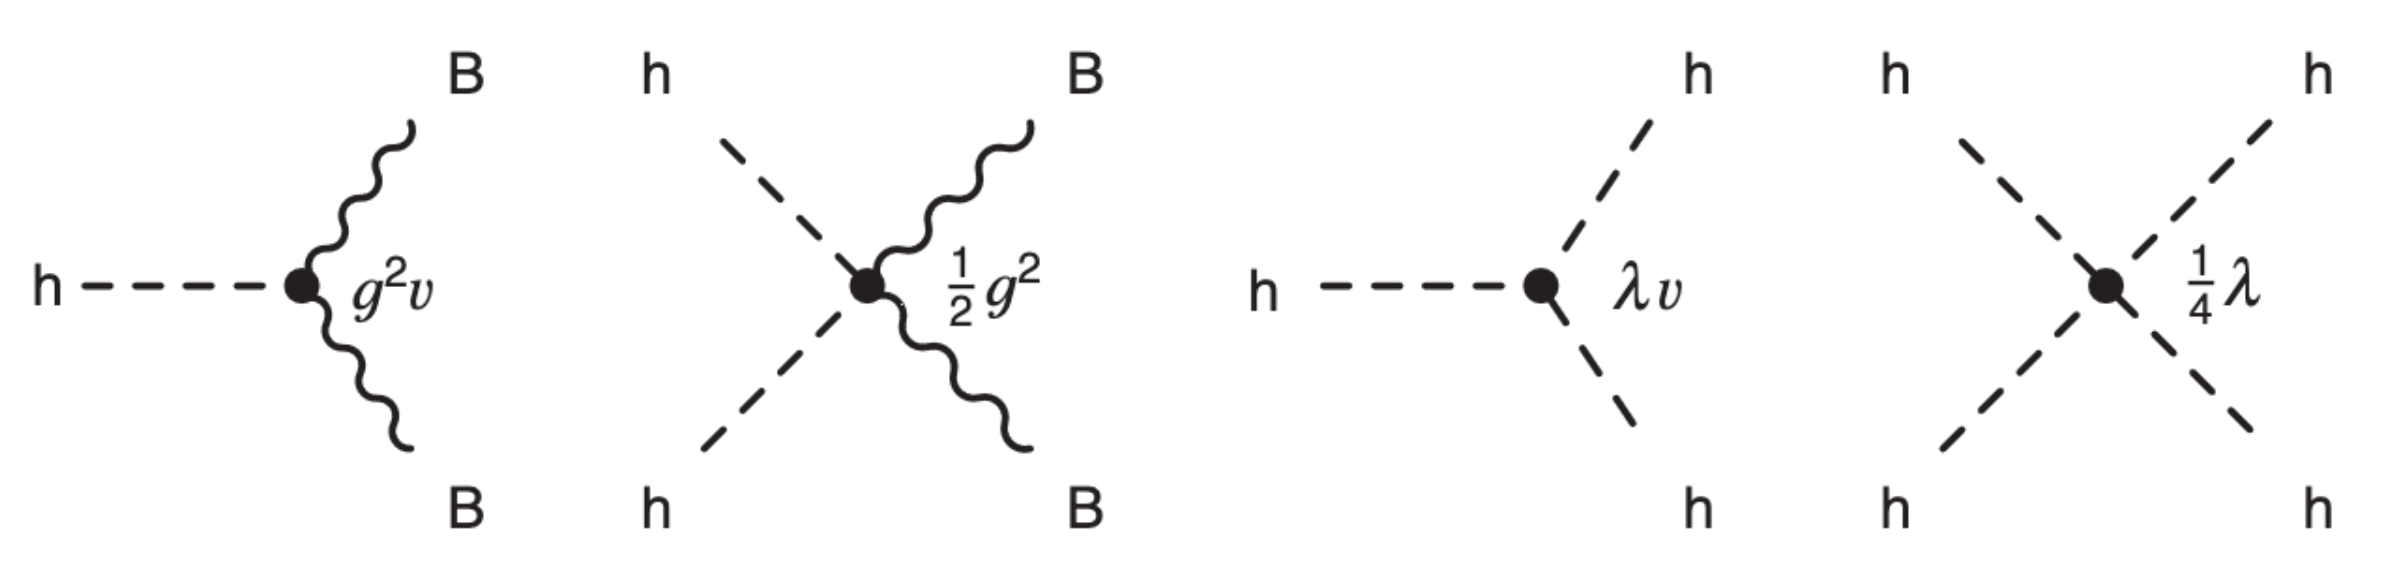
\includegraphics[width=.8\textwidth]{higgs_couplings}
    \caption[]{Self-interactions of a Higgs from a local $U(1)$ gauge symmetry. Adopted from \citep{thomson2013modern}.}
    \label{fig:higgs_couplings}
\end{figure}

\subsection*{The Standard Model Higgs}
For the electroweak Lagrangian the $SU(2)_L \otimes U(1)_Y$ symmetry is broken by the Higgs mechanism while maintaining the electromagnetic $U(1)_{EM}$ symmetry. This is also called \ac{ewsb} and is realized with a isospin doublet of complex scalar fields
\begin{equation}
    \phi(x)=
    \begin{pmatrix}
        \phi^+(x) \\
        \phi^0(x)
    \end{pmatrix}
    =
    \begin{pmatrix}
        \phi_1 (x)+i \phi_2 (x) \\
        \phi_3 (x)+i \phi_4 (x)
    \end{pmatrix}.
\end{equation}
with weak hyperchage $Y=1$. The upper state $\phi^+$ with $I_3=1/2$ is electrically charged and the lower state $\phi^0$ with $I_3=-1/2$ is electrically neutral consistent with the Gell-Mann Nishijima formula from equation \ref{eq:gellmann_nishijima_formula}.


\subsubsection*{Higgs Term}
With $Y=1$ the covariant derivative from equation \ref{eq:cov_diff_L} becomes
\begin{equation}
    D_\mu=\partial_\mu- i g_2\frac{{\sigma}_a}{2}W_\mu^a+ ig_1\frac{1}{2}B_\mu.
\end{equation}
and the Higgs term for the electroweak Lagrangian of equation \ref{eq:L_EW} is
\begin{equation}
    \mathcal{L}_\text{Higgs}= \left(D_\mu\phi\right)^\dagger (D^\mu\phi)-V(\phi),
    \label{eq:L_higgs}
\end{equation}
with the Higgs potential
\begin{equation}
    V(\phi) = -\mu^2\phi^\dagger\phi+\frac{\lambda}{4}\left(\phi^\dagger\phi\right)^2.
    \label{eq:Higgs_initial_potential}
\end{equation}
In analogy to the steps for the $U(1)$ Higgs mechanism from section \ref{sec:higgs_mechanism} there is a set of degenerate minima for $\mu^2,\lambda>0$
\begin{equation}
    \phi^\dagger\phi=\frac{1}{2}(\phi_1^2+\phi_2^2+\phi_3^2+\phi_4^2)=\frac{v^2}{2}=\frac{4\mu^2}{\lambda}.
    \label{eq:higgs_vev}
\end{equation}
Since the photon needs to remain massless and as shown in section \ref{sec:higgs_mechanism} broken symmetries generate gauge bosons with mass, the \ac{vev} is chosen in a way that the vacuum shares the symmetry of the electromagnetic gauge group $U(1)_{EM}$ from section \ref{sec:qed} via setting \mbox{$\phi_1=\phi_2=\phi_4=0$} and $\phi_3=v$ such that the \ac{vev} becomes
\begin{equation}
    \langle0\vert \phi \vert0\rangle=\phi_0=\frac{1}{\sqrt{2}}
    \begin{pmatrix}
        0 \\
        v
    \end{pmatrix}.
\end{equation}
The generator of the electromagnetic subgroup is $Q=I_3+Y/2$. $\phi_0$ breaks $SU(2)_L$ and $U(1)_Y$ but since the lower state is electrically neutral $Q=0$, it remains local gauge invariant under $U(1)_{EM}$ as can be seen from
\begin{equation}
    \phi_0 \rightarrow e^{i\alpha(x)Q}\phi_0=\phi_0.
\end{equation}
Expanding the field about the \ac{vev}
\begin{equation}
    \phi(x)=\frac{1}{\sqrt{2}}
    \begin{pmatrix}
        \phi_1 (x)+i \phi_2 (x) \\
        v+ \eta(x)+i \phi_4 (x)
    \end{pmatrix},
\end{equation}
becomes in the unitary gauge with the physical \ac{sm} Higgs field $h$
\begin{equation}
    \phi(x)=\frac{1}{\sqrt{2}}
    \begin{pmatrix}
        0 \\
        v+h(x)
    \end{pmatrix}.
    \label{eq:unitary_gauge}
\end{equation}
In this form the potential then becomes with equation \ref{eq:higgs_vev} in terms of $\mu$ and $v$
\begin{equation}
    V=\mu^2h^2+\frac{\mu^2}{v}h^3+\frac{\mu^2}{4v^2}h^4
    =
    \frac{m_h^2}{2}h^2+\frac{m_h^2}{2v}h^3+\frac{m_h^2}{8v^2}h^4.
    \label{eq:higgs_potential}
\end{equation}
This yields a Higgs mass term $m_h=\mu\sqrt{2}$ and triplet and quartic self-couplings proportional to the Higgs mass. The kinematic term of the Higgs Lagrangian can be brought into a form that the gauge fields $W^1_\mu,W^2_\mu,W^3_\mu,B_\mu$ represent the physical fields: the charged massive $W^{\pm}$ gauge bosons then are
\begin{equation}
    W_\mu^\pm = \frac{1}{\sqrt{2}}(W_\mu^1\mp i W_\mu^2),
\end{equation}
and the neutral massive $Z$ boson and the massless photon $A_\mu$ are mixed states of
\begin{equation}
    \begin{pmatrix}
        A_\mu \\
        Z_\mu
    \end{pmatrix}
    =
    \begin{pmatrix}
        \cos\theta_W  & \sin\theta_W \\
        -\sin\theta_W & \cos\theta_W
    \end{pmatrix}
    \begin{pmatrix}
        B_\mu \\
        W^3_\mu
    \end{pmatrix}
\end{equation}
rotated by the Weinberg weak mixing angle $\theta_W$. The kinematic Higgs term then becomes
\begin{equation}
    \left(D_\mu\phi\right)^\dagger (D^\mu\phi )=
    \frac{1}{2}(\partial_\mu h)(\partial^\mu h)+
    \frac{g_2^2}{4}W^-_\mu W^{+\mu}(v+h)^2+
    \frac{g_1^2+g_2^2}{4} Z_\mu Z^\mu(v+h)^2.
    \label{eq:higgs_kinematic}
\end{equation}
% \begin{align}
%     \left(D_\mu\phi\right)^\dagger (D^\mu\phi )= &
%     \frac{1}{2}(\partial^\mu h)(\partial_\mu h)+
%     \frac{g_2^2}{4}W^-_\mu W^{+\mu}(v+h)^2+
%     \\
%                                                  & \frac{1}{2}\begin{pmatrix}
%                                                                   A_\mu & Z_\mu
%                                                               \end{pmatrix}
%     \begin{pmatrix}
%         m_A^2 & 0     \\
%         0     & m_Z^2
%     \end{pmatrix}
%     \begin{pmatrix}
%         A_\mu \\
%         Z_\mu
%     \end{pmatrix}
% \end{align}
and describes trilinear $HWW,HZZ$ and quadrilinear $HHWW,HHZZ$ vertices. The photon becomes naturally massless in this form and the masses of the massive gauge bosons can be read off
\begin{equation}
    m_W= \frac{1}{2}g_2v,\quad m_Z=\frac{1}{2}\sqrt{g_1^2+g_2^2}.
\end{equation}
Furthermore a relation to the weak mixing angle and the electric charge follow
\begin{equation}
    \cos\theta_W=\frac{g_2}{\sqrt{g_1^2+g_2^2}}=\frac{m_W}{m_Z}, \quad e=g\sin \theta_W.
\end{equation}
The $\cos\theta_W$ was experimentally verifiable before the Higgs discovery and a compelling argument for the Higgs to exist.



\subsubsection*{Yukawa Term}\label{sec:yukawa_term}
Fermion masses can be incorporated into the electroweak Lagrangian of equation \ref{eq:L_EW} with the help of the Higgs mechanism in the form of Yukawa couplings. For one generation of leptons and quarks gauge invariant terms are introduced via couplings between the left-handed doublet states, the Higgs field and right handed singlet states
\begin{align}
    \mathcal{L}_\mathrm{Y}^{\text{one gen}} & =
    - \; G_e
    \begin{pmatrix}
        \overline{\nu}_e & \overline{e} \\
    \end{pmatrix}_L
    \begin{pmatrix}
        \phi^+ \\
        \phi^0
    \end{pmatrix}
    e_R                                                                                                                                                                \\
                                            & \phantom{-\;}-G_d
    \begin{pmatrix}
        \overline{u} & \overline{d} \\
    \end{pmatrix}_L
    \begin{pmatrix}
        \phi^+ \\
        \phi^0
    \end{pmatrix}
    d_R                                                                                                                                                                \\
                                            & \phantom{-\;}-G_u
    \begin{pmatrix}
        \overline{u} & \overline{d} \\
    \end{pmatrix}_L
    \begin{pmatrix}
        \phi^{0*} \\
        -\phi^-
    \end{pmatrix}
    u_R                                                                                                                                                                \\
                                            & \phantom{-\;} +h.c.                                                                                                      \\
                                            & = -G_e \overline{L}_L \phi e_R -G_d \overline{Q}_L \phi d_R -G_u \overline{Q}_L \phi_c e_R + h.c. \label{eq:L_Y_one_gen}
\end{align}
with Yukawa coupling constant $G_e,G_d,G_u$ and the charge conjugated Higgs field $\phi_c=i\sigma_2\phi$. The latter can be used because it transforms just like the Higgs field and therefore leaves the Lagrangian gauge invariant. In the unitary gauge mass terms arise e.g. for the electron in the form
\begin{equation}
    \mathcal{L}_\mathrm{Y}^e=\frac{-G_e}{\sqrt{2}} v (\overline{e}_L e_R+\overline{e}_R e_L)+\frac{-G_e}{\sqrt{2}} h (\overline{e}_L e_R+\overline{e}_R e_L).
\end{equation}
The mass of a fermion $f$ is therefore
\begin{equation}
    m_f=G_f\frac{v}{\sqrt{2}},
\end{equation}
so that the full Yukawa Lagrangian can be written as
\begin{equation}
    \mathcal{L}_\mathrm{Yukawa}=-\sum_f m_f\overline{\psi}_f \psi_f -\sum_f \frac{m_f}{v}\overline{\psi}_f \psi_f h.
    \label{eq:yukawa_term}
\end{equation}
Consequently the Higgs couples to fermions proportional to their masses. Since physically observed states are mixed states of the $\psi_f$ eigenstates for the charged weak interactions, the formalism can be extended by making the Yukawa couplings $3\times 3$ matrices $G_u=G_{ij}^d$ with $i=u,c,t$ going over up type quarks and $j=d,s,b$ over down type quarks. Thus the quark part of the Yukawa Lagrangian of equation \ref{eq:L_Y_one_gen} becomes
\begin{equation}
    \mathcal{L}_\mathrm{Y}^{\text{quarks}} =
    -G_{ij}^d \overline{Q}_L^i \phi d_R^j -G_{ij}^u \overline{Q}_L^i \phi_c e_R^j + h.c.
\end{equation}
The $G_{ij}$ matrices mix the eigenstates and can be diagonalized with four unitary matrices $V_{L,R}^{u,d}$
\begin{equation}
    \Tilde{u}^i_{L,R}=(V^u_{L,R})_{ik}u^k_{L,R}, \quad \Tilde{d}^i_{L,R}=(V^d_{L,R})_{ik}u^k_{L,R}.
\end{equation}
With the identity $V_L^uV_L^{d\dagger}\equiv V_\mathrm{CKM}$ the quark mixing matrix also called \acf{ckm} matrix mixes the physical quark eigenstates
\begin{equation}
    \begin{pmatrix}
        d' \\
        s' \\
        b' \\
    \end{pmatrix}
    =V_\mathrm{CKM}\begin{pmatrix}
        d \\
        s \\
        b \\
    \end{pmatrix}=
    \begin{pmatrix}
        V_{ud} & V_{us} & V_{ub} \\
        V_{cd} & V_{cs} & V_{cb} \\
        V_{td} & V_{ts} & V_{tb} \\
    \end{pmatrix}
    \begin{pmatrix}
        d \\
        s \\
        b \\
    \end{pmatrix}.
\end{equation}
The $V_{ij}$ describes the transition probability for a quark $j$ to quark $i$ via the charged weak interactions. In this model neutrinos are assumed to be massless. While it is theoretically possible to incorporate neutrino masses into the \ac{sm}, the mechanism for doing so remains unclear. Introducing neutrino mass terms in a manner similar to that of up-type quarks requires to introduce right-handed neutrinos, which have not been observed. This completes the current \ac{sm} electroweak Lagrangian of equation \ref{eq:L_EW}.

\section{Renormalization}\label{sec:renormalization}
\begin{figure}
    \centering
    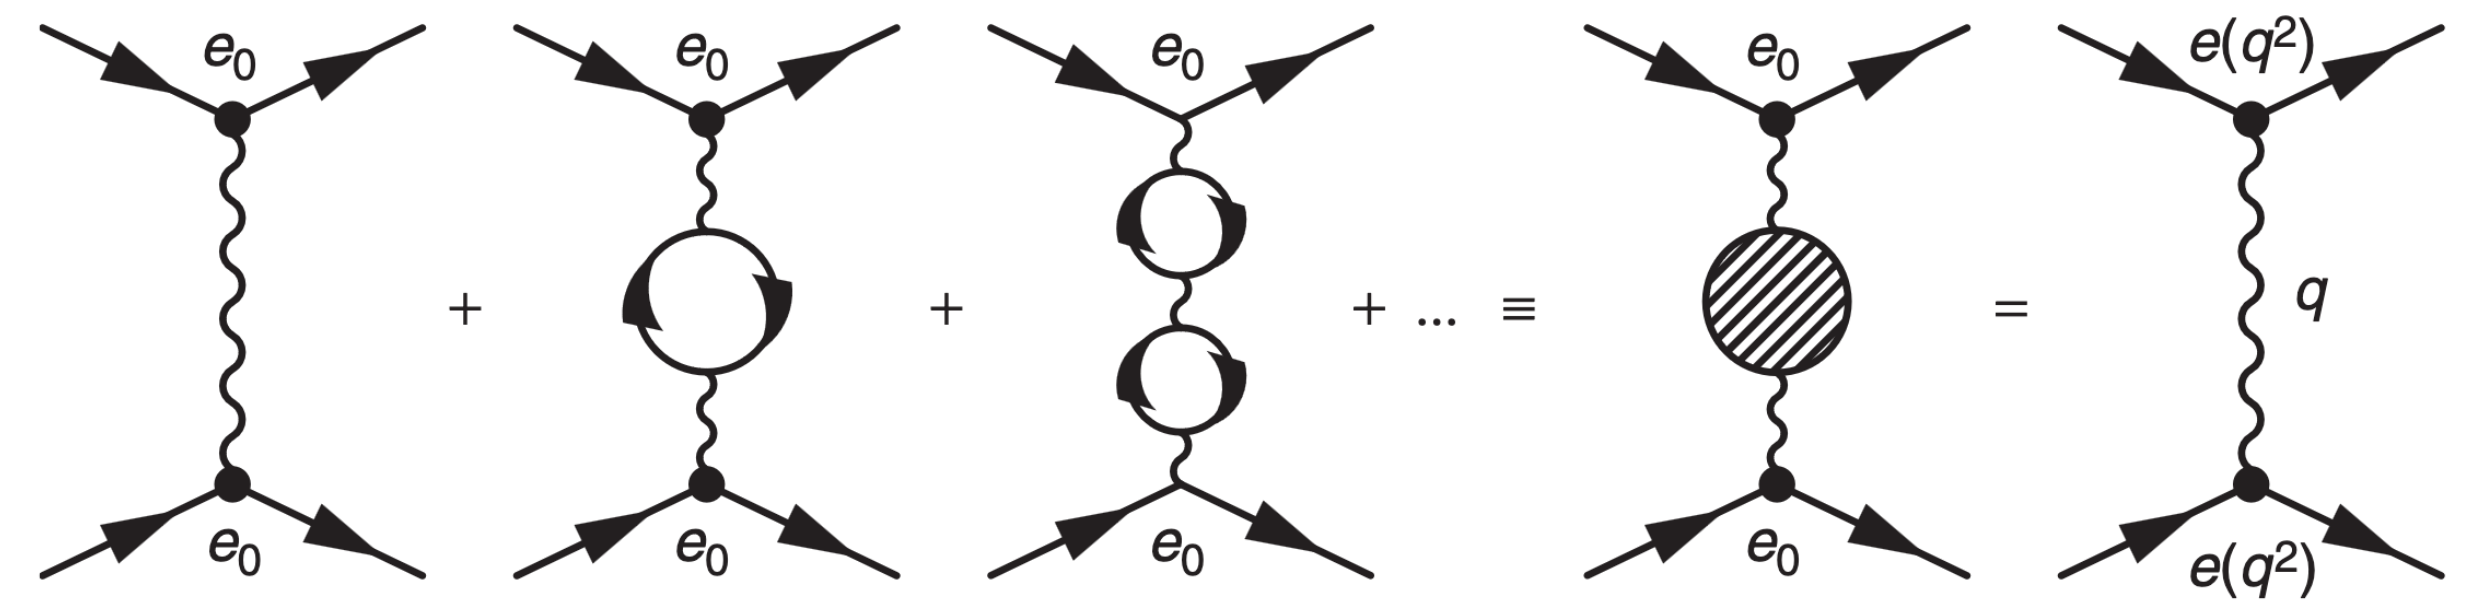
\includegraphics[width=1\textwidth]{qed_diagrams}
    \caption[]{Higher order loop corrections in \ac{qed} schematically treated as one effective diagram. Adopted from \citep{thomson2013modern}.}
    \label{fig:qed_diagrams}
\end{figure}
When attempting to calculate amplitudes $\mathcal{M}$ for higher-order diagrams in \ac{qed}, such as the second or third diagrams shown in Figure \ref{fig:qed_diagrams}, it results in diverging integrals. This phenomenon, known as vacuum polarization, occurs as virtual particle-antiparticle pairs act to screen the actual charge of the electron $e_0$, analogous to a dielectric medium in classical electrodynamics. To address this issue, an effective charge/coupling $e(q^2)$ is introduced. This coupling becomes a function of the squared four-momentum $q^2$ at the virtual photon vertex, as depicted in Figure \ref{fig:qed_diagrams} and renders the integrals finite.

For the second diagram in figure \ref{fig:qed_diagrams} with only one loop correction, it can be shown that for some measured coupling $e(q^2=\mu^2)$ at an energy scale $\mu^2$, the actual coupling $e(q^2)$ follows a scaling behavior that holds if $q^2$ and $\mu^2$ are larger than the electron mass \citep{thomson2013modern}. The coupling constant is now a running coupling $e(q^2)$ and reads in terms of the fine structure constant $\alpha(q^2)=e^2(q^2)/4\pi$,
\begin{equation}
    \alpha(q^2)=
    \frac{\alpha(\mu^2)}
    {1-\alpha(\mu)\frac{1}{3\pi}
        \ln
        \left(\frac{q^2}{\mu^2}\right)}.
    \label{eq:qed_coupling}
\end{equation}
Therefore with increasing momentum transfer, or a decreasing distance when colliding particles, the number of virtual pair production processes is effectively reduced, revealing the bare charge of the electron. This behavior is shown qualitatively in figure \ref{fig:renorm_scaling}(a).
\begin{figure}
    \centering
    \subfigure[]{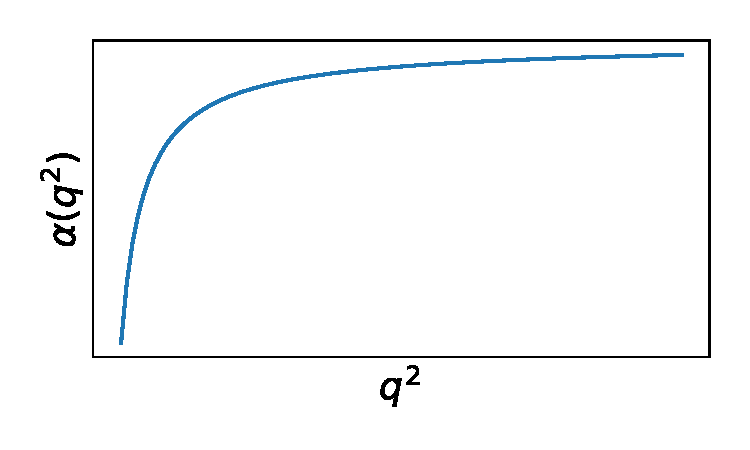
\includegraphics[width=.49\textwidth]{qed_scaling}}
    \subfigure[]{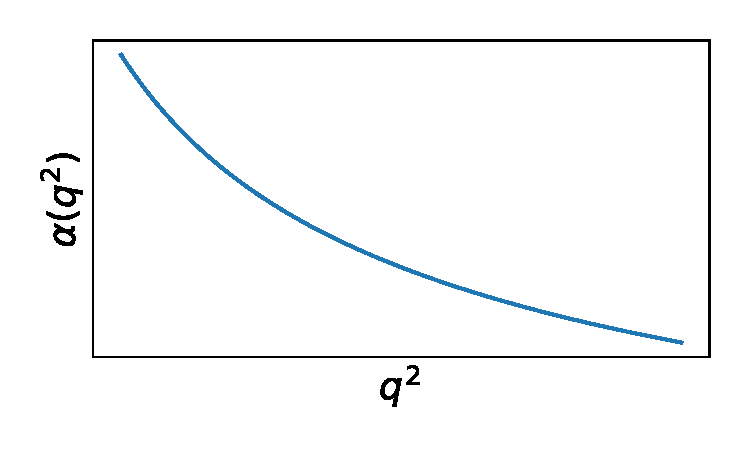
\includegraphics[width=.49\textwidth]{qcd_scaling}}
    \caption[]{Qualitative behavior of the running couplings for (\textbf{a}) \ac{qed} as of equation \ref{eq:qed_coupling} and (\textbf{b}) \ac{qcd} as of equation \ref{eq:qcd_coupling}.}
    \label{fig:renorm_scaling}
\end{figure}
\begin{figure}[H]
    \centering
    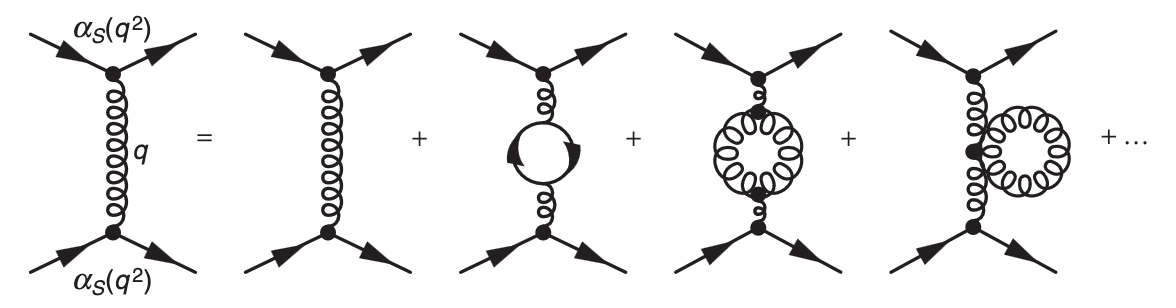
\includegraphics[width=1\textwidth]{qcd_diagrams}
    \caption[]{Some higher order loop corrections in \ac{qcd}. Adopted from \citep{thomson2013modern}.}
    \label{fig:qcd_diagrams}
\end{figure}
Renormalization in \ac{qcd} can be derived similarly but also the quartic and triplet couplings exemplified in figure \ref{fig:qcd_diagrams} need to be considered. This results in a scaling for the strong coupling
\begin{equation}
    \alpha_S(q^2)=
    \frac{\alpha_S(\mu^2)}
    {1+B\alpha_S(\mu)
        \ln
        \left(\frac{q^2}{\mu^2}\right)}, \qquad \text{with } B=\frac{11N_c-2N_f}{12\pi}.
    \label{eq:qcd_coupling}
\end{equation}
For 3 color charges $N_c$ and 6 flavors $N_f$ in the \ac{sm}, $B$ is positive and the coupling becomes weaker for shorter scales or higher momentum transfer as can be seen in figure \ref{fig:renorm_scaling}(b).

The fine structure constant of \ac{qed} $\alpha(q^2\approx 0)\approx 1/137$ does not vary dramatically over the energy ranges of matter for particle physics as shown in figure \ref{fig:renorm_scaling_exp}(a).
\begin{figure}
    \centering
    \subfigure[]{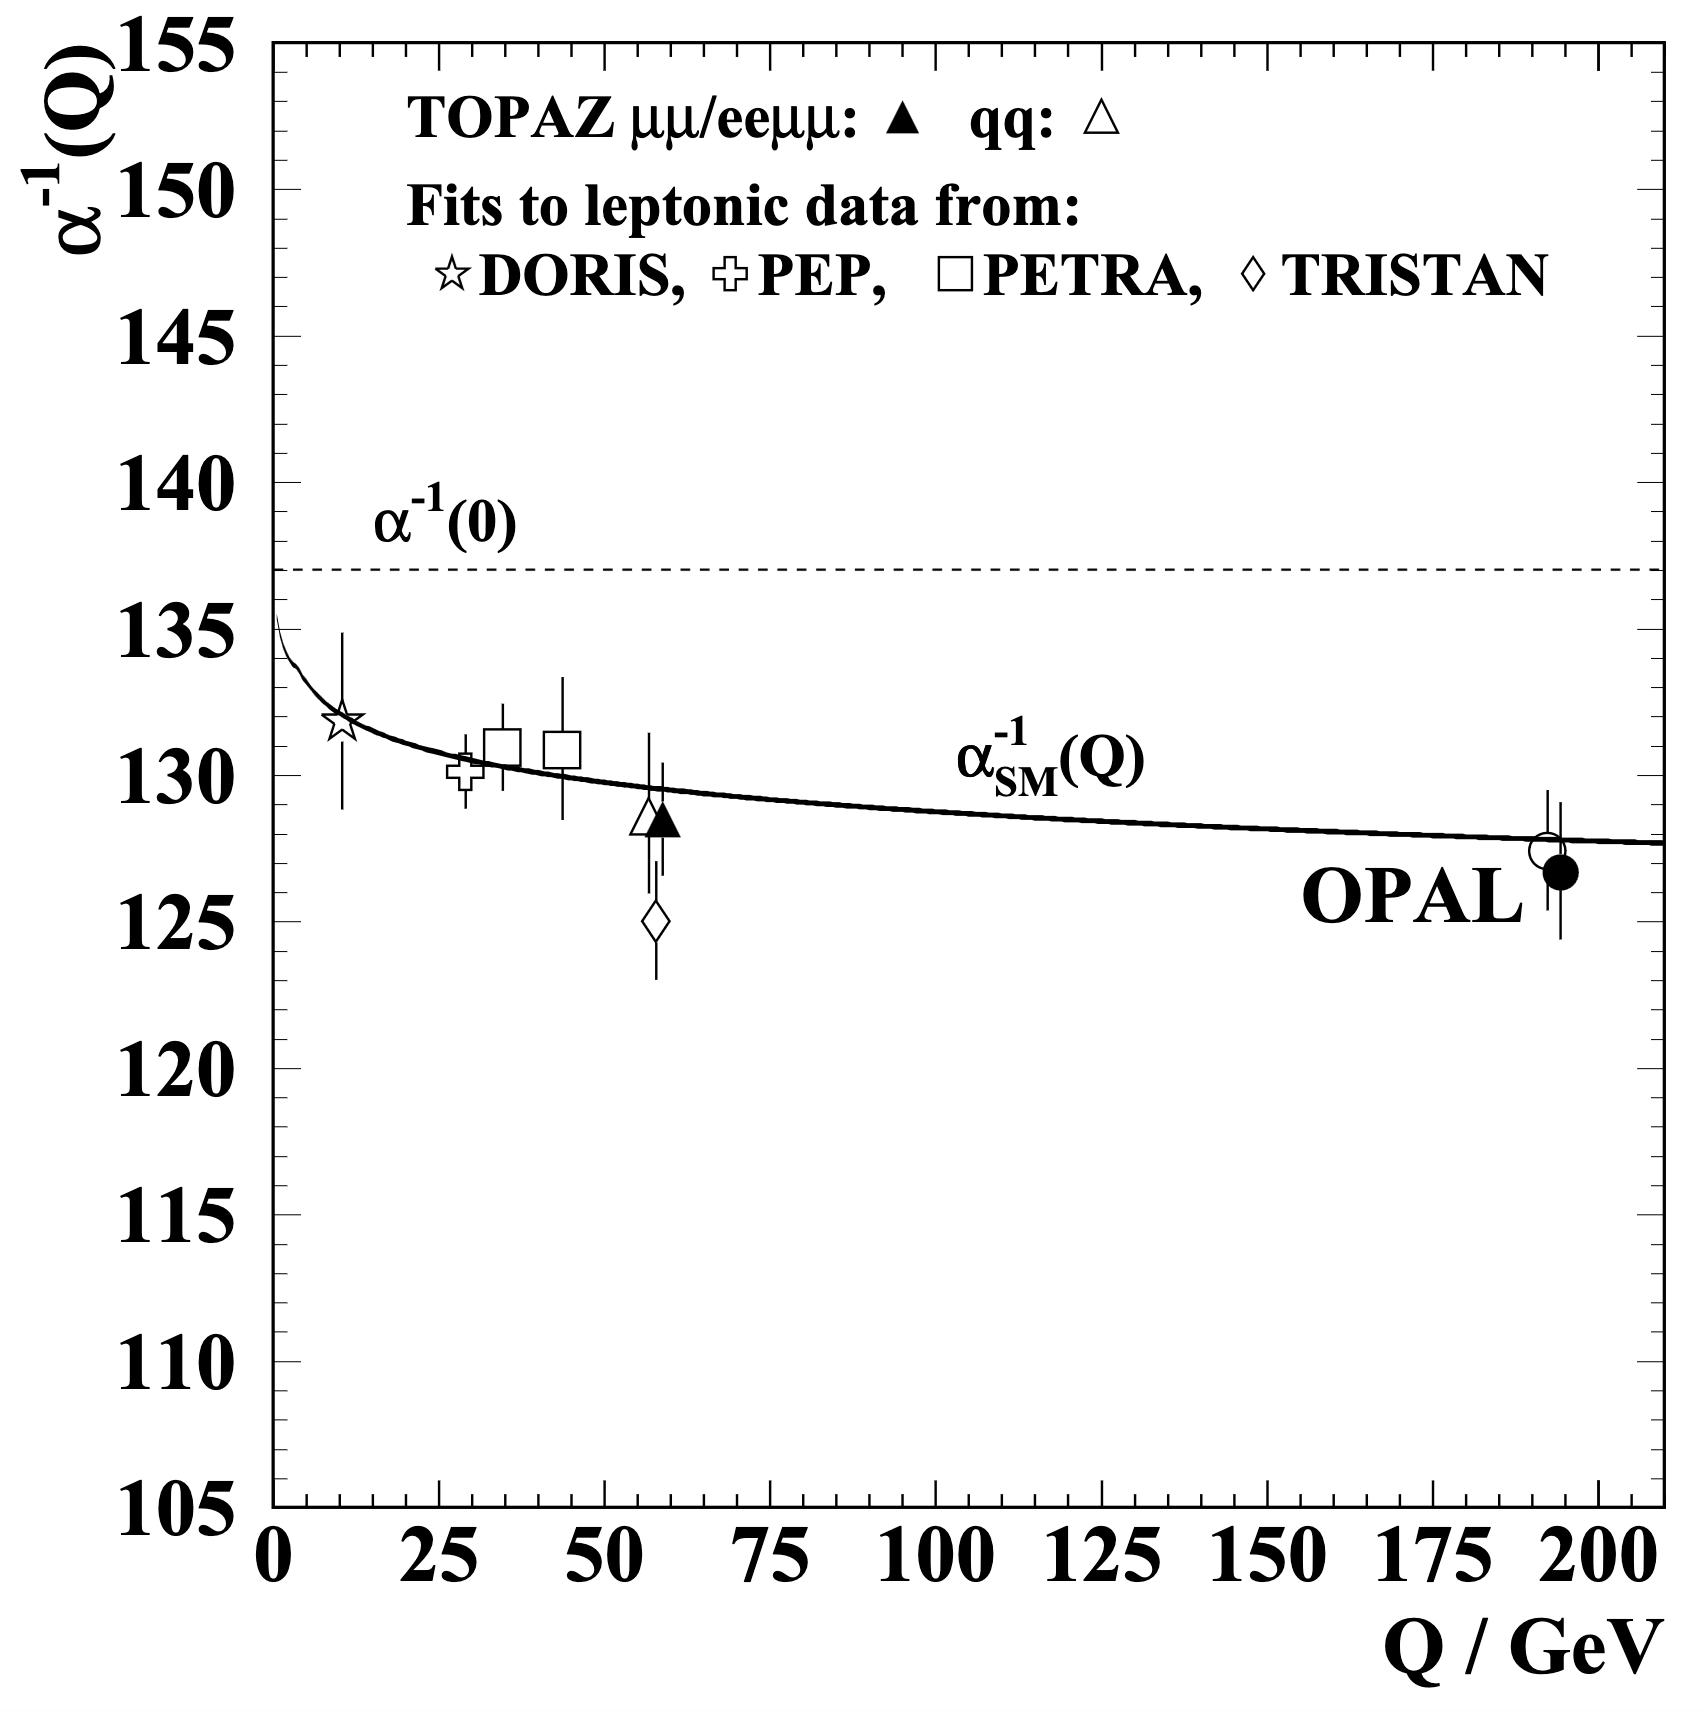
\includegraphics[width=.47\textwidth]{qed_scaling_experiment}}\hspace{5mm}
    \subfigure[]{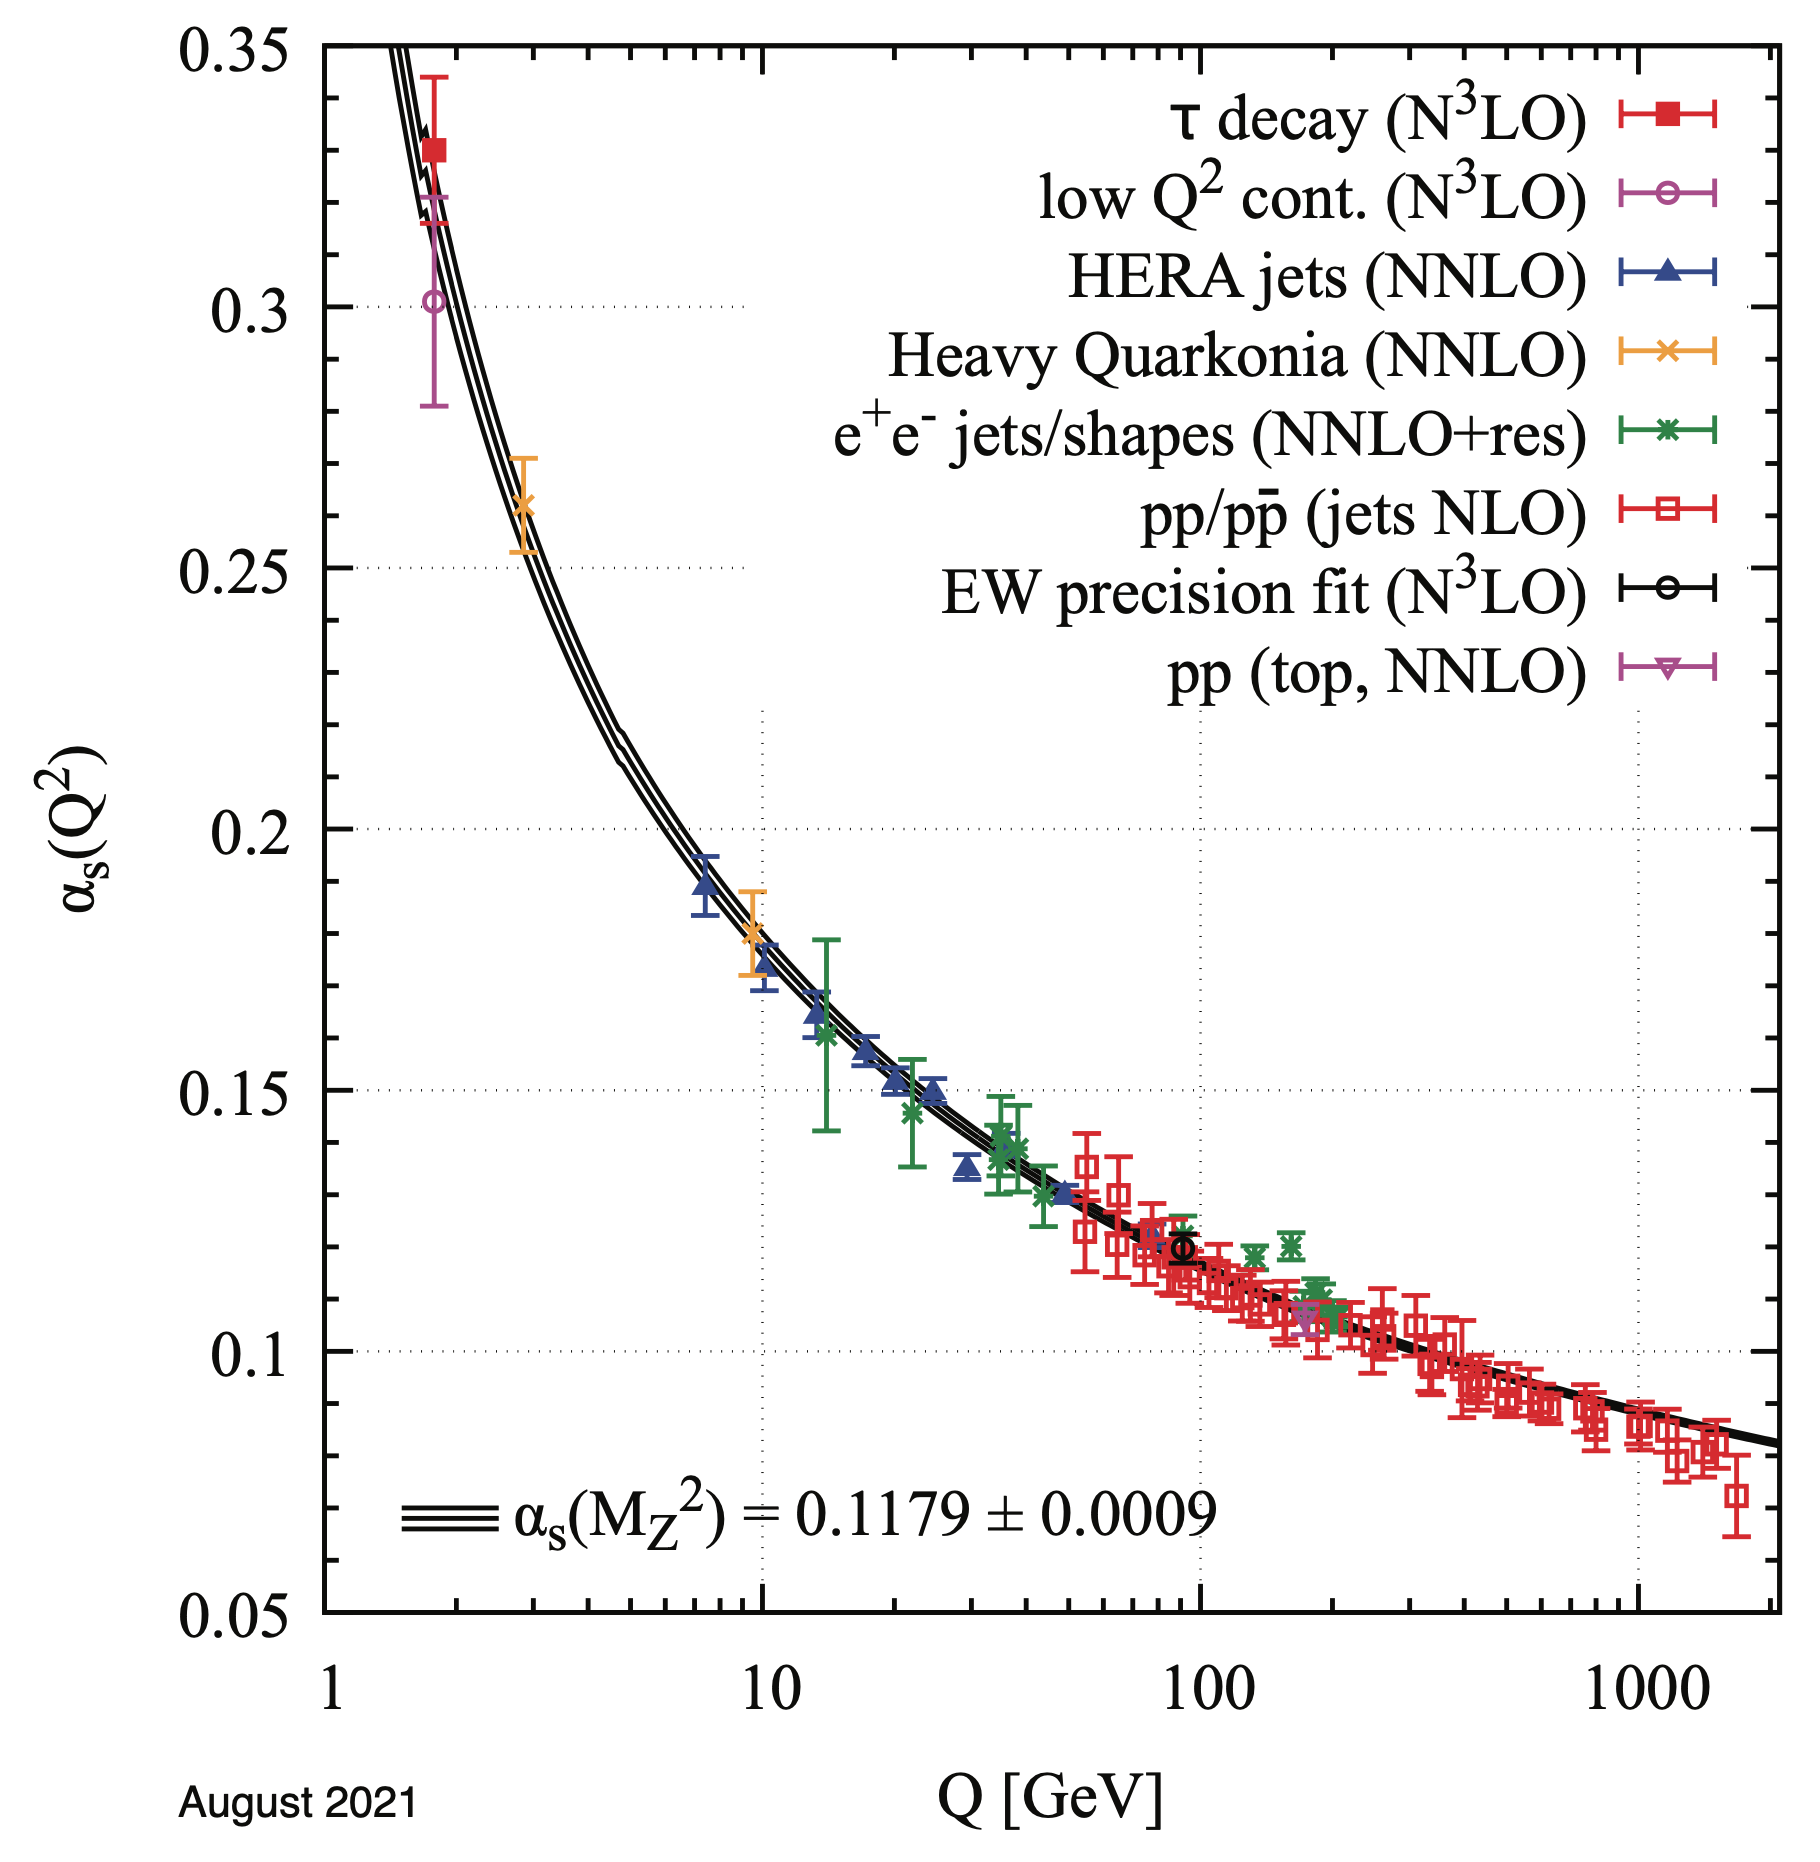
\includegraphics[width=.47\textwidth]{qcd_scaling_experiment}}
    \caption[]{Measurements of the running couplings for (\textbf{a}) \ac{qed} (note the inverted coupling on the y-axis) adopted from \citep{opal2004tests} and (\textbf{b}) \ac{qcd} adopted from \citep{particle2022review}.}
    \label{fig:renorm_scaling_exp}
\end{figure}
Most importantly the running coupling of \ac{qed} does not impact the perturbative approach outlined in section \ref{sec:qft} since $\alpha\ll1$. This is not the case for \ac{qcd} where $\alpha_S$ at $q\approx\qty{1}{GeV}$ is of $\mathcal{O}(1)$. In such scenarios, perturbation theory is ineffective because the expansion in $\alpha_S$ with only one leading term is a poor approximation for calculations of bound hadronic states and later processes in hadronization, as explained below. While perturbation theory for \ac{qcd} remains valid for $\alpha_S\sim  0.1$, which corresponds to $q\gtrsim \qty{100}{GeV}$, for basically all \ac{qcd} calculations at the \ac{lhc}, higher order corrections must be considered.

The behavior of the running coupling in \ac{qcd} is called asymptotic freedom, since the theory is free of asymptotics/divergences with increasing energy scale or decreasing distance. In turn to the photon in \ac{qed}, gluons carry charge and thus attempting to separate quarks results in additional gluons contributions to the interaction, increasing both the energy and force between the quarks. Eventually, it becomes energetically favorable to create a quark-antiquark pair from the vacuum, which then bind with the separating quarks to form new, color-neutral hadrons. This is also known as color confinement, which states that colored particles can only be observed in bound states.

Renormalization is a crucial procedure for ensuring the consistency and predictive power of the \ac{sm} and is also applicable to the electroweak sector. However the complexity of this topic goes beyond the scope of this thesis.


\section{Physics Beyond the Standard Model}\label{sec:beyond_sm}
The \ac{sm} works within its realm but is inherently incomplete given other observed phenomena of which a few are presented here. Most importantly there is no quantum theory for gravity and is thus not part of the \ac{sm}.

Furthermore there is evidence through gravitational effects which cannot be explained by the amounts of ordinary matter which is referred to as dark matter \citep{dark_matter_a_primer}. Furthermore there are several observations showing an accelerated expansion of the universe which is referred to as dark energy \citep{RevModPhys.75.559}. The standard model of cosmology Lambda-Cold Dark Matter ($\Lambda$CDM) \citep{planck2020} models the cosmic microwave background by incorporating dark matter and dark energy with high precision for both of which the \ac{sm} offers no explanation.

Furthermore neutrinos are known to be massive. In principle they can be added like fermions as in the section on the fermion Yukawa mass term \ref{sec:yukawa_term} but this requires right-handed neutrinos which have not been observed. This suggests, since their masses are much smaller than for the other fermions that there might be another mechanism responsible for the generation of the mass of neutrinos.

Moreover, in the standard cosmological model, matter and antimatter should have been created in equal amounts, yet the universe is predominantly made of matter. An explanation of this behavior can be given through the nature of \ac{eswb}. The Sakharov conditions necessary to create the observed baryon asymmetry can be created if \ac{ewsb} is a first order phase transition. In such a transition the position of the minimum in the potential changes abruptly when the universe cools below temperature where \ac{ewsb} occurs as depicted in figure \ref{fig:higgs_phase_transition} \citep{Banerjee2011ElectroweakPT,MICCO2020100045}. 

This phase transition is dictated by the Higgs potential. The assumed form and the measured mass of the \ac{sm} Higgs do not support a first-order phase transition but rather a smooth crossover transition similar to a second order phase transition also shown schematically in figure \ref{fig:higgs_phase_transition} \citep{PhysRevD.105.095041,MICCO2020100045}. The nature of the very early universe is thus inscribed in the shape of the Higgs potential and if we are in an absolute miminum remains unclear as only the mass term of the Higgs potential from equation \ref{eq:higgs_potential} is determined by experiment and only the simplest thinkable potential shape is used to render weak gauges bosons massive. 

\begin{figure}
    \centering
    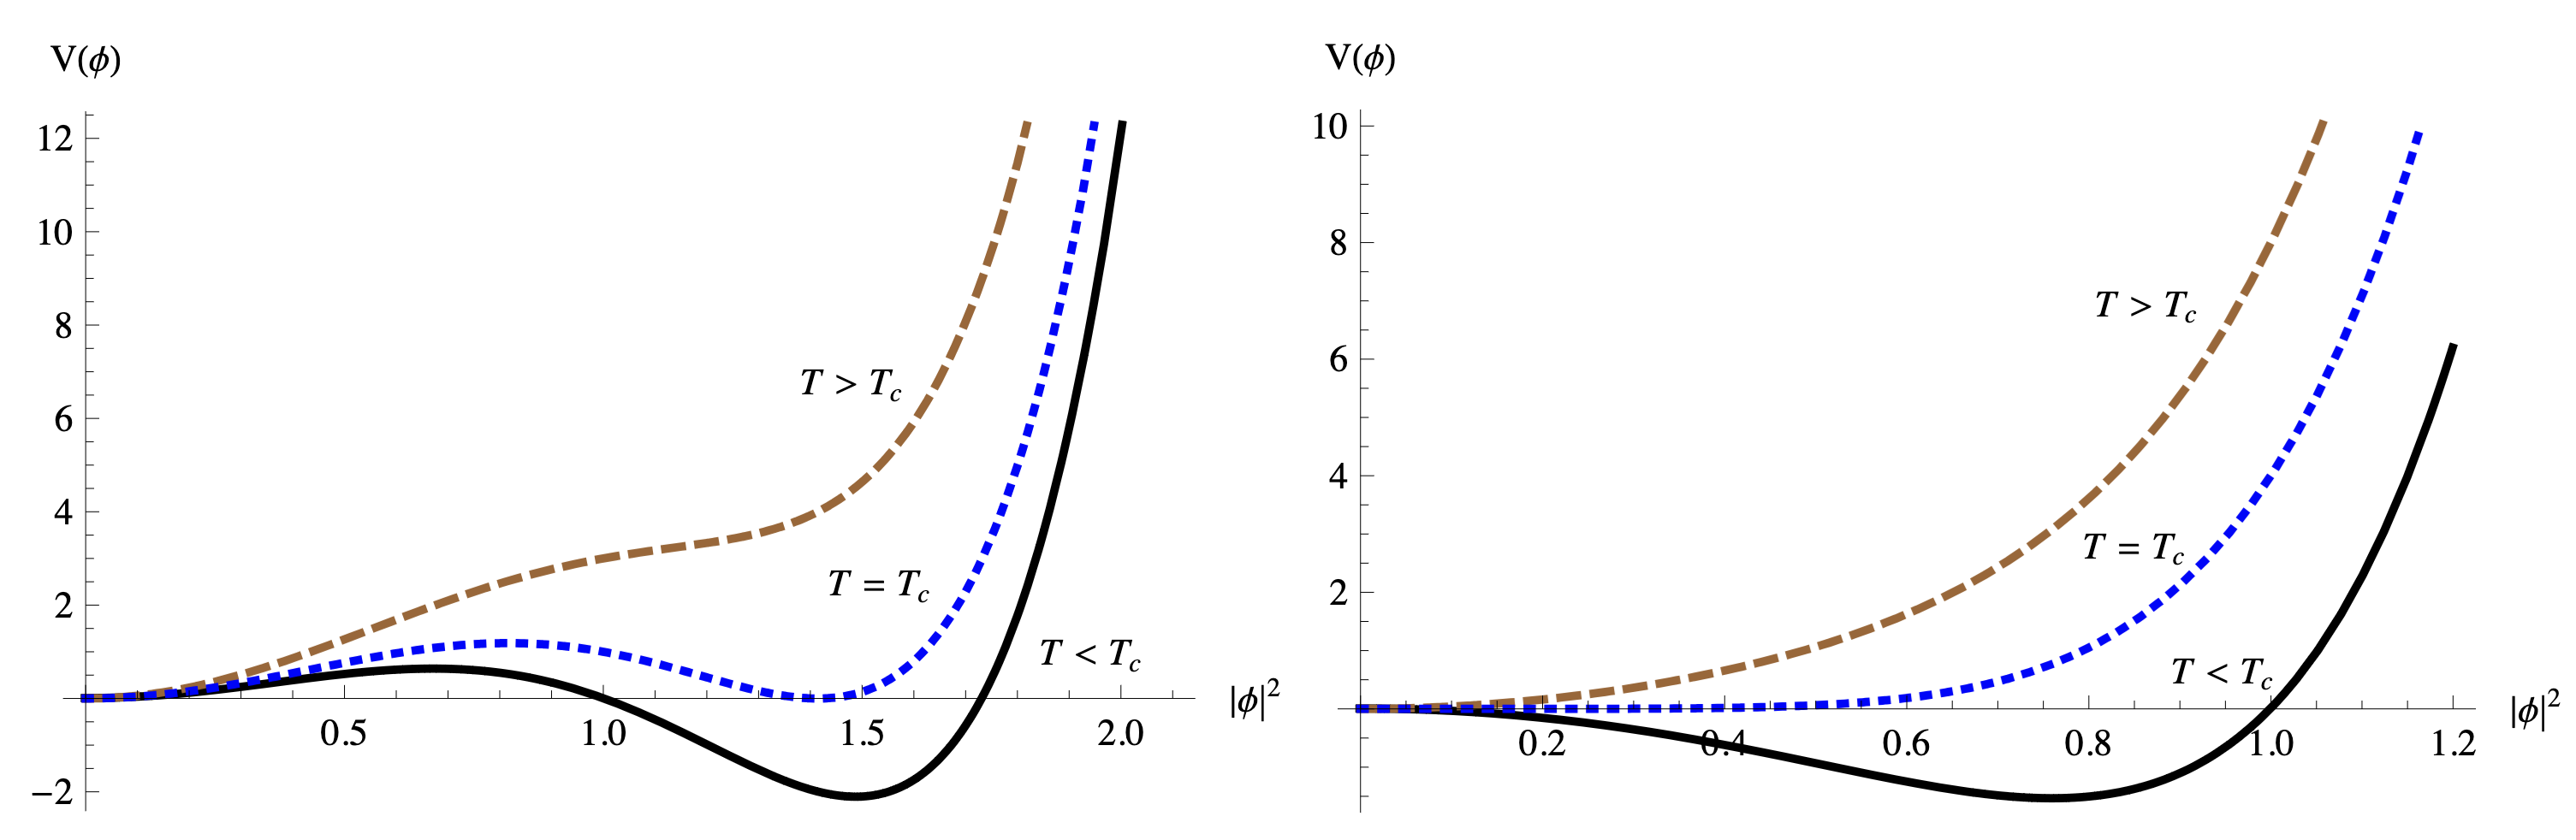
\includegraphics[width=1\textwidth]{higgs_phase_transition}
    \caption[]{(Left) First order phase transition for a given temperature with a sudden change of the minum when the temperature drops below $T_c$, where for (right) a second order phase transition the minimum changes continuously. Adopted from \citep{Banerjee2011ElectroweakPT}.}
    \label{fig:higgs_phase_transition}
\end{figure}

When considering top-quark loop corrections to the Higgs field, as illustrated in figure \ref{fig:top_loop}, the $\lambda(\mu)$ parameter in the Higgs potential becomes energy scale-dependent and allows to make some statements about the shape of the Higgs potential. At an instability energy scale of $\Lambda_I\approx \qty[]{e10}{GeV}$, $\lambda(\mu)$ could turn negative, suggesting that the current \ac{vev} might not be the absolute minimum of the Higgs potential but could be energetically lower or even unbounded \citep{devoto2022false}.


\begin{figure}
    \centering
    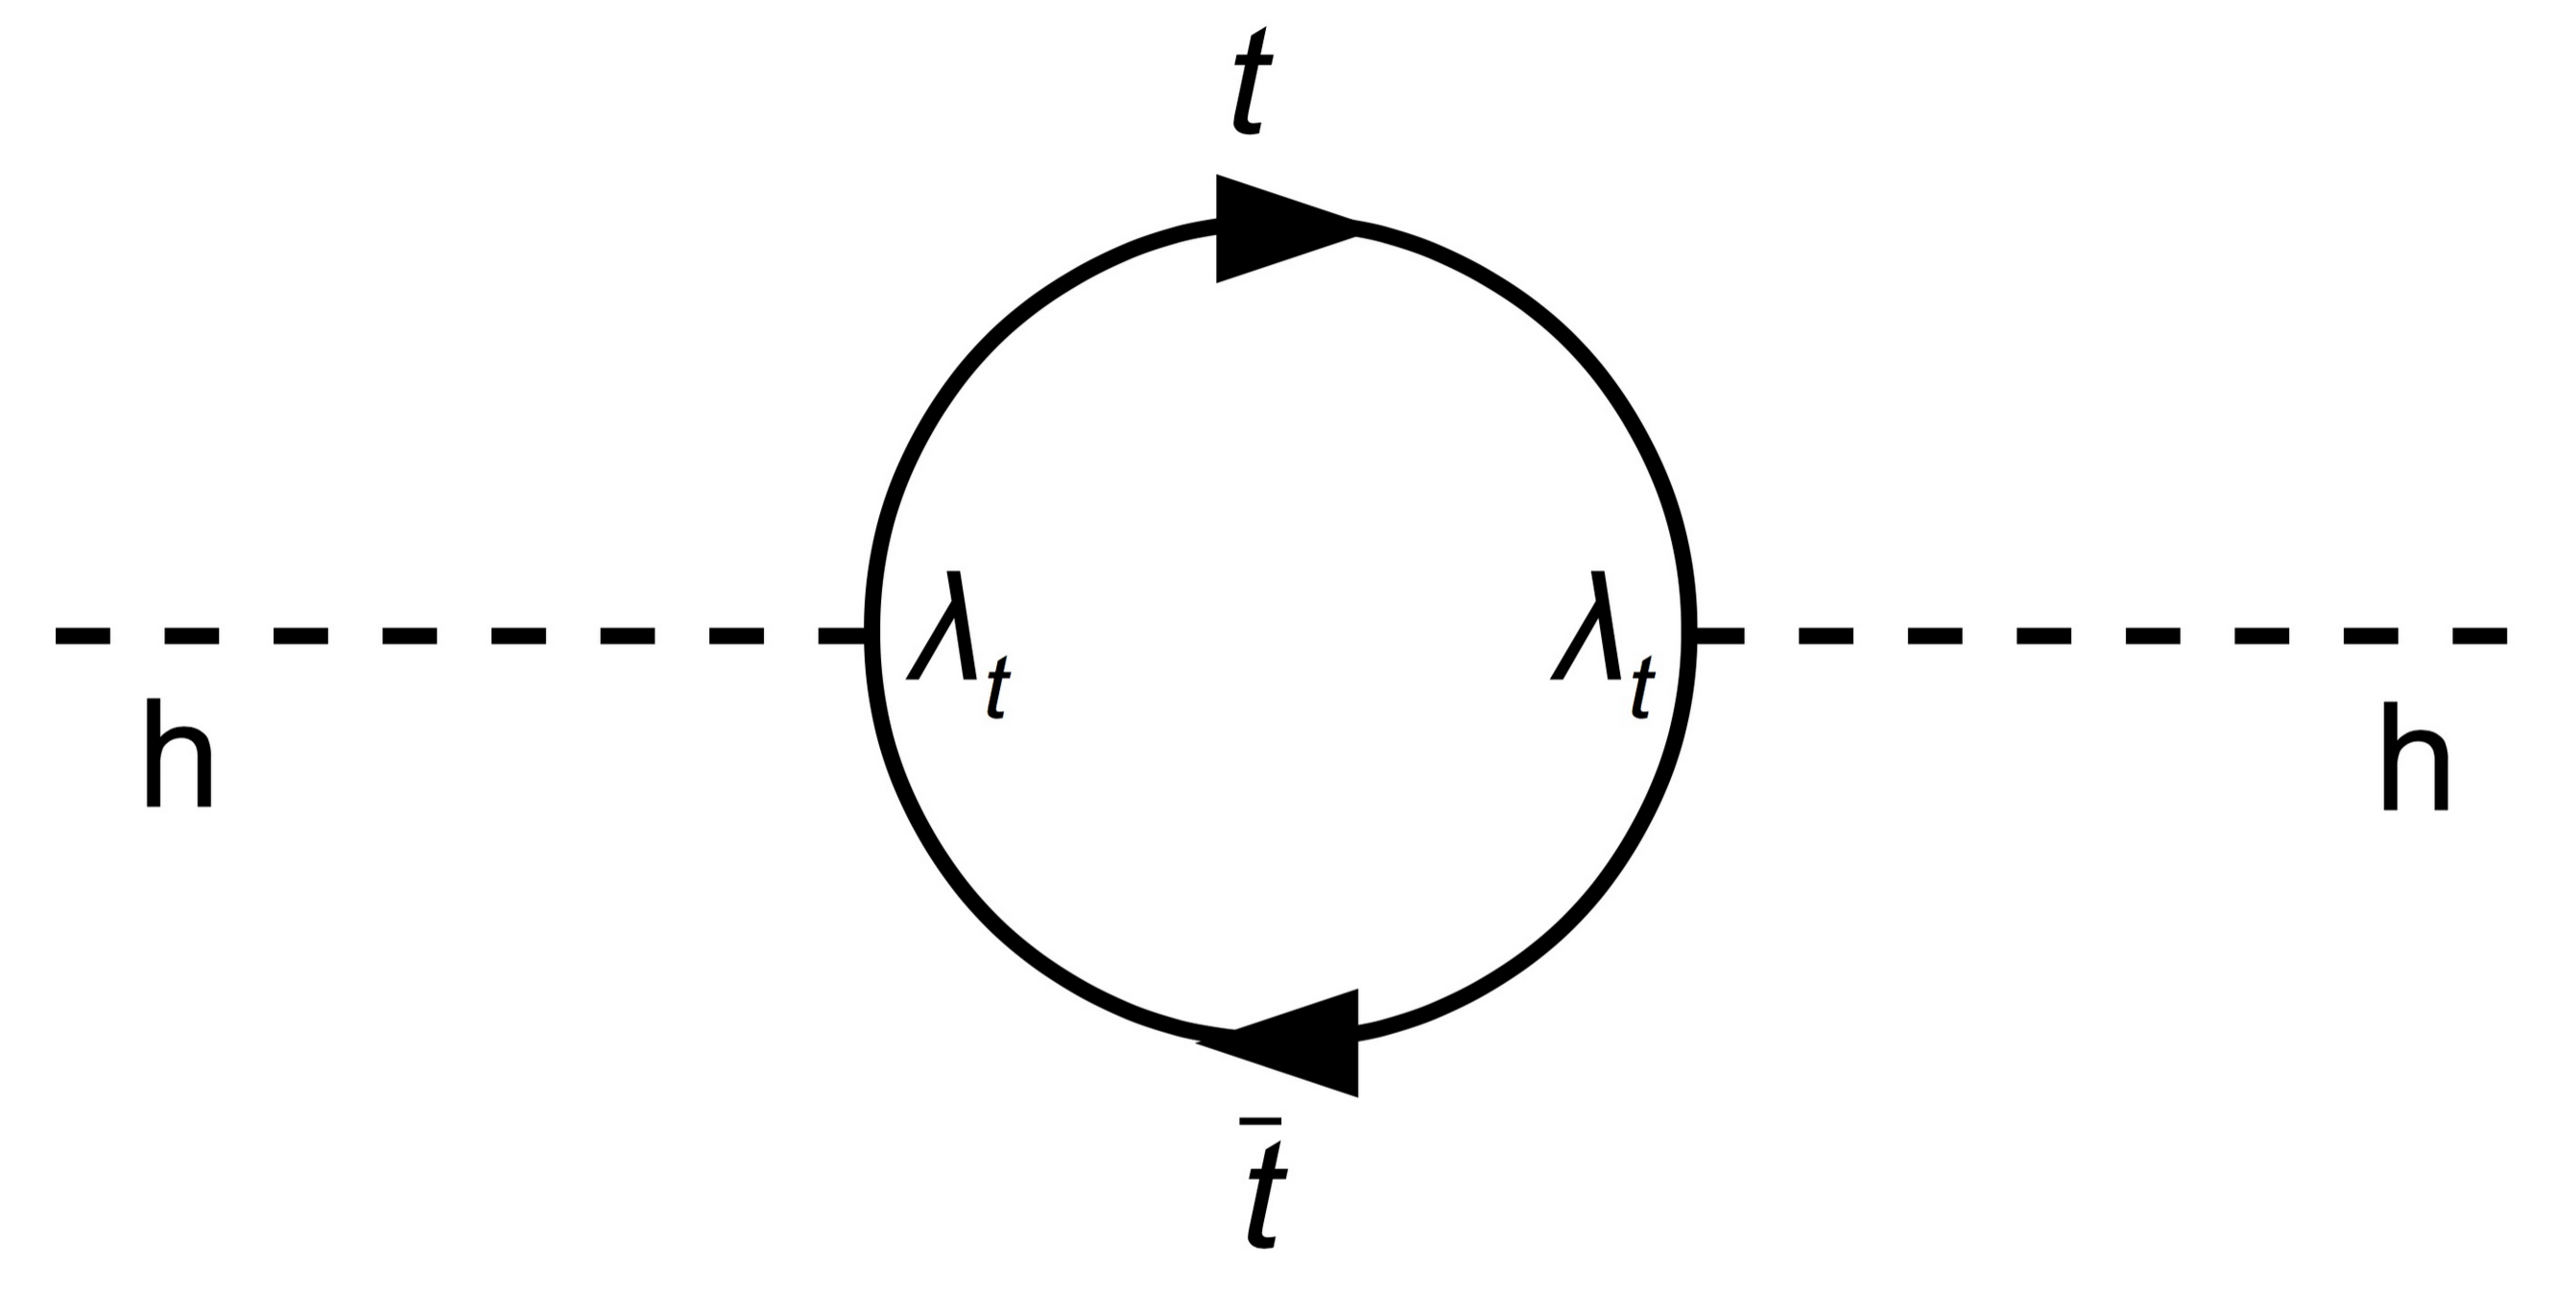
\includegraphics[width=0.35\textwidth]{top_loop}
    \caption[]{Leading correction to the Higgs field from top pair interaction. cite(https://onlinelibrary.wiley.com/doi/pdf/10.1155/2011/968283)}
    \label{fig:top_loop}
\end{figure}


A phase transition via quantum tunneling into a different \ac{vev} could result in the universe's particles, forces and structures ceasing to exist and being replaced by different ones. The stability of the universe, under the assumptions of \ac{sm} physics, critically depends on the precise values of the Higgs and top quark masses, as depicted in the phase diagram in figure \ref{fig:vev_stability}, which places the universe at the boundary between stability and metastability given current measurement accuracies.


\begin{figure}
    \centering
    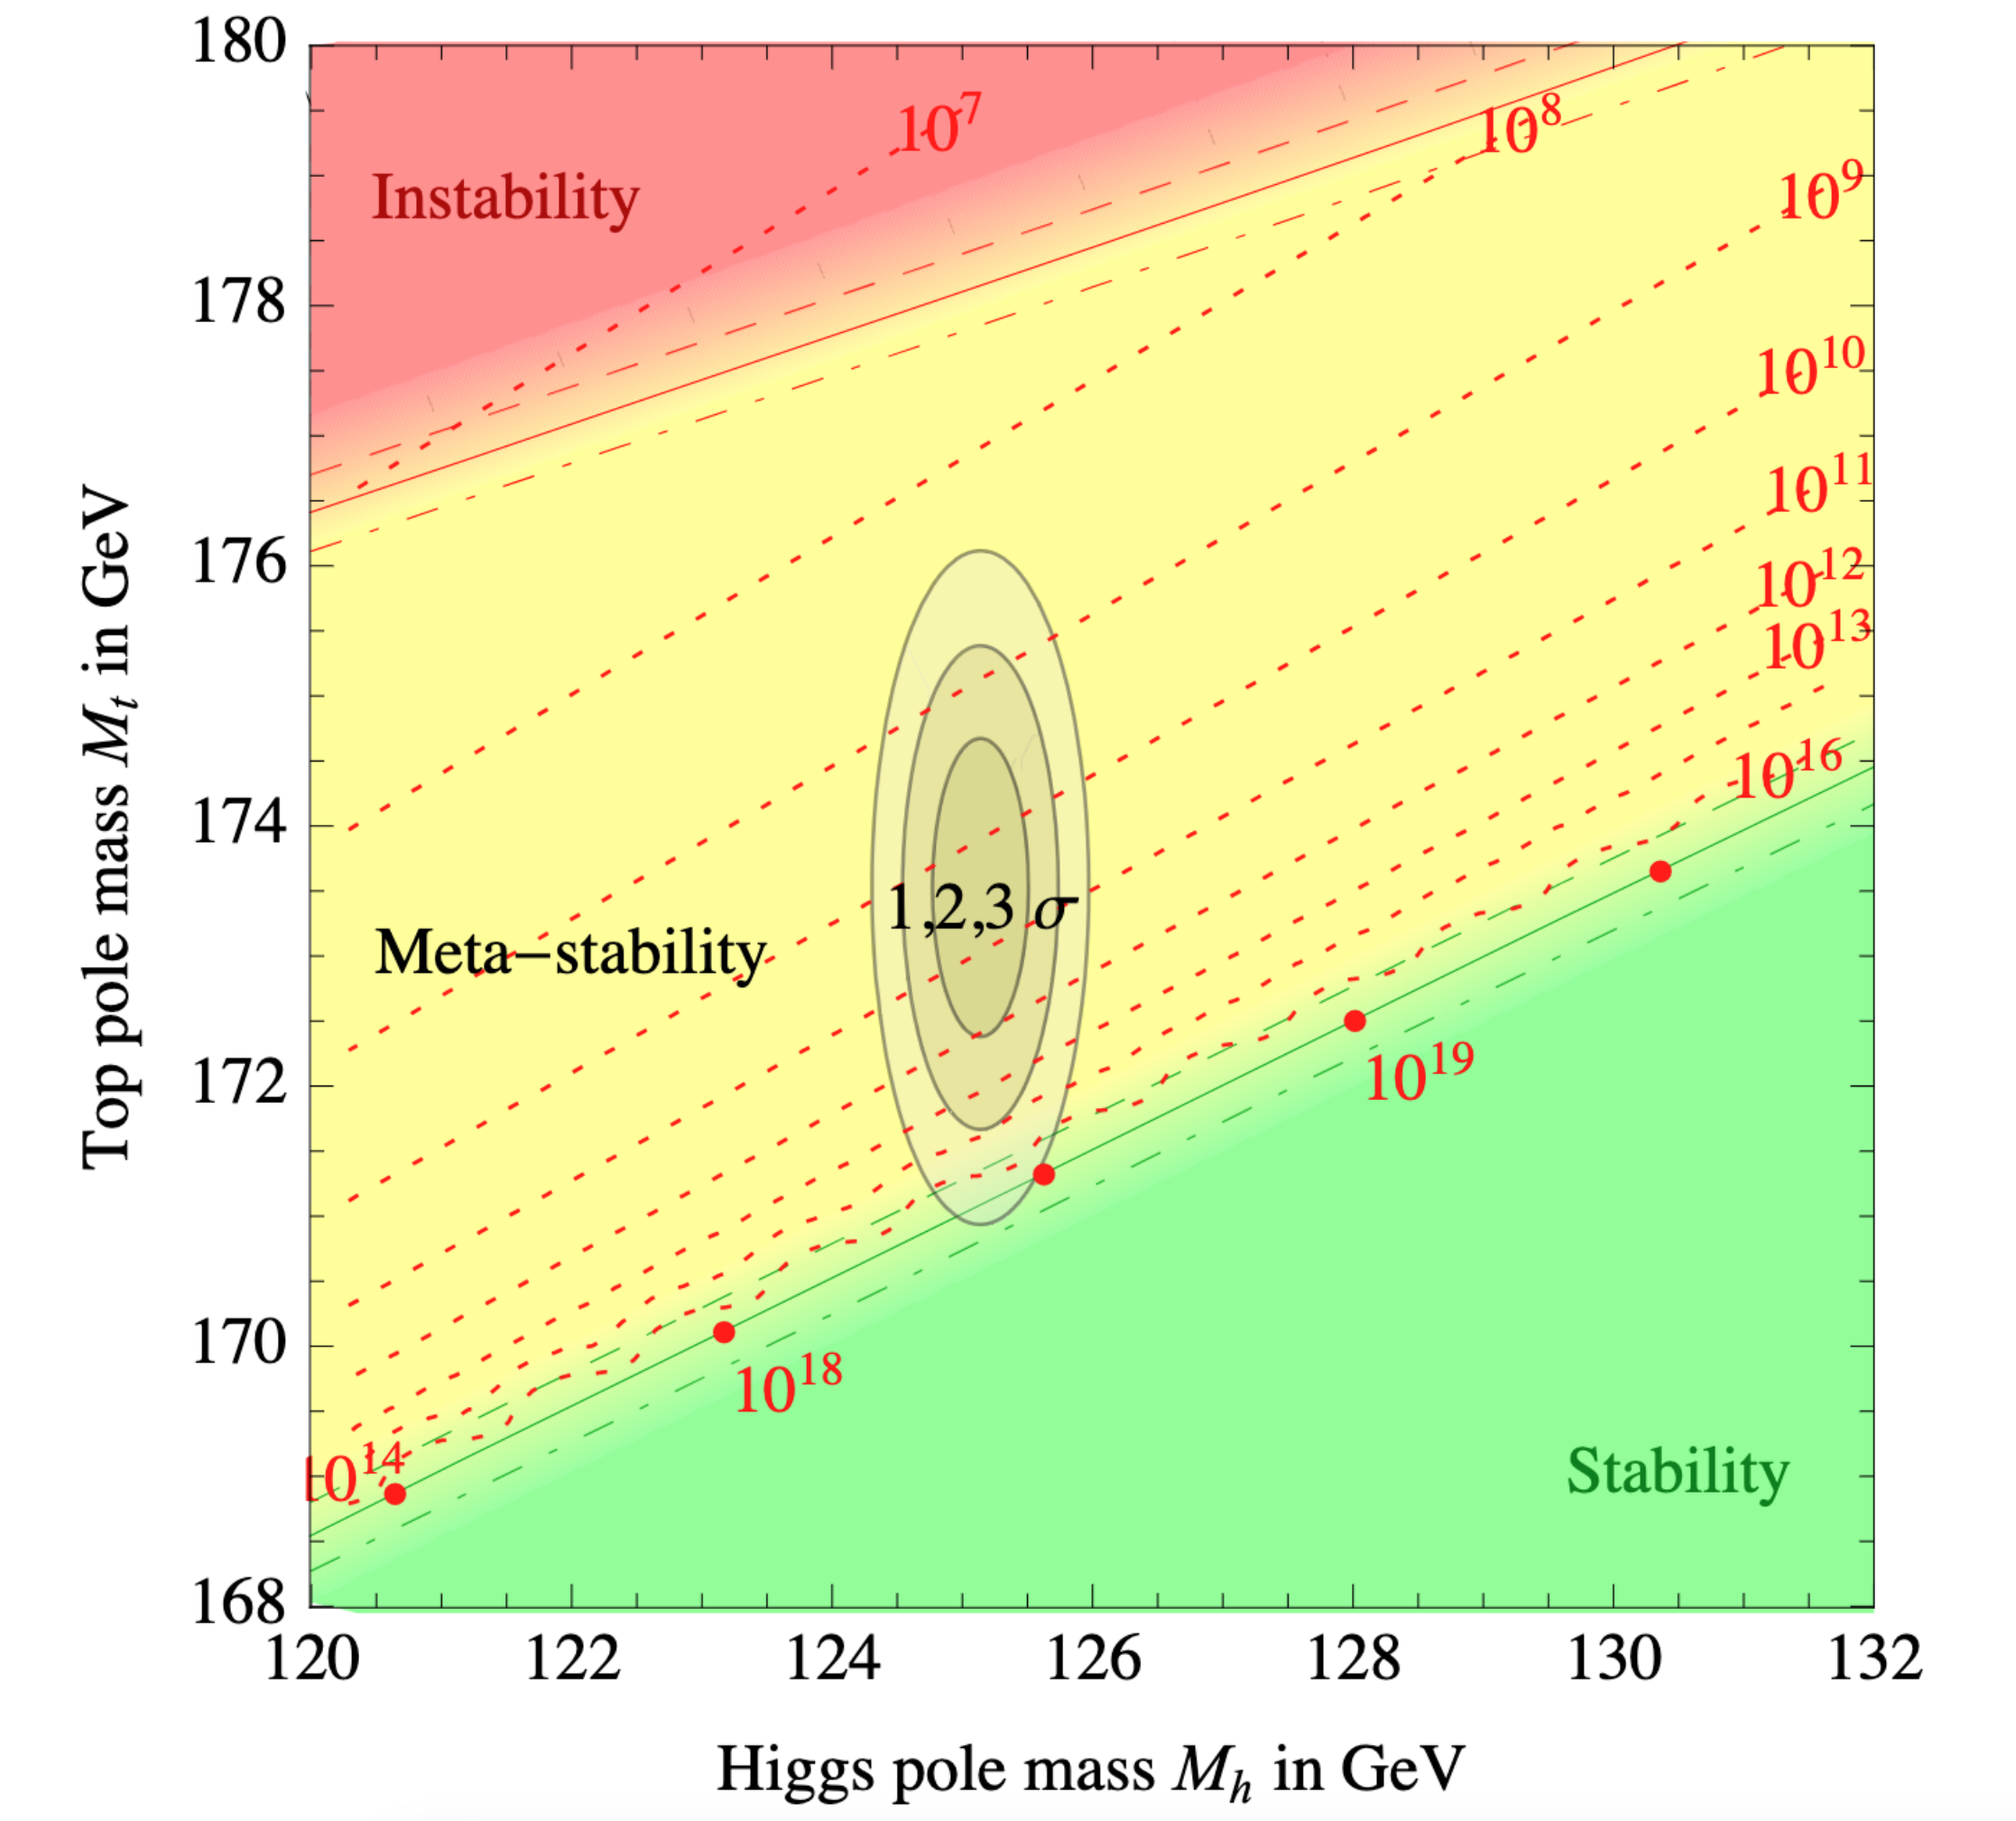
\includegraphics[width=0.7\textwidth]{vev_stability}
    \caption[]{Phase diagram of the stability of the universe assuming the \ac{sm} as a function of the Higgs and top pole masses. Instability for the Higgs potential occurs when due to quantum loop corrections the Higgs field develops a different minimum. Meta-stability is the case when there is an even lower global minimum in the potential and Stability means that there is only one global minimum. The red isolines correspond to the energy scale $\Lambda_I$ at which the Higgs potential becomes unstable. Adopted from \citep{Buttazzo:2013uya}.}
    \label{fig:vev_stability}
\end{figure}





Through the Higgs mechanism, elementary particles gain mass by interacting with the Higgs field. Accurate measurements of properties such as the mass and decay channels of the Higgs boson and the top quark offer means to validate and challenge the \ac{sm}. A precise understanding of these is crucial as any deviation from the expected values could indicate new physics. Moreover, the stability of our universe might be related to these properties. The study of the Higgs potential is therefore a promising endeavor to which this work aims to contribute.


\chapter{The ATLAS experiment at the Large Hadron Collider}\label{sec:atlas}
Exploring the nature of the Higgs particle requires collision energies on the \qty[]{}{TeV} scale. The \ac{lhc} is currently the most powerful particle accelerator making it the best available facility for studying the Higgs particle. The main reference for this section is \citep{aad2008atlas}.

\section{The Large Hadron Collider}
The \ac{lhc} is a circular proton proton collider with \qty[]{27}{km} circumference with a center-of-mass energy of $\sqrt{s}=\qty[]{13}{TeV}$. The two anticyclic proton beams are actually bunches containing $10^{11}$ protons that are brought to collisions at several points of the ring for the experiments performed at the \ac{lhc}. A measure of how tightly particles are packed in these bunches is the instantaneous luminosity and is characteristic to the collider
\begin{equation}
    L=\frac{1}{\sigma}\frac{\dint{N}}{\dint{t}}.
\end{equation}
It can be read as particle interactions per unit time and area. The area understood as the interaction cross-section of a particular process. The total recorded number of collision events can thus be calculated by summing the luminosity over time which gives with the integrated luminosity
\begin{equation}
    N=\sigma\cdot\int L dt=\sigma\cdot L_\mathrm{int}.
\end{equation}
For the full run 2 dataset used in this thesis the integrated luminosity for events good for physics analysis is \qty[]{140.1}{fb^{-1}} \citep{DAPR-2021-01}.

\section{The ATLAS detector}
The \ac{atlas} (A Toroidal LHC Apparatus) experiment is a particle detector with an onion-like structure, as shown in figure \ref{fig:atlas_detector}.
\begin{figure}
    \centering
    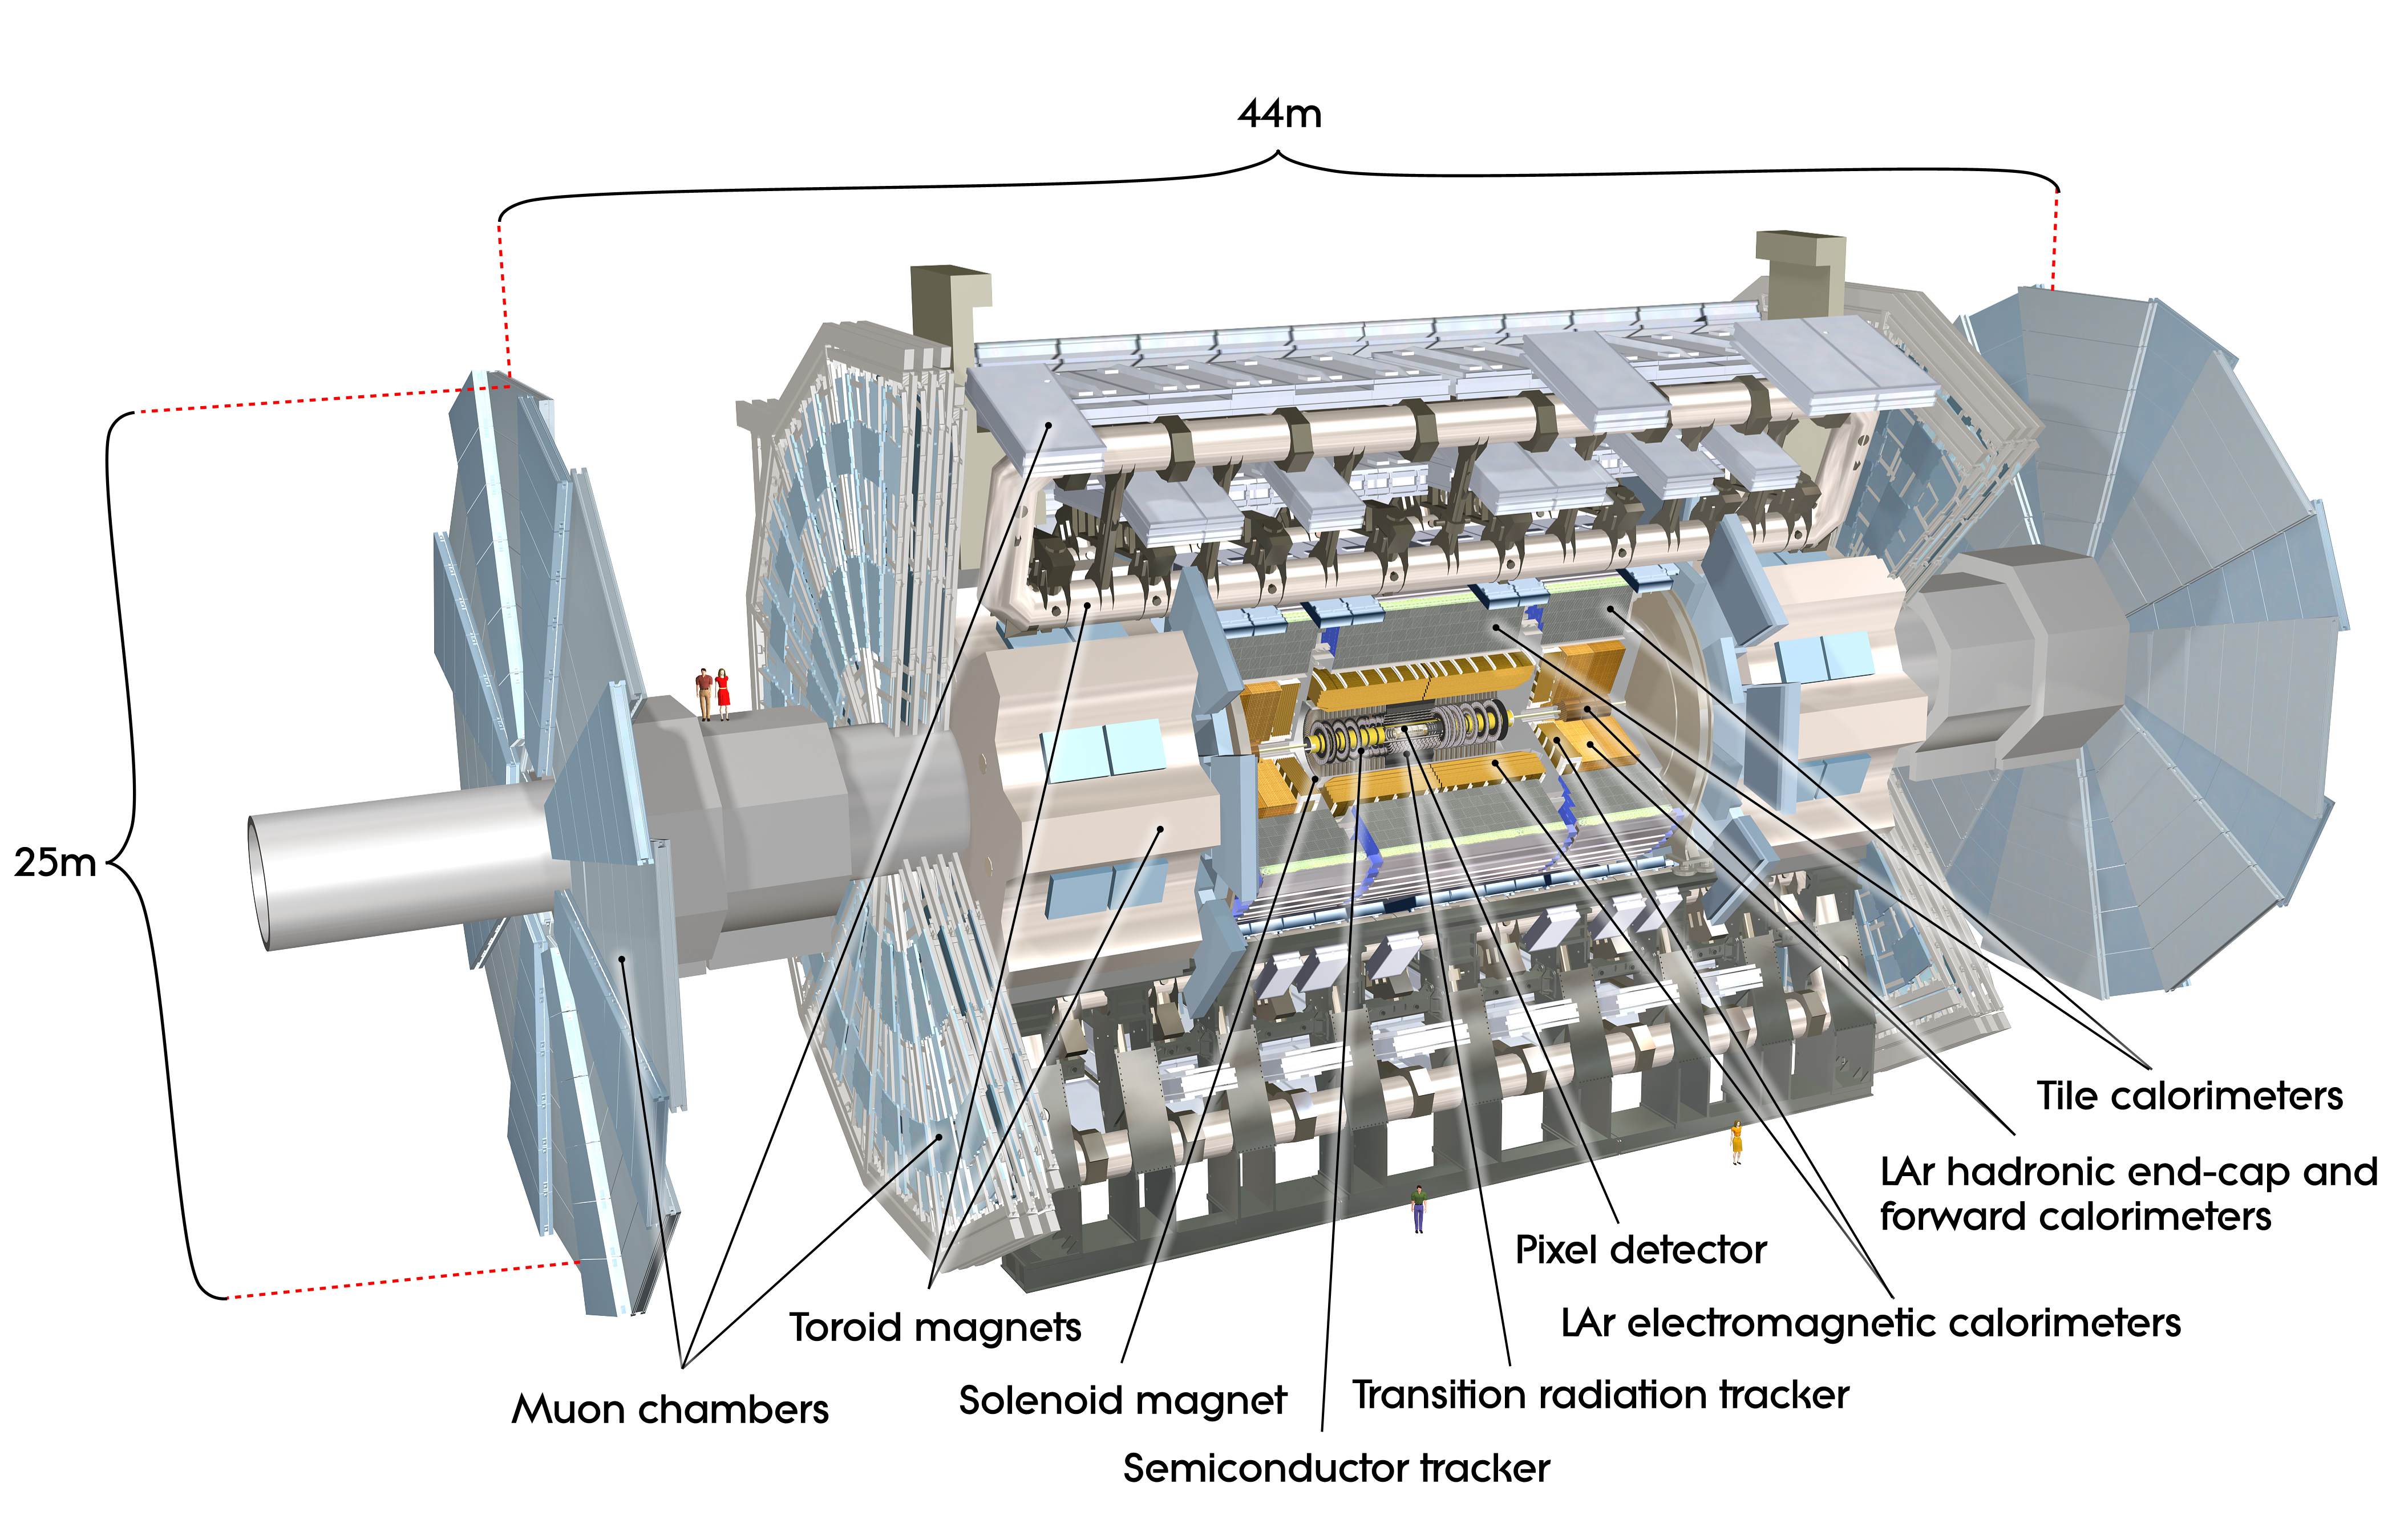
\includegraphics[width=1\textwidth]{atlas_detector}
    \caption[]{The \ac{atlas} experiment at the \ac{lhc} with its subdetectors. Adopted from \citep{Pequenao:1095924}.}
    \label{fig:atlas_detector}
\end{figure}
Its purpose is to measure the trajectory, momentum, and energy of particles originating from proton-proton collisions, depending on the particular kind of interaction of the collision products with matter. The various subdetectors are explained below from the inside out.

\subsection*{Coordinate System}
The coordinate system of \ac{atlas} is right-handed and originates at the interaction point at the center of the detector. The z-axis points along the beam line, the x-axis to the center of the lhc and the y-axis away from earth. Thus quantities transversal to the z-axis are Lorentz-invariant. Inside the detector cylindrical coordinates $r,\phi$ are used with $\phi$ the azimuthal angle about the z-axis and the polar angle $\Theta$ of a particle measured in form of the pseudorapidity $\eta=-\ln(\Theta/2)$. This quantity is defined as an approximation for the Lorentz invariant rapidity and holds for highly relativistic particles. With these a useful quantity to describe angular distances in the detector is
\begin{equation}
    \Delta R = \sqrt{(\Delta\phi)^2+(\Delta \eta)^2}.
    \label{eq:delta_R}
\end{equation}

\section{Inner detector}\label{sec:inner_detector}
The inner detector, shown schematically in figure \ref{fig:inner_tracker}, is designed to track charged particles and figure out their momentum and provide information on the particle type.
\begin{figure}
    \centering
    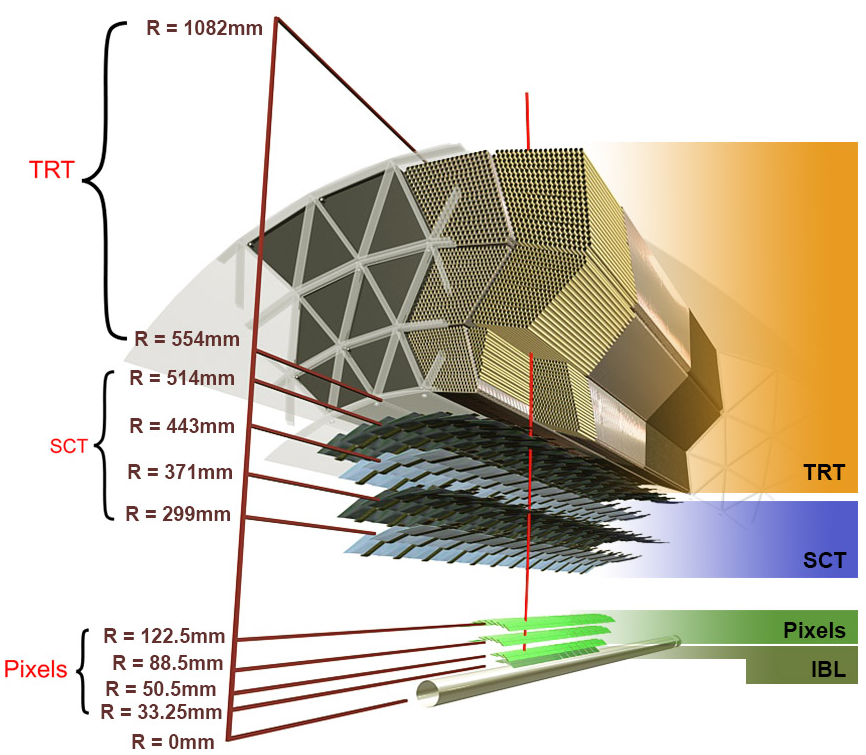
\includegraphics[width=0.65\textwidth]{inner_tracker}
    \caption[]{The inner detector schematically with the subdetectors described in the full text. Adopted from \citep{Potamianos:2016ptf}.}
    \label{fig:inner_tracker}
\end{figure}
It is surrounded by a solenoid magnet whose field lines point in the direction the beam so that charged particles are bent in the transverse plane of the detector due to the Lorentz force. The bending direction reveals the charge whereas the curvature depends on the momentum.

The \ac{ibl}, pixel detector, and \ac{sct} all consist of silicon detectors of various sizes. When passing through silicon, charged particles ionize electrons that travel in an electric field to an electrode and provide positional information. The \ac{ibl} plays a crucial role in b-tagging as will become clear in section \ref{sec:b_tagging}.

Aforementioned semiconductor trackers are surrounded by the \ac{trt} which apart from tracking also can identify particles. It consists of several layers of tubes perpendicular to the beamline, filled with a gas mixture, and a conducting wire in their center, which is under voltage and attracts negative charges. The tubes are surrounded in a material with different permittivity so that charged particles passing through the boundaries of the material emit transition radiation. The intensity of this radiation depends on the velocity, so that for particles of the same energy more photons are released for the lighter particle. Therefore for electrons for example can be distinguished from pions.

\section{Calorimeters}

When high-energy particles pass through dense matter the various particle interactions create secondary particles that result in a particle shower. Via this the energy of particles can be inferred and is done in \ac{atlas} with two sampling calorimeters. These consist of alternating layers of a high-density metal to absorb the energy and a material that can track the particles of the shower.

\subsection*{Electromagnetic Calorimeter}

In the electromagnetic calorimeter the main energy deposits are from electrons and photons. The stopping material consists of lead and steel and is alternated with a copper plate on which there is an electrode grid. Between the plates is liquid argon. When interacting with the dense metal e.g. by bremsstrahlung of an electron or by pair production induced by a photon, the created secondary particles ionize the argon atoms in between. The negatively charged ions are then pulled to the charged copper electrodes to determine the position. From the distance a particle has traveled through the electromagnetic calorimeter, one can infer the energy of the particle as it entered the calorimeter.

\subsection*{Hadronic Calorimeter}

Hadrons also deposit energy in the electromagnetic calorimeter but interact with nuclei as well. However as they are more energetic more stopping power is needed which is provided by the hadronic calorimeter that surrounds the electromagnetic calorimeter. The configuration is made of many layers of tiles positioned in planes perpendicular to the beamline. In these layers tiles of steel as stopping material alternate by a scintillating plastic which radiates light if charged particles pass through. The light is collected at the edges by wavelength-shifting optical fibres  which reduce the energy of the photons and then read out by photomultiplier tubes.

\section{Muon Spectrometer}

The muon spectrometer encircles all other detectors to capture muons which barely loose energy passing through the other detectors. Its basic units are resistive plate chambers in three layers around the calorimeters. These are basically large charged capacitors filled with gas. When charged particles pass through they ionize the gas and the resulting avalanche of ions drawn to the electrodes is measured to determine the position and time of flight through the plates.  In addition, they are also used in a design where the electrodes consist of a tube filled with gas and a wire inside similar to the \ac{trt}. The entire spectrometer is placed in a toroidal magnetic field so that the field lines are in phi direction in order to also measure the momentum due to the curvature of the muons.

The figure \ref{fig:particles_in_detector} shows where which type of particles are stopped in the different detectors.
\begin{figure}
    \centering
    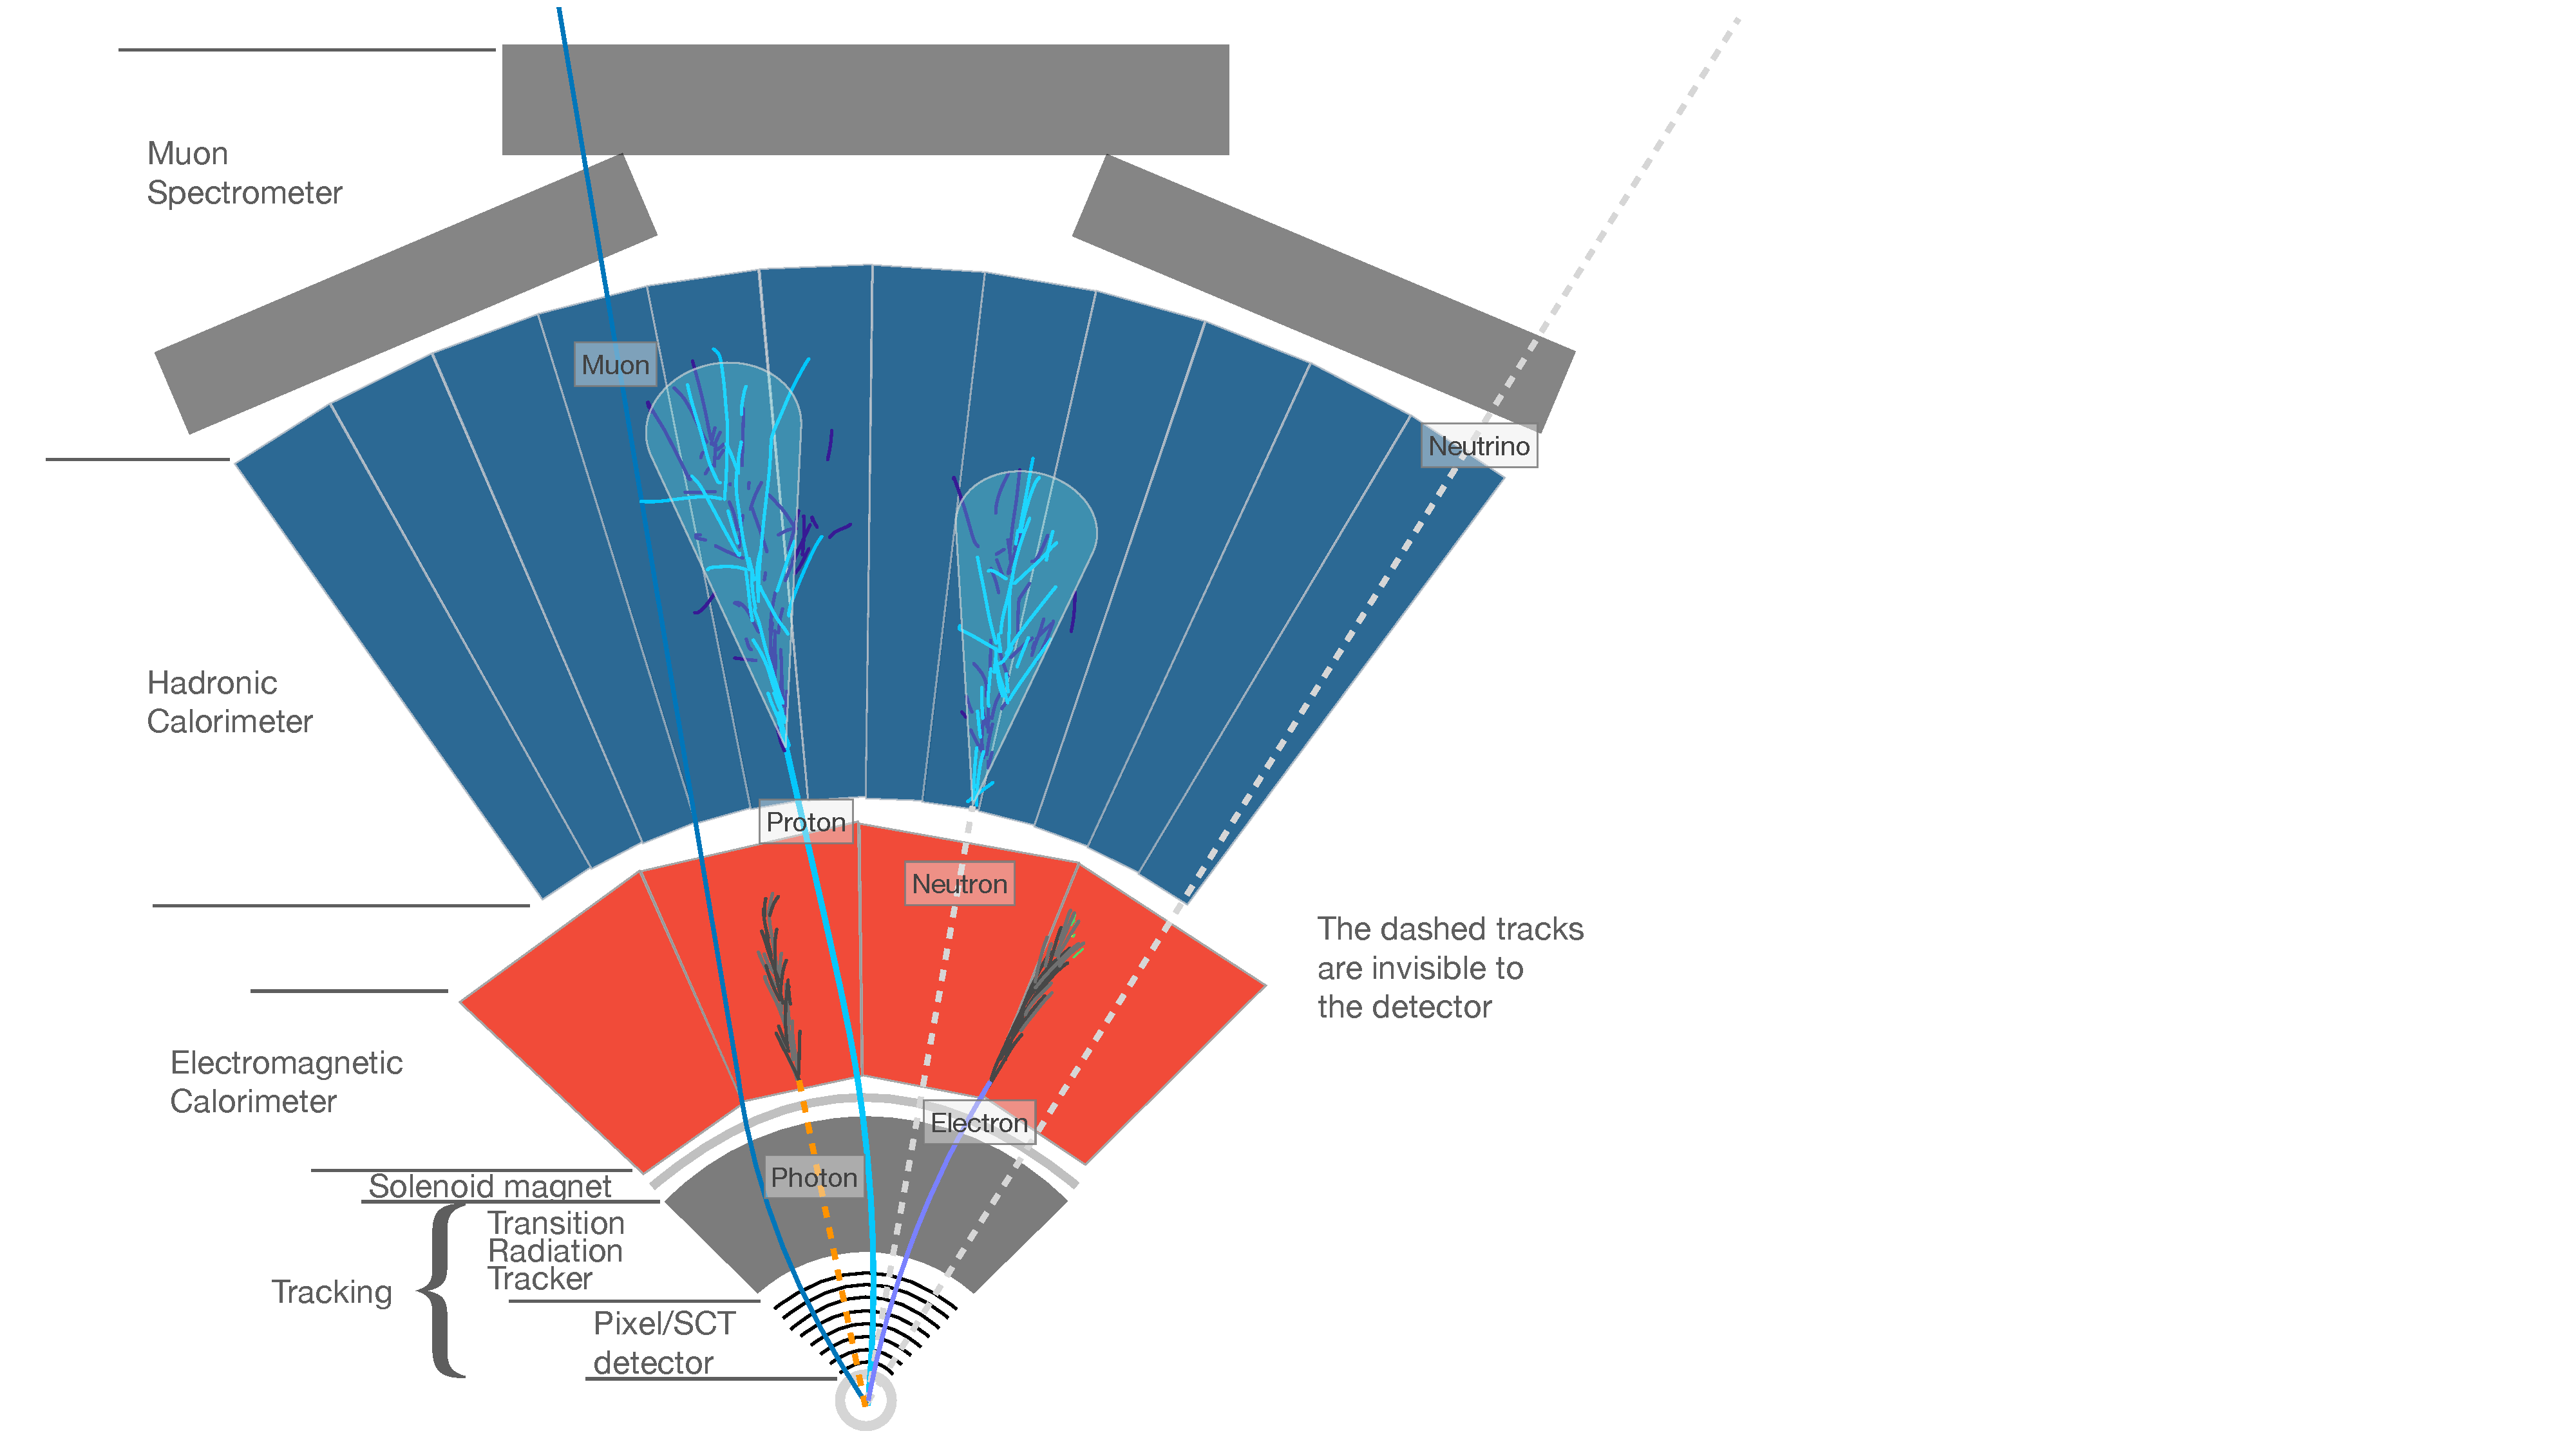
\includegraphics[width=1\textwidth]{particle-shower}
    \caption[]{Paths and energy deposits of particle types in the subdetectors. Adopted from \citep{Guth:2765038}.}
    \label{fig:particles_in_detector}
\end{figure}

\section{Data Acquisition}\label{sec:tdaq}
Bunches of protons in the \ac{lhc} are brought to collision in \ac{atlas} with a rate of \qty[]{40}{MHz}. It is technically impossible at the moment to record all collisions as this would correspond to a data rate of \qty[]{40}{TB\per s}. Therefore events that are useful for physics analysis need to be preselected which is called triggering and is performed in two steps. The first step is the \ac{l1} trigger and is hardware based and reduces the event rate to \qty[]{100}{kHZ}. This is done by selecting events with large transverse momentum deposits in the detector and also for events with missing transverse momentum. Afterwards the regions in the detector where this is the case are passed to a software \ac{hlt}. This then uses the full detector information in these regions to reduce the rate further down to \qty[]{1}{kHz}.

% \section{Statistics}\label{sec:statistics}

Every scientific investigation starts with a hypothesis that is to be tested empirically. The main objective is to evaluate if the proposed hypothesis agrees or disagrees with observed data, to either accept or reject it against the null-hypothesis. The metric at hand to do so is the p-value that arises within hypothesis testing. 

In the field of high energy physics, a framework based on likelihood statistics has been developed specifically for this task. This section begins to lay out the mathematical fundamentals of the approach and explains its implementation in \textsc{pyhf} \citep{pyhf,pyhf_joss}. The following is based on \citep{cowan2011asymptotic,behnke2013data,pyhf}.
 
\subsection{Building the likelihood}\label{sec:likelihood}
The statistical model must take into account how compatible are the theoretical predictions with the observed collision events. This can be described by a likelihood $L(\bm{x} | \bm{\phi})$ which is in in general a probability for an observation $\bm{x}$ under a given set of parameters $\bm{\phi}$. Through $\bm{\phi}$ the theoretical predictions are incorporated into the probability calculation. Given that this is a counting experiment, the preferred tool of analysis are bins of a histogram $\bm{h}=(h_1,...,h_N)$.

It is useful to subdivide a measurement $\bm{x}=(\bm{n},\bm{a})$ further into observable histograms $\bm{n}$, (e.g. the invariant mass of a particle) and auxiliary measurement histograms $\bm{a}$ that help to constrain the model. Additionally, in the context of hypothesis testing it is useful to split the set of parameters $\bm{\phi}=(\bm{\psi},\bm{\Theta})$ into so-called parameters of interest $\bm{\psi}$ and nuisance parameters $\bm{\Theta}$. For this subsection it is instructive to consider only one parameter of interest, the signal strength $\mu$. 

The bin contents can then be expressed in terms of the amount of signal $s_i(\bm{\Theta})$ and background $b_i(\bm{\Theta})$ in bin $i$ that depend on the nuisance parameters. The prediction (expectation value) of the histogram bins of the observable $n_i$ can then be expressed as 
\begin{equation} \label{eq:n_i}
    \langle n_i(\mu,\bm{\Theta})\rangle = \mu s_i(\bm{\Theta}) +b_i(\bm{\Theta}). 
\end{equation}
Similarly, for auxiliary measurement bins $a_i$ their expectation value can be calculated from functions $u_i(\bm{\Theta})$ that also depend on the nuisance parameters and help to constrain the model
\begin{equation} \label{eq:a_i}
    \langle a_i(\bm{\Theta}) \rangle = u_i(\bm{\Theta}).
\end{equation}
Since this is a counting experiment in which events occur at a constant mean rate and independently of time, each bin follows a Poisson distribution
\begin{equation}\label{eq:poisson}
    \frac{r^k e^{-r}}{k!}.
\end{equation}
$r$ is the expected rate of occurrences, which translates as our prediction, whereas $k$ are the actual measured occurrences. Therefore the likelihood is a product of Poisson probabilities
\begin{equation}\label{eq:likelihood}
    L(\mu,\bm{\Theta})=
    \prod_{j=1}^N \frac{(\mu s_j(\bm{\Theta}) + b_j(\bm{\Theta}))^{n_j}}{n_j !} e^{-(\mu s_j(\bm{\Theta}) + b_j(\bm{\Theta}))}
    \prod_{k=1}^M \frac{u_k(\bm{\Theta})^{a_k}}{a_k!} e^{-u_k(\bm{\Theta})}.
\end{equation}
The last product can also be thought of penalizing the likelihood if e.g. an auxiliary measurement displays a very improbable value for a quantity. To test for a hypothesized value of $\mu$, the best choice according to the Neyman-Pearson lemma \citep{behnke2013data}, is the profile likelihood ratio that reduces the dependence to the parameter(s) of interest
\begin{equation}\label{eq:likelihood_ratio}
\lambda(\mu)=
    \frac{L(\mu,\hat{\hat{\bm{\Theta}}})}
    {L(\hat{\mu},\hat{\bm{\Theta}})}.
\end{equation}
The denominator is the unconditional maximum likelihood estimation so that $\hat{\mu}$ and $\hat{\bm{\Theta}}$ both are free to vary to maximize $L$, whereas the numerator is the found maximum likelihood conditioned on some chosen $\mu$ and the set of nuisance parameters $\hat{\hat{\bm{\Theta}}}$ that maximize the likelihood for that particular $\mu$. This definition gives $0 \leq \lambda \leq 1$. For a $\lambda \approx 1$ the hypothesized value of $\mu$ shows good agreement to the Poissonian model.

\subsection{From test statistic to p-value}
For this subsection $\mu$ can be a set of parameters of interest (defined above as $\bm{\psi}$) to be consistent with the usage in the literature. To test for alternative hypotheses it is useful to transform the profile likelihood into a test statistic $t_{\mu}$ 
\begin{equation}
    t_{\mu}=-2\log \lambda(\mu).
\end{equation}
This translates to $t_{\mu} \rightarrow 0$ as good agreement and $t_{\mu} \rightarrow \infty$ as bad agreement to the model. A right-tail p-value can then be calculated from the probability density function of $t_\mu$: \acp{pdf}$(t_\mu) = f(t_\mu \mid \mu)$
\begin{equation}\label{eq:p-value}
    p_\mu = \int_{t_{\mu ,obs}}^{\infty} 
    f(t_\mu \mid \mu) \mathrm{d}t_\mu
\end{equation}
$t_{\mu ,obs}$ is the test statistic $t_\mu$ evaluated with the observed data. This is like finding the $\mu$ for which the likelihood in the numerator of the profile likelihood ratio in equation \ref{eq:likelihood_ratio} would have the same prediction as the observation ($\mu s_j(\hat{\hat{\bm{\Theta}}}) + b_j(\hat{\hat{\bm{\Theta}}})\stackrel{!}{=}n_j$ in the likelihood of equation \ref{eq:likelihood}). Just like a probability density function for a standard normal distribution, intuitively the \acp{pdf} is how probable a particular value of the test statistic $t_\mu$ is under a fixed value of the signal strength (how often it occurs compared to all other values $t_\mu$ can have). 

This particular form is handy because there exist approximations for $f(t_\mu \mid \mu)$ \citep{cowan2011asymptotic}. Wald \citep{wald1943tests} proved that for the null hypothesis in the large sample limit, the test statistic follows a normalized sum of squared distances between the tested parameters of interest $\mu$ and its maximum likelihood estimate $\hat{\mu}$. The result was extended by Wilk \citep{wilks1938large} for any hypothesis, so the test statistic becomes
\begin{equation}
    t_\mu=\sum_i \frac{(\mu_i-\hat{\mu}_i^2)}{\sigma_i^2} + \mathcal{O}(1/\sqrt{N}).
\end{equation}
The $\hat{\mu}_i$ are in the large sample limit normally distributed with mean $\mu'$ (true values) and standard deviation $\sigma_i$. This is the definition of a non-central $\chi$-squared distribution with degrees of freedom equal to the number of parameters of interest (see section 3.1 in \citep{cowan2011asymptotic}). For one parameter of interest the distribution reads
\begin{equation}\label{eq:chi-square}
    f(t_\mu \mid \mu)=\frac{1}{2\sqrt{t_\mu}}\frac{1}{\sqrt{2\pi}}
    \left[
\exp\left(-\frac{1}{2}\left(\sqrt{t_\mu}+\sqrt{\Lambda}_\mu\right)\right)
+
\exp\left(-\frac{1}{2}\left(\sqrt{t_\mu}-\sqrt{\Lambda}_\mu\right)\right)
\right],
\end{equation}
with non-centrality parameter 
\begin{equation}
    \Lambda_\mu=\frac{(\mu-\mu')^2}{\sigma^2}.
\end{equation}
Figure \ref{fig:test_stat_example} illustrates the different steps. Being able to calculate p-values allows now to state how likely it is that the proposed hypothesis is reflected by the observed data. In other words, the p-value represents the probability, how incompatible the proposed hypothesis (prediction) is with the observation.

In the scientific community a widely accepted threshold for this is a p-value of 0.05. Though particle physicists only claim discovery of a new phenomenon for $p$ < \qty{2.87e-7}{} corresponding to 5 standard deviations of the standard normal distribution and exclude hypotheses if the p-value is not below 2 standard deviations of the standard normal distribution $p$ $\lesssim$ \qty{0.05}{}. One caveat here is that this particular form of $t_\mu$ assumes $\mu$ can also be negative, which can be non-physical depending on the impact of a new process. Test statistics and their \acp{pdf} approximations considering the different cases are covered in \citep{cowan2011asymptotic}. 
\begin{figure}
    \centering
    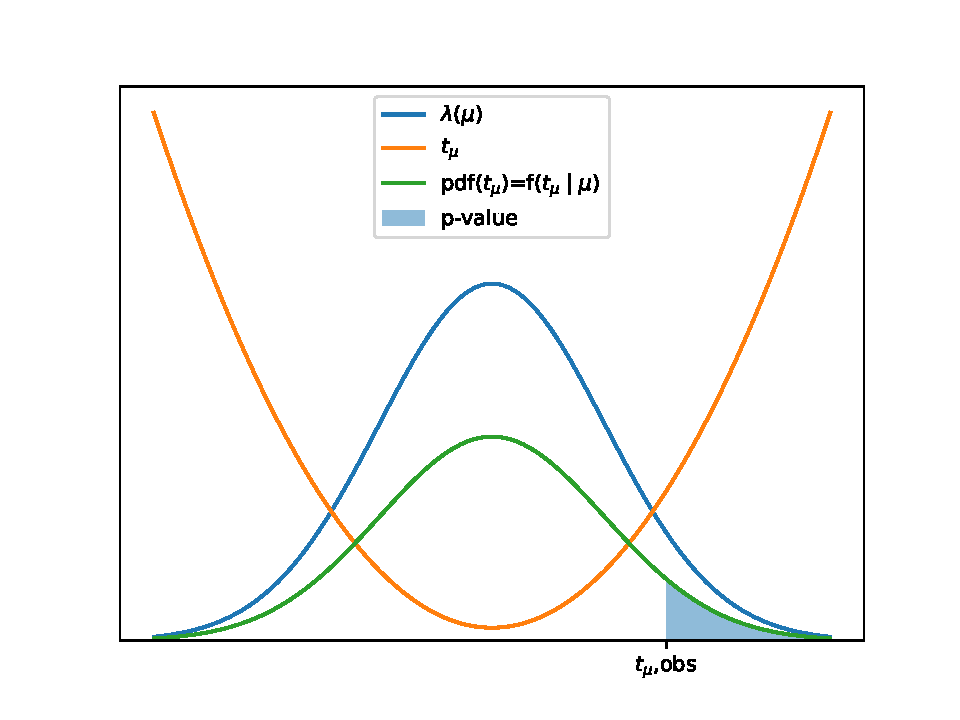
\includegraphics[width=0.8\textwidth]{test_stat_example.pdf}
        \caption[]{A sketch to follow the steps to calculate p-values. (\textbf{left}) The profile likelihood (\hexbox{1f77b4}) has essentially some hill-like form with a maximum at ${\lambda(\hat{\mu},\hat{\bm{\Theta}})}$, $t_\mu$ (\hexbox{ff7f0e}) is $-2\mathrm{ln}(\lambda)$. (\textbf{right}) For one parameter of interest in the large sample limit $f(t_\mu \mid \mu)$ follows a non-central chi-squared distribution with one degree of freedom, equation \ref{eq:chi-square}. The blue shaded area under the \acp{pdf} is a right hand sided p-value.}
    \label{fig:test_stat_example}    
\end{figure}

\subsection{The CL$_s$ value}\label{sec:cls}

Particle physicists are usually interested in two things when making statistical tests for the discovery of new phenomena: how well is the modeling of backgrounds (things we know) and whether there is evidence in the observations for a new phenomenon. This means one needs to test two hypotheses: a background only ($b$) and a signal plus background ($s+b$) hypothesis. Each will result in a p-value of their own. For example, $p_{b}=0$ would mean that the backgrounds are perfectly reflected by the observations and a $p_{s+b} < 0.05$ could be a sign of e.g. new physics. To combine these two metrics into a single score, particle physicists came up with the pseudo Confidence Level/p-value called CL$_s$ incorporating also the goodness of the modeling of the backgrounds 
\begin{equation}
    \mathrm{CL}_s=\frac{p_{s+b}}{1-p_{b}}=
    \frac
    {\int_{t_{\mu ,obs}}^{\infty} 
    f(t_{\mu,\,s+b} \mid \mu) \mathrm{d}t_\mu}
    {1-\int_{t_{\mu ,obs}}^{\infty} 
    f(t_{\mu,\,b} \mid \mu) \mathrm{d}t_\mu}.
\end{equation}
Intuitively the numerator is again just the value for the alternative hypothesis whereas the denominator penalizes CL$_s$ if the modeling of the backgrounds is not reflected in the observations. This can also be understood visually from the first figure of the paper that introduced the CL$_s$ quantity \citep{read2002presentation} (see description of fig. \ref{fig:cls}).
\begin{figure}
    \centering
    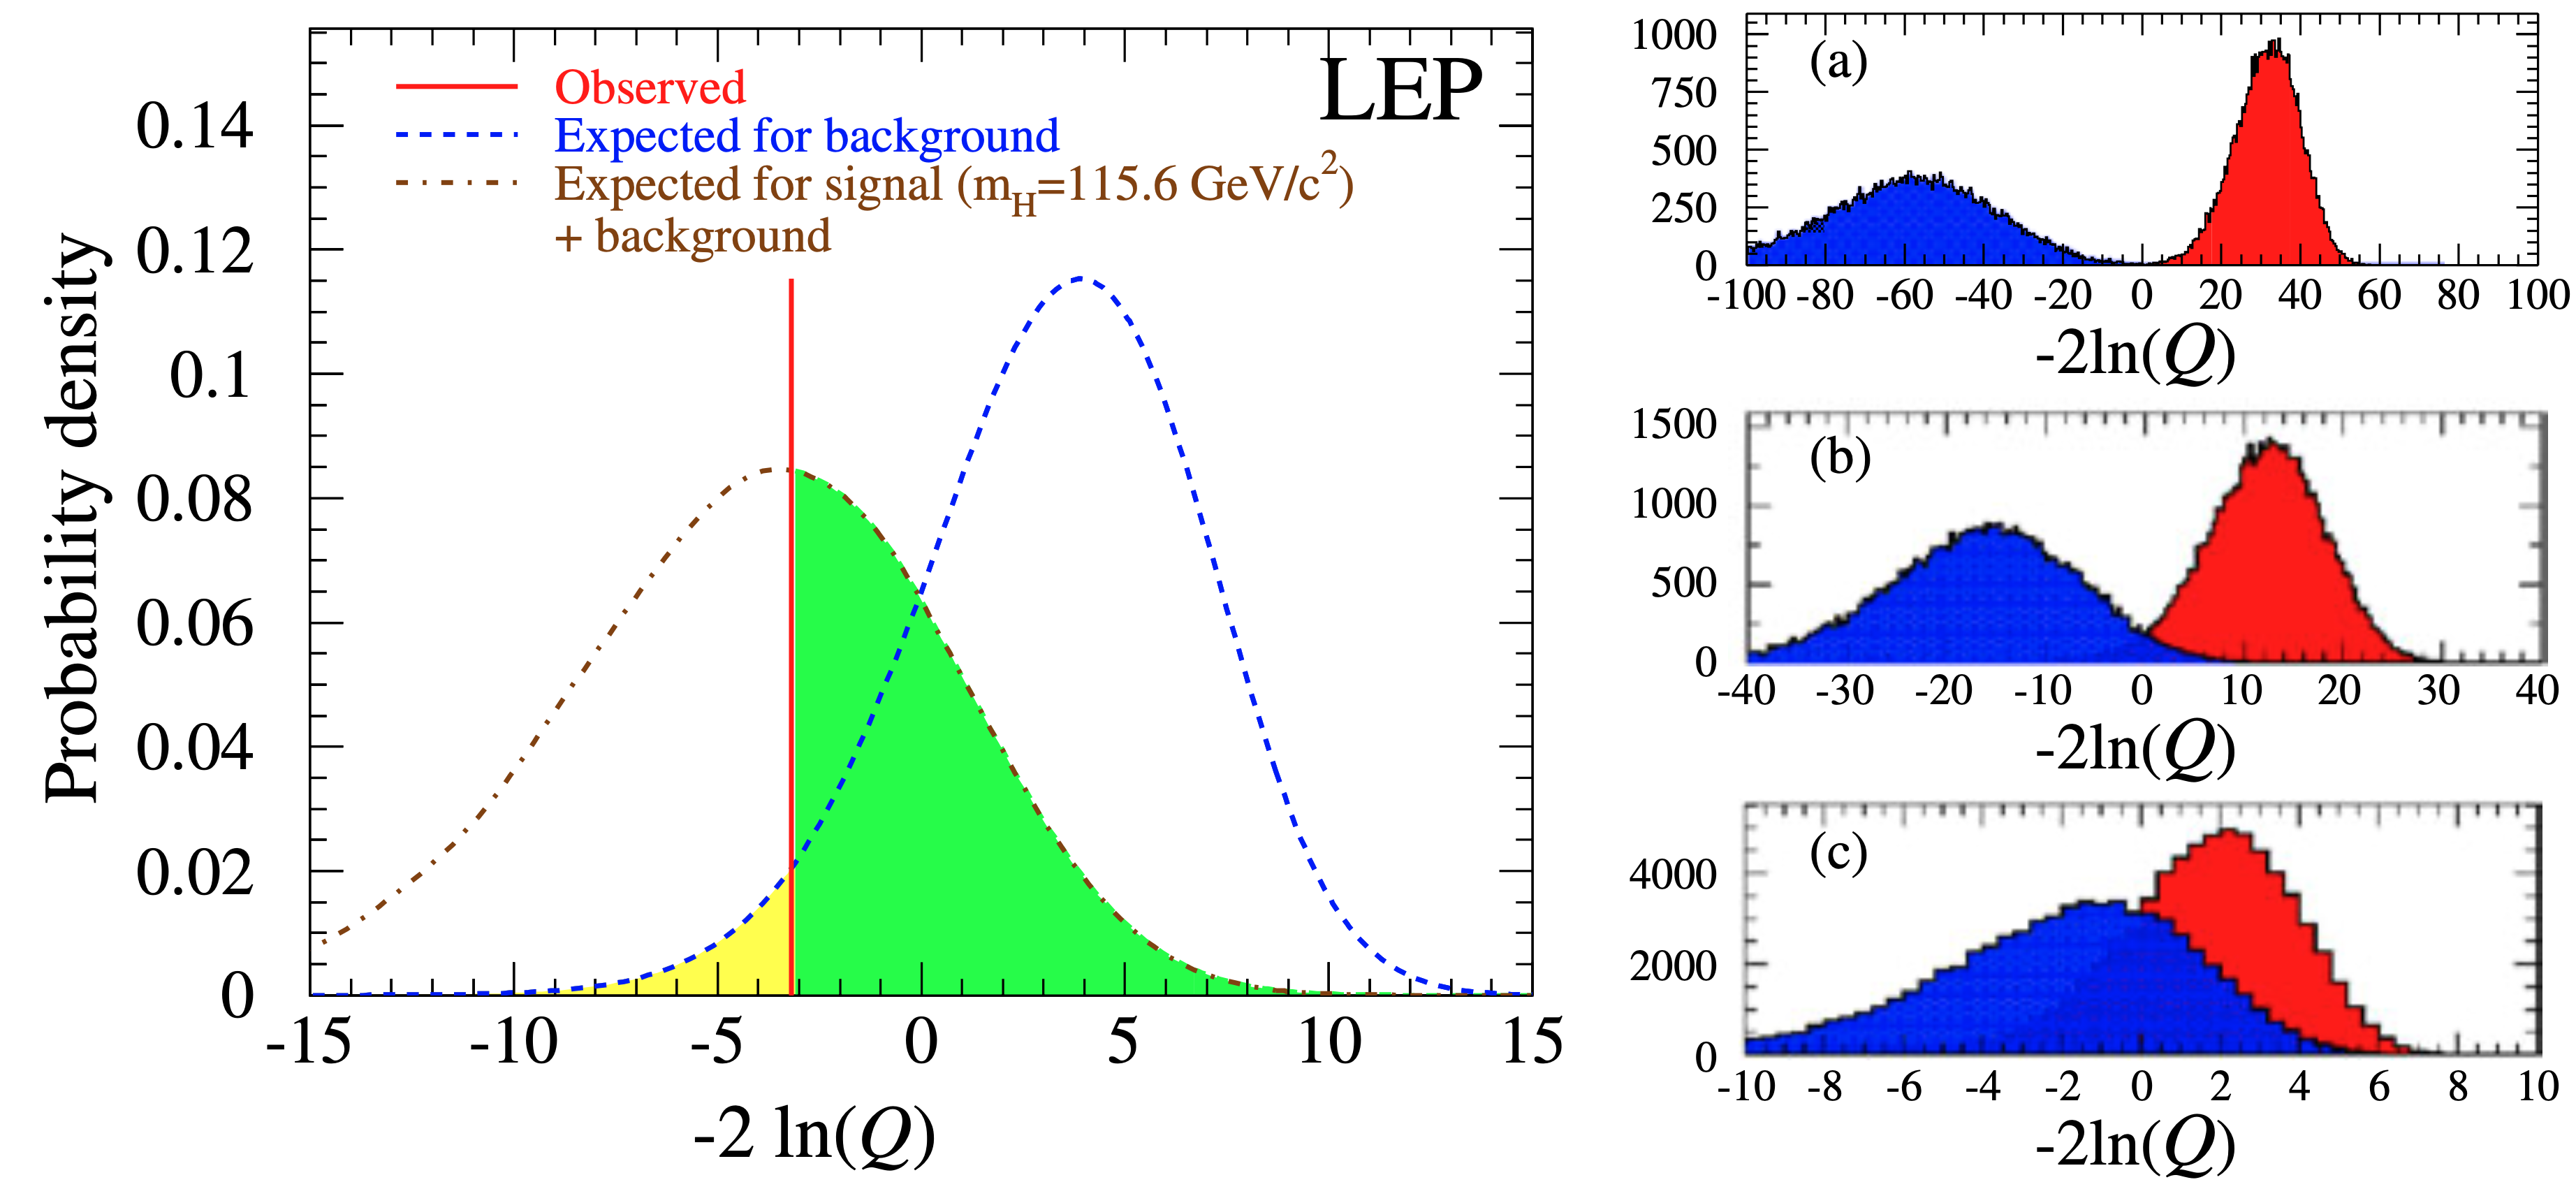
\includegraphics[width=1\textwidth]{cls.png}
        \caption[]{Probability density functions of test statistics from a Higgs search at LEP illustrating the calculation of p-values ($\lambda$ becomes $Q$). (\textbf{left}) The \acp{pdf}'s of the test statistic $f(t_\mu \mid \mu)$ of the signal + background ({\color[HTML]{804000}{$\bm{\diagup}$}}) and background ({\color[HTML]{2100FF}{$\bm{\diagup}$}}) only hypotheses. The p-value is calculated by integration from $t_{\mu,obs}$ (the red observed line ({\color[HTML]{FF0000}{$\bm{\diagup}$}})) to infinity (see eq. \ref{eq:p-value}). The green shaded area (\hexbox{00FF00}) corresponds to $p_{s+b}$ whereas the yellow area (\hexbox{FDFF02}) corresponds to $1-p_b$ since the integral over one whole \acp{pdf} is 1. (\textbf{right}) Degradation of search sensitivity from (a) to (c). Note that the colors of the \acp{pdf}'s change here to signal + background (\hexbox{2100FF}) and background only (\hexbox{FF0000}). For example putting the observation ($t_{\mu,obs}$) on the x-axis at 0 in these plots, one would get for plot (a) $p_{b}\approx 1$ and $p_{s+b}\approx 0$ resulting in a CL$_s\approx 0$, whereas with increasing overlap the CL$_s$ value increases and the sensitivity decreases.
        Taken from \citep{read2002presentation}.}
    \label{fig:cls}    
\end{figure}



\subsection{The HistFactory model}

A model used widely to build a likelihood as described in section \ref{sec:likelihood} is called HistFactory \citep{cranmer2012histfactory} and is implemented within \textsc{pyhf} \citep{pyhf}. This section is based on the introduction to the model within the documentation of \textsc{pyhf}. HistFactory reduces the building of a likelihood into a small number of basic components. For this purpose, it is again useful to think of another splitting of the model parameters $\bm{\phi}$ into

\newcommand{\freeset}{\bm{\eta}}
\newcommand{\constrset}{\bm{\chi}}
\newcommand{\singleconstr}{\chi}
\newcommand{\channelcounts}{\bm{n}}
\newcommand{\auxdata}{\bm{a}}
\newcommand{\poiset}{\bm{\psi}}
\newcommand{\nuisset}{\bm{\theta}}
\newcommand{\fullset}{\bm{\phi}}
\newcommand{\singlefull}{\phi}


\begin{equation}
 L(\bm{x}|\fullset) \quad=\quad
 L(\bm{x}|\overbrace{\poiset}^{\llap{\text{parameters of interest}}},\underbrace{\nuisset}_{\llap{\text{nuisance parameters}}}) \quad=\quad
 L(\bm{x}|\overbrace{\freeset}^{\rlap{\text{free}}},\underbrace{\constrset}_{\rlap{\text{constrained}}}) 
\end{equation}
free parameters $\freeset$ and constrained parameters $\constrset$. Free parameters are free to choose in the model and can be for example a cross-section of a process. Constrained parameters are used to incorporate uncertainties into the likelihood to constrain it. Further there might be several histograms of an observable, for example measured in orthogonal kinematic regions, that are called channels $c$. Bins have the index $b$ here and constraint terms are denoted $c_{\singleconstr}$. With that the likelihood can be described by 
\begin{equation}
L(\channelcounts, \auxdata \,|\,\freeset,\constrset) = \underbrace{\color{blue}{\prod_{c\in\mathrm{\,channels}} \prod_{b \in \mathrm{\,bins}_c}\textrm{Pois}\left(n_{cb} \,\middle|\, \nu_{cb}\left(\freeset,\constrset\right)\right)}}_{\substack{\text{Simultaneous measurement}\\%
\text{of multiple channels}}} \underbrace{\color{red}{\prod_{\singleconstr \in \constrset} c_{\singleconstr}(a_{\singleconstr} |\, \singleconstr)}}_{\substack{\text{constraint terms}\\%
\text{for }\text{auxiliary measurements}}}.
\end{equation}
The $n_{cb}$ is the observation and $\nu_{cb}(\freeset,\constrset)$ the prediction. The $c_{\singleconstr}(a_{\singleconstr} |\, \singleconstr)$ are calculated from auxiliary measurements $a_{\singleconstr}$ (the uncertainties) to constrain the parameter $\singleconstr$ and can be any function (e.g. Gaussian, Poissonian,...) the parameter/uncertainty is believed to be distributed.

The prediction is a sum of nominal bin counts\footnote{also called rates, like in the definition of a Poisson distribution} $\nu_{scb}^0$ over all samples $s$ (e.g. $t\overline{t}$, multijet-background, etc.). These nominal bin counts are subject to uncertainties. Therefore the bin counts can be varied within the bounds of these uncertainties. However the effect of this modification to the likelihood must be taken into account which is through the constraint terms. These penalize the likelihood the larger the modification to a nominal value becomes. The $\nu_{scb}^0$ are varied with multiplicative $\kappa_{scb}$ and additive modifiers $\Delta_{scb}$ 
\begin{align}
    \nu_{cb}\left(\fullset\right) &= \sum_{s\in\mathrm{\,samples}} \nu_{scb}\left(\freeset,\constrset\right)\\ &= \sum_{s\in\mathrm{\,samples}}\underbrace{\left(\prod_{\kappa\in\,\bm{\kappa}} \kappa_{scb}\left(\freeset,\constrset\right)\right)}_{\text{multiplicative modifiers}}\, \Bigg(\nu_{scb}^0\left(\freeset, \constrset\right) + \underbrace{\sum_{\Delta\in\bm{\Delta}} \Delta_{scb}\left(\freeset,\constrset\right)}_{\text{additive modifiers}}\Bigg).
\end{align}
The different types of modifiers are explained in section \ref{sec:modifiers} and the constraint terms $c_{\singleconstr}$ in section \ref{sec:constraint_terms}.

Why this is useful can be seen by considering one uncertainty to a nominal bin count estimate $\nu_{scb}^0$. By modifying $\nu_{scb}^0$ with a factor $\kappa$ in a way that increases the Poisson probability while the corresponding constraint term $c_\kappa(\kappa)$ stays around 1, it can be beneficial for the goal of maximizing the likelihood. This means the most likely/compatible value to the observed data within the modeling of the uncertainties can be found. 

\subsection{The Modifiers}\label{sec:modifiers}
In HistFactory there are by convention four types $\{\lambda,\mu,\gamma,\alpha\}$ of such multiplicative rate modifiers that are explained in this section. There are \textbf{free rate modifiers $\lambda$ and $\mu$} that affect all bins equally, like the cross-section of a process or the luminosity 
\begin{equation}
    \nu_{scb}(\mu)=\mu \nu_{scb}^0.
\end{equation}
These are bin-independent normalization factors and preserve the shape of the histogram. 
Further there are \textbf{bin-wise modifiers} $\gamma_b$ (uncorrelated shape)
\begin{equation}
    \nu_{scb}(\gamma_b)=\gamma_b \nu_{scb}^0.
\end{equation}
These are useful for example to include uncertainties of a per bin data-driven background estimate. This type without a constraint term is not of much use as if there is only one sample or channel, the fit would always match the data perfectly.
In addition there exist \textbf{interpolation parameters $\alpha$} (shape factors) that enter the modeling through an interpolation function $\eta$ instead of being the factor itself. They exist in multiplicative versions 
\begin{equation}
    \nu_{scb}(\alpha)=\eta(\alpha) \nu_{scb}^0,
\end{equation}
and additive versions
\begin{equation}
    \nu_{scb}(\alpha)=\nu_{scb}^0 + \eta(\alpha).
\end{equation}
This is useful to include systematic uncertainties. In a typical ATLAS analysis usually one knows the one standard deviation of a bin count $\eta_{-1}=\nu_{scb}^\mathrm{1down}$ and $\eta_{1}=\nu_{scb}^\mathrm{1up}$ to the nominal value $\nu_{scb}^0$ of an uncertainty. These are used to construct interpolation functions that modify the nominal value with a nuisance parameter that is also used to apply a penalization $c_\alpha$ according to the modeling of the uncertainty.

In HistFactory there exists four of such interpolation functions. For those exist an identity operator 
\begin{equation}
    \eta_0=\eta (\alpha=0) =
    \begin{cases}
        1 ,& \text{multiplicative modifier, } (\kappa) \\
        0 ,& \text{additive modifier, } (\lambda).
    \end{cases}
\end{equation}
One example of these interpolation functions that scales the bin count linearly over the known deviations $\eta_{-1}=\nu_{scb}^\mathrm{1down}$ and $\eta_{1}=\nu_{scb}^\mathrm{1up}$ is
\begin{equation}
    \eta_\mathrm{linear}(\alpha)=
    \begin{cases}
        \alpha(\eta_0 - \eta_1) ,& \alpha>0\\
        \alpha(\eta_0 - \eta_{-1}) ,& \alpha<0
    \end{cases}
\end{equation}
This is illustrated in fig. \ref{fig:interp_func}(a). For the other ones see e.g. \citep{heinrich2019searches}. It is noted that $\alpha$ is the nuisance parameter and not the function $\eta(\alpha)$ and there is an associated constraint term $c_\alpha$ to each $\alpha$.
\begin{figure}
    \centering
    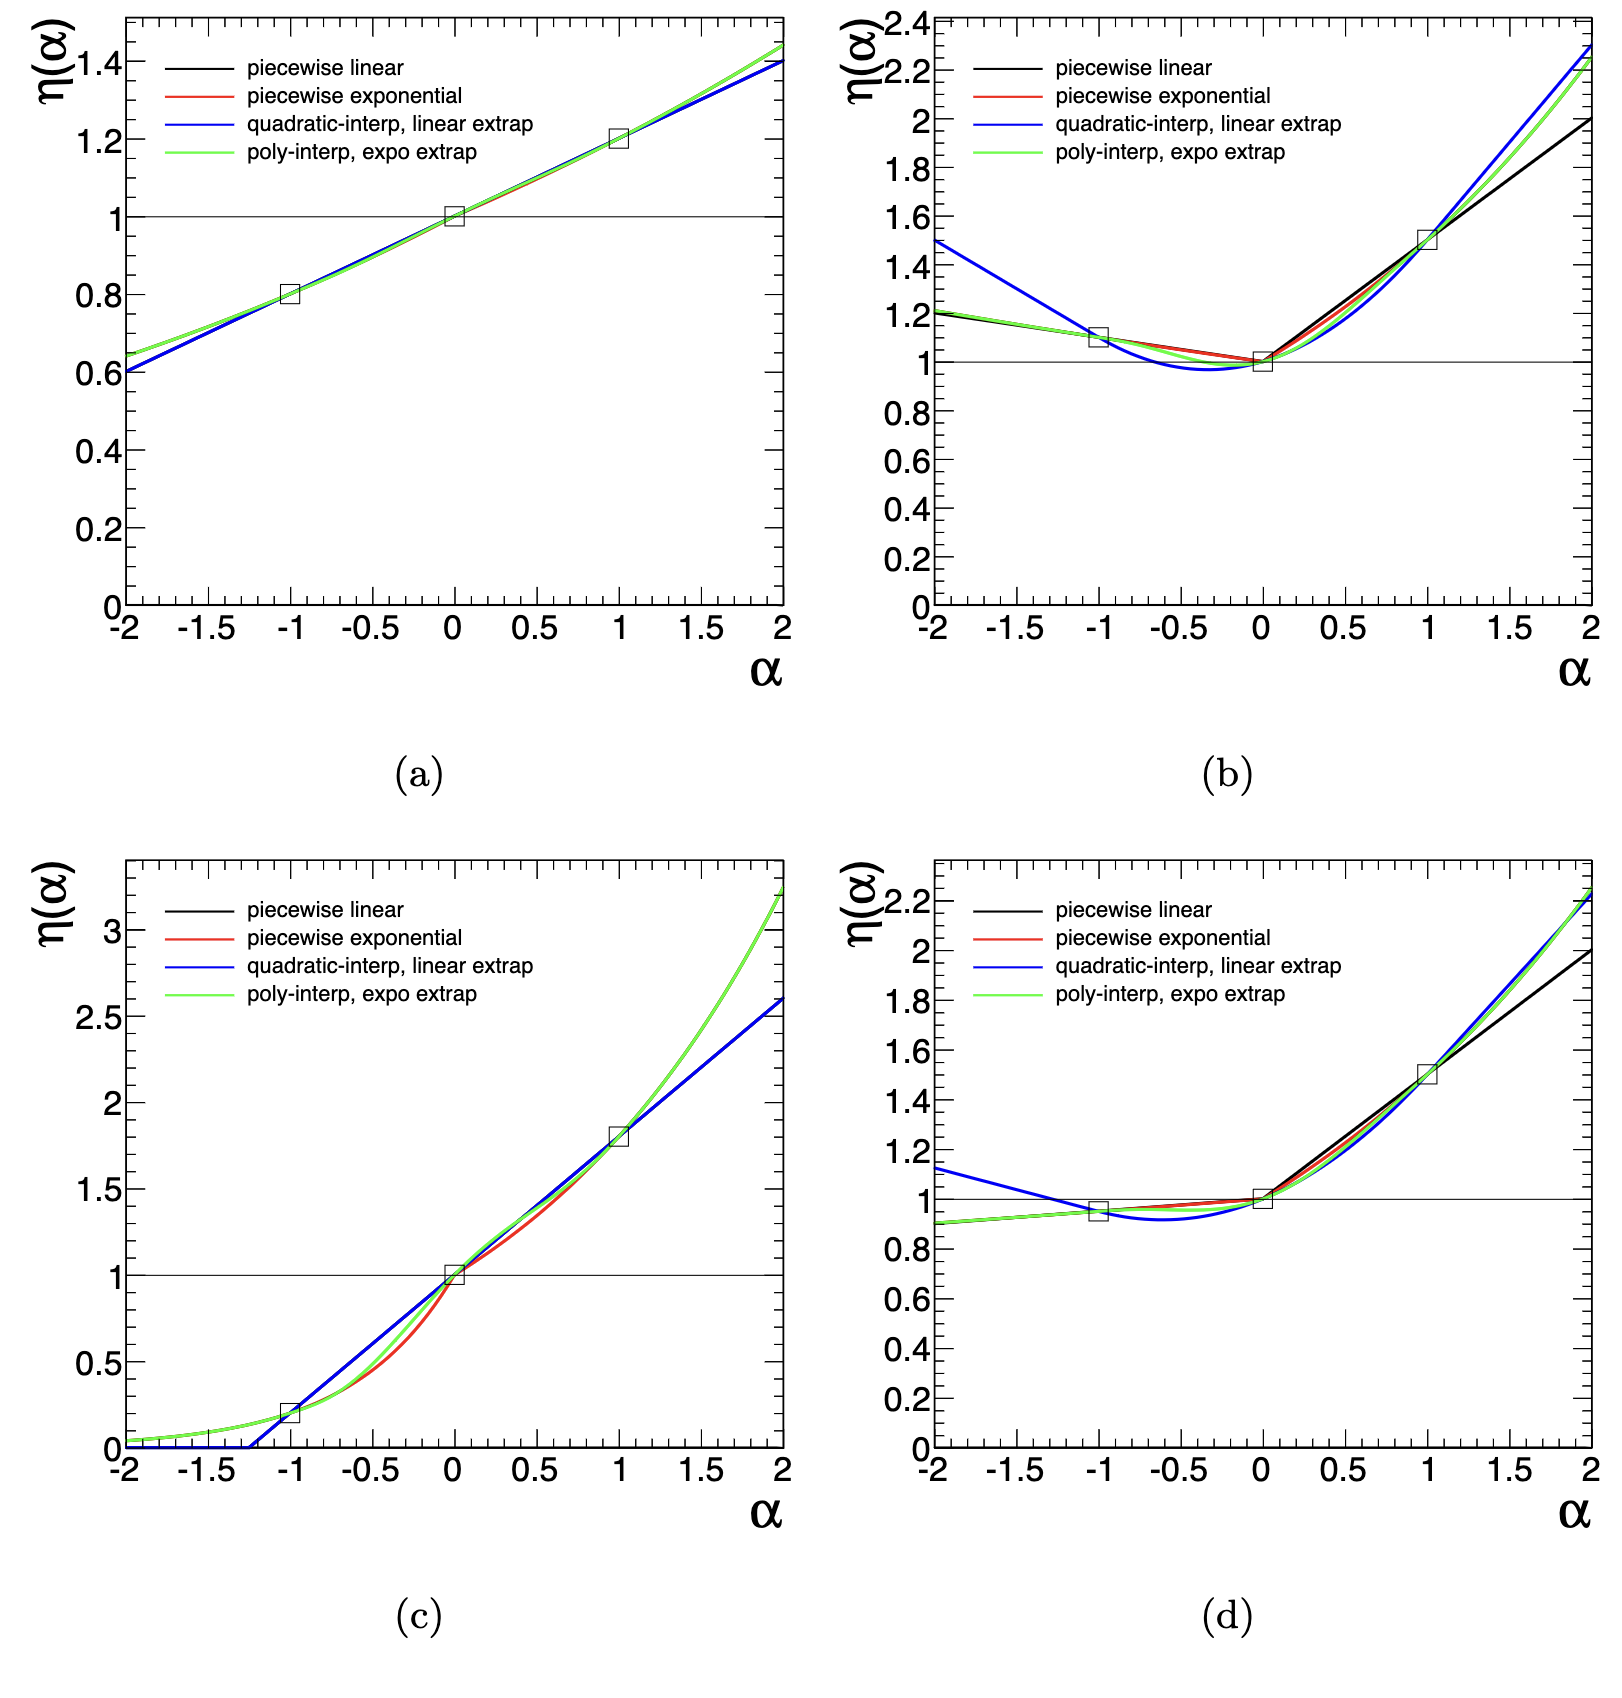
\includegraphics[width=.8\textwidth]{interp_func.png}
        \caption[]{The four interpolation functions $\eta(\alpha)$ for different up and down standard deviation values. For example in (a) the bin count will be scaled with a factor of 0.8 for an $\alpha=-1$ (1.2 for an $\alpha=1$). From \citep{cranmer2012histfactory}.}
    \label{fig:interp_func}    
\end{figure}

\subsection{The constraint terms}\label{sec:constraint_terms}
Uncertainties are modeled either Gaussian or Poissonian. The Gaussian implementation is straightforward as the uncertainty appears squared in the definition. For the interpolation function the nuisance parameter is scaled to the standard deviation values as described before $\mathrm{Gauss}(\alpha \mid a, \sigma=1)$. 

For a Poissonian constraint to a multiplicative modifier $\gamma_b$, with a nominal (most probable) value $\gamma_0=1$, the Poisson distribution must be scaled with a factor $f$, so it reflects the original bin-count uncertainty $\sigma$. To find the corresponding Poisson distribution all parameters are multiplied by a factor $f$ and is then solved for the one with the desired uncertainty. Since the variance of a Poissonian like eq. \ref{eq:poisson} is  the rate parameter $\lambda$ it follows
\begin{equation}
    \mathrm{Var}\left[\mathrm{Pois}(k=f\gamma_0,\lambda=f\gamma)\right]=\lambda\;\stackrel{\gamma=\gamma_0}{=}\;f\gamma_0=(f\sigma)^2  \quad \rightarrow \quad f=(1/\sigma^2).
\end{equation}
This completes all the requirements needed for the creation of HistFactory models. The different types of modifiers and their constraint terms are summarized in table \ref{tab:histfactory}.
\begin{table}[]
    \caption[]{Modifiers and constraint terms used in HistFactory implemented by \textsc{pyhf}. Note that the interpolation functions are called $f_p$ and $g_p$ here instead of $\eta$ as chosen in the full text. Taken from \citep{pyhf}}
    \centering
    \resizebox{0.97\textwidth}{!}{
        \begin{tabular}{l|l|l|l}\label{tab:histfactory}
            Description &Modification&Constraint Term $c_\singleconstr$ &$c_\chi$ input\\
            \hline
            Uncorrelated Shape   &$\kappa_{scb}(\gamma_b) = \gamma_b$                                                                     &$\prod_b \mathrm{Pois}\left(r_b = \sigma_b^{-2}\middle|\,\rho_b = \sigma_b^{-2}\gamma_b\right)$ &$\sigma_{b}$    \\
            Correlated Shape     &$\Delta_{scb}(\alpha) = f_p\left(\alpha\middle|\,\Delta_{scb,\alpha=-1},\Delta_{scb,\alpha = 1}\right)$ &$\displaystyle\mathrm{Gaus}\left(a = 0\middle|\,\alpha,\sigma = 1\right)$                       &$\Delta_{scb,\alpha=\pm1}$    \\
            Normalisation Unc.   &$\kappa_{scb}(\alpha) = g_p\left(\alpha\middle|\,\kappa_{scb,\alpha=-1},\kappa_{scb,\alpha=1}\right)$   &$\displaystyle\mathrm{Gaus}\left(a = 0\middle|\,\alpha,\sigma = 1\right)$                       &$\kappa_{scb,\alpha=\pm1}$    \\
            MC Stat. Uncertainty &$\kappa_{scb}(\gamma_b) = \gamma_b$                                                                     &$\prod_b \mathrm{Gaus}\left(a_{\gamma_b} = 1\middle|\,\gamma_b,\delta_b\right)$                 &$\delta_b^2 = \sum_s\delta^2_{sb}$    \\
            Luminosity           &$\kappa_{scb}(\lambda) = \lambda$                                                                       &$\displaystyle\mathrm{Gaus}\left(l = \lambda_0\middle|\,\lambda,\sigma_\lambda\right)$          &$\lambda_0,\sigma_\lambda$    \\
            Normalisation        &$\kappa_{scb}(\mu_b) = \mu_b$ & & \\
            Data-driven Shape    &$\kappa_{scb}(\gamma_b) = \gamma_b$ & & \\
        \end{tabular}
    }
\end{table}


% \chapter{The ATLAS Experiment at the LHC}

In particle physics scattering blah
In order to probe nature at the smallest scales scattering experiments are conducted as the De Broglie wavelength $\lambda=h/p$ tells that with increasing momentum smaller scales can be explored. At the moment the Large Hadron Colider at CERN (European Organization for Nuclear Research) is not only the largest machine ever built, but also the most powerful particle collider at hand .


The ATLAS detector is situated in a cavern 

\section{The Coordinate System}

\section{The Inner Detector}




\appendix
%*******************************************************
% Acronyms
%*******************************************************

\chapter{Acronyms}
\begin{acronym}[neos]
    \acro{cern}[CERN]{Organisation européenne pour la recherche nucléaire}
    \acro{atlas}[ATLAS]{A Toroidal LHC Apparatus}

    % Theory
    \acro{sm}[SM]{Standard Model}
    \acro{qft}[QFT]{Quantum Field Theory}
    \acro{qcd}[QCD]{Quantum Chromodynamics}
    \acro{qed}[QED]{Quantum Electrodynamics}
    \acro{ew}[EW]{Electroweak}
    \acro{ewsb}[EWSB]{Electroweak Symmetry Breaking}
    \acro{vev}[VEV]{Vacuum Expectation Value}
    \acro{ckm}[CKM]{Cabibbo-Kobayashi-Maskawa}
    \acro{em}[EM]{electromagnetic}
    \acro{ip}[IP]{impact parameter of tracks}
    \acro{ml}[ML]{Machine Learning}
    \acro{neos}[\textsc{neos}]{neural end-to-end-optimized summary statistics}
    \acro{hep}[HEP]{High Energy Physics}



    % Detector
    \acro{lhc}[LHC]{Large Hadron Collider}
    \acro{hllhc}[HL-LHC]{High Luminosity \acs{lhc}}
    \acro{id}[ID]{Inner Detector}
    \acro{sct}[SCT]{semiconductor tracker}
    \acro{trt}[TRT]{transition radiation tracker}
    % \acro{itk}[ITk]{Inner Tracker}
    \acro{ibl}[IBL]{insertable $b$-layer}
    % \acro{em}[EM]{electromagnetic}
    % \acro{lar}[LAr]{liquid argon}
    % \acro{ms}[MS]{muon spectrometer}
    % \acro{rpc}[RPCs]{resistive plate chambers}
    % \acro{tgc}[TGCs]{thin gap chambers}
    % \acro{mdt}[MDTs]{monitored drift tubes}
    % \acrodefplural{mdt}[MDT]{monitored drift tubes}
    % \acro{csc}[CSCs]{cathod strip chambers}
    % \acrodefplural{csc}[CSCs]{Cathod strip chambers}
    \acro{hlt}[HLT]{high level trigger}
    % \acro{roi}[RoI]{region of interest}
    % \acrodefplural{roi}[RoIs]{regions of interest}
    \acro{l1}[L1]{Level-1}
    \acro{pfo}[PFO]{Particle Flow Object}
    \acro{tcc}[TCC]{Track CaloCluster}
    \acro{ufo}[UFO]{Unified Flow Object}
    \acro{jes}[JES]{Jet Energy Scale}
    \acro{jer}[JER]{Jet Energy Resolution}
    \acro{jmr}[JMR]{Jet Mass Resolution}


    % hh4b analysis
    \acro{ggf}[GGF]{gluon-gluon fusion}
    \acro{vbf}[VBF]{vector-boson fusion}
    \acro{nnlo}[NNLO]{next-to-next-to-leading order}
    \acro{nnnlo}[N$^3$LO]{next-to-next-to-next-to-leading order}
    \acro{sr}[SR]{Signal Region}
    \acro{vr}[VR]{Validation Region}
    \acro{cr}[CR]{Control Region}
    \acro{kde}[KDE]{Kernel Density Estimation}
    \acro{bkde}[bKDE]{binned Kernel Density Estimation}

    

    % \acro{pdf}[PDF]{Parton Distribution Function}
    % \acro{dglap}[DGLAP]{Dokshitzer–Gribov–Lipatov–Altarelli–Parisi}
    \acro{mc}[MC]{Monte Carlo}
    % \acro{mpi}[MPI]{multi-parton interaction}
    % \acro{ps}[PS]{parton shower}
    % \acro{me}[ME]{matrix element}
    % \acro{isr}[ISR]{initial state radiation}
    % \acro{fsr}[FSR]{final state radiation}
    % \acro{4fs}[4FS]{four-flavour scheme}
    % \acro{5fs}[5FS]{five-flavour scheme}
    % \acro{nlo}[NLO]{next-to-leading order}
    % \acro{}[]{}

    \acro{pdf}[PDF]{Parton Density Function}


    \acro{pv}[PV]{primary vertex}
    \acro{jvt}[JVT]{jet vertex tagger}

    % \acro{ml}[ML]{Machine Learning}
    % \acro{mle}[MLE]{Maximum Likelihood Estimation}
    % \acro{llr}[LLR]{Log-likelihood ratio}
    % \acro{bdt}[BDT]{Boosted Decision Tree}
    \acro{nn}[NN]{Neural Network}
    \acro{ann}[ANN]{Artificial Neural Network}
    
    % \acro{relu}[\textsc{ReLU}]{Rectified Linear Unit}
    % \acro{adaboost}[AdaBoost]{Adaptive Boost}
    % \acro{HP}{Hyperparameter}


    % btagging
    % \acro{dl1}[DL1]{Deep Learning based heavy-flavour tagger}
    \acro{wp}[WP]{working point}
    \acro{vr}[VR]{variable radius}
    % \acro{ip}[IP]{impact parameter}
    % \acro{sv}[SV]{secondary vertex}
    % \acro{sv1}[SV1]{inclusive displaced secondary vertex reconstruction algorithm}
    % \acro{jf}[JF]{\textsc{JetFitter}}
    % \acro{smt}[SMT]{Soft Muon Tagger}
    % \acro{dips}[DIPS]{Deep Impact Parameter Sets}


    % \acro{sr}[SR]{signal region}
    % \acro{cr}[CR]{control region}
    % \acro{stxs}[STXS]{Simplified Template Cross-Section}

    % \acro{wlcg}[WLCG]{Worldwide LHC Computing Grid}
\end{acronym}

% more package info: https://www.namsu.de/Extra/pakete/Acronym.html
% Befehl	Wirkung
% ac{Kuerzel}	Bei der ersten Verwendung von ac{Kuerzel} wird die Langfassung der Abkürzung und die Abkürzung selbst in Klammern dargestellt. Wird der Befehl ac{Kuerzel} das nächste mal aufgerufen erschneit nur nocht die Abkürzung.
% \acresetall	Der Befehl \acresetall ermöglicht es das Gedächnis des ac Befehls zu löschen. Wird der Befehl \acresetall gesetzt verhält sich der ac Befehl danach wie beim ersten Aufruf (Bei allen bisher gesetzten Abkürzungen).
% acf{Kuerzel}	Mit acf{Kuerzel} gibt es ein zweites Erstes Mal für diese Abkürzung. Das heißt, sie wird wieder in der Langform und der geklammerten Abkürzung gezeigt.
% acs{Kuerzel}	acs{Kuerzel} gibt nur die Abkürzung aus.
% acl{Kuerzel}	acl{Kuerzel} gibt nur die Langform der Abkürzung aus.
% acp{Kuerzel}	Gleiche Wirkung wie ac{Kuerzel} nur hier wird der Plural ausgegeben.
% acfp{Kuerzel}	Gleiche Wirkung wie acf{Kuerzel} nur hier wird der Plural ausgegeben.
% acsp{Kuerzel}	Gleiche Wirkung wie acs{Kuerzel} nur hier wird der Plural ausgegeben.
% aclp{Kuerzel}	Gleiche Wirkung wie acl{Kuerzel} nur hier wird der Plural ausgegeben.
% acfi{Kuerzel}	Die Langform wird kursiv geschrieben, während die Abkürzung mit Kapitälchen dargestellt wird.
% iac{Kuerzel}	Hier wird der Abkürzung (beziehungsweise wenn es das erste Mal ist der Langform mit geklammerter Abkürzung) der unbestimmte englische Artikel a voran gestellt.
% Iac{Kuerzel}	Hier wird der Abkürzung (beziehungsweise wenn es das erste Mal ist der Langform mit geklammerter Abkürzung) der unbestimmte englische Artikel A voran gestellt.
% acused{Kuerzel}	Die Abkürzung wird als gesetzt markiert (gleiche Wirkung wie der ac Befehl) aber nicht angezeigt. Danach zeigt der ac Befehl nur noch die Abkürzung an.
% acsu{Kuerzel}	Zeigt die Abkürzung an und markiert sie als gesetzt.
% aclu{Kuerzel}	Zeigt die Langform an und markiert sie als gesetzt.

%-------------------------------------------------------------

    \thispagestyle{empty}
    \cleardoublepage
    
    \phantomsection
    \bibliography{bib} 
    
\cleardoublepage    
\pagestyle{schluss}
\begin{center}
    \textbf{Statutory Declaration - Eidesstattliche Erklärung}
\end{center}

I declare that I have authored this thesis independently, that I have not used other than the declared sources/ resources and that I have explicitly marked all materials which has been quoted either literally or by content form the used sources.
\par
Hiermit erkläre ich, dass ich die vorliegende Arbeit selbstständig verfasst, andere als die angegebenen Quellen/Hilfsmittel nicht benutzt und die den benutzten Quellen wörtlich und inhaltlich entnommenen Stellen als solche kenntlich gemacht habe.

\begin{flushright}
\vspace{1.5cm}
Berlin, \today
\vspace{2cm}

\makebox[5cm]{\hrulefill}

Frederic Renner
\end{flushright}


\end{document}



